\documentclass[a4paper,10pt]{article}
\usepackage[utf8]{inputenc}

\usepackage[english]{babel}
\usepackage{xcolor}
\usepackage[compact,small]{titlesec}
\usepackage{booktabs}
\usepackage{tabularx}
\usepackage{xltabular}
\usepackage{multirow}
\usepackage{amsfonts,amsmath,amssymb,amsthm}
\usepackage{mathtools}
\usepackage{marginnote}
\usepackage[top=1.8cm, bottom=1.8cm, outer=1.8cm, inner=1.8cm, heightrounded, marginparwidth=2.5cm, marginparsep=0.5cm]{geometry}
\usepackage{enumitem}
\setlist{noitemsep,parsep=2pt}
\newcommand{\highlight}[1]{\textcolor{kuleuven}{#1}}
\usepackage{pythonhighlight}
\usepackage{graphicx}
\usepackage{esdiff}
\usepackage{mathrsfs}
\usepackage{tikz}
\usepackage{tikz-3dplot}
\usepackage{pgfplots}
\usepgfplotslibrary{colormaps}
\usepackage[section]{algorithm}
\usepackage{algorithmic}
%\usepackage{algpseudocode}
\usepackage{listings}
\usepackage{xcolor}

\usepackage{placeins}

\usepackage{caption}
\usepackage{subcaption}
\usepackage[colorinlistoftodos]{todonotes}
\usepackage{verbatim}

\usepackage{siunitx}
\usepackage{multirow}

\usepackage[T1]{fontenc}
\usepackage[utf8]{inputenc}

\usepackage{booktabs}
\usepackage{enumitem}
\usepackage[colorlinks,citecolor=blue,urlcolor=blue,bookmarks=false,hypertexnames=true]{hyperref} 
\usepackage{cite}
\usepackage{cleveref}

\usepackage{lineno}
\usepackage{wrapfig}
\usepackage{booktabs} % Put this in your preamble
% \linenumbers

\lstset{
    language=Matlab,
    basicstyle=\small\ttfamily,
    breaklines=true,
    keywordstyle=\color{blue},
    commentstyle=\color{gray},
    frame=single
}

\allowdisplaybreaks

\DeclareMathOperator*{\argmax}{arg\,max}
\DeclareMathOperator*{\argmin}{arg\,min}


\newtheorem{theorem}{Theorem}[section]
\newtheorem{lemma}[theorem]{Lemma}
\newtheorem{proposition}[theorem]{Proposition}
\newtheorem{corollary}[theorem]{Corollary}
\newtheorem{definition}[theorem]{Definition}
\newtheoremstyle{bluehomework} % name
  {3pt}                        % Space above
  {3pt}                        % Space below
  {}                           % Body font
  {}                           % Indent amount
  {\color{blue}\bfseries}     % Theorem head font
  {.}                          % Punctuation after theorem head
  { }                          % Space after theorem head
  {}                           % Theorem head spec (empty = default)

\theoremstyle{bluehomework}
\newtheorem{homework}{Question}

\numberwithin{equation}{section}
\crefname{subsection}{subsection}{subsections}
\crefname{equation}{}{}

\title{Inverted Pendulum} 
\author{Arno Genicot \& Stefan Markovsky}
%\date{\today}

\newcommand{\ReplaceMe}[1]{{\color{blue}#1}}
\newcommand{\RemoveMe}[1]{{\color{purple}#1}}
\newcommand{\red}[1]{\textcolor{red}{#1}}
\newcommand{\green}[1]{\textcolor{green}{#1}}

\begin{document}
\fontfamily{ppl}
\selectfont{}

\maketitle

\section{Model and Open Loop Analysis}

\subsection{Linear State Space Representation}

For the inverted pendulum system, the linear state equation $\dot{\mathbf{x}} = A\mathbf{x} + B\mathbf{u}$ becomes 

\begin{equation} \label{eq:state_eq}
  \begin{bmatrix} 
    \dot{x} \\
    \dot{\alpha} \\
    \ddot{x} \\
    \ddot{\alpha} \\  
  \end{bmatrix}
  = 
  \begin{bmatrix} 
    0 && 0 && 1 && 0 \\
    0 && 0 && 0 && 1 \\
    0 && -4.5277 && -16.8835 && 0 \\
    0 && 47.0088 && 55.3557 && 0 \\
  \end{bmatrix}
  \begin{bmatrix} 
    x \\
    \alpha \\
    \dot{x} \\
    \dot{\alpha} \\  
  \end{bmatrix} 
  + 
  \begin{bmatrix}
    0 \\
    0 \\
    3.7778 \\
    -12.3862 \\
  \end{bmatrix}V.
\end{equation}
The state variables are 

\begin{itemize}
  \item $x$: \textbf{The position of the cart}, measured in meters. The position of the cart is measured corresponding to some reference point that indicates the zero position. This point is taken approximately at the middle of the track.
  \item $\alpha$: \textbf{The angular position of the rod} in radians. The angle zero radians correspond to a rod that is upright. A positive angle will correspond to a rod that leans to the right and conversely. 
  \item $\dot{x}$: \textbf{The velocity of the cart}, measured in meters per second.
  \item $\dot{\alpha}$: \textbf{The velocity of the angular position of the rod}, measured in radians per second.
\end{itemize}
A general state-space representation has the form:

\begin{equation} \label{eq:general_ss}
  \begin{cases}
    \dot{\mathbf{x}} &= A\mathbf{x} + B\mathbf{u} \\
    \mathbf{y} &= C\mathbf{x} + D\mathbf{u}. \\
  \end{cases}
\end{equation}
Ultimately, the goal of this project is to design a working state-feedback controller for a real-life setup. Consequently, to compute the control action, $\mathbf{u}=-K\mathbf{x}$, the input to the control module must provide the states $\mathbf{x}$. Since \textbf{the input, $\mathbf{u}$, has no instantaneous influence on the ouput, $\mathbf{y}$, $D = \mathbf{0}$}.\\
\\
In section \ref{closed_loop}, a first closed-loop system is designed. To easily analyze the controller, we assume an ideal environment. All states from equation (\ref{eq:state_eq}) are available with no additional noise. This corresponds to \textbf{$C$ equal to the identity matrix}. Of course, these assumptions are not realistic and do not coincide with the sensors that are used in the real-life setup.\\
\\
In section \ref{realistic_closed_loop}, a more realistic closed loop system is designed. The aim is to simulate the real-life setup more accurately. Because the setup only consists of sensors that measure the position of the cart, $x$, and the angle of the rod, $\alpha$, $C$ must be appropriately chosen, such that $\mathbf{y}$ consists of the measurable states. Consequently, 

\begin{equation}
  C = 
  \begin{bmatrix}
    1 && 0 && 0 && 0 \\
    0 && 1 && 0 && 0
  \end{bmatrix}.
\end{equation}
\textbf{This $C$ is used in the open loop analysis}.

\subsection{Open Loop Analysis}

We can determine the stability of the system by analyzing the eigenvalues of $A$. 

\begin{equation}
  \text{eig}(A) = 
  \begin{bmatrix}
    0 \\
    6.0048787 \\
    -5.0773709 \\
    -17.8109883 \\
  \end{bmatrix}
\end{equation}
\textbf{The system is unstable} (as expected), since it consists of an eigenvalue in the right-half plane. The system does not consist of transmission zeros. \textbf{The system is controllable} since the rank of the controllability matrix, $\mathcal{C}(A,B)$, is four. THis will allow us to place the poles of the closed loop system wherever we want. \textbf{The system is observable}, since the rank of the observability matrix, $\mathcal{O}(A, C)$, is four. Consequently, the observability and the controllability properties imply that \textbf{the system is minimal}. This implies further that the poles are equal to the eigenvalues of $A$. Since the system is controllable, all unstable modes are also controllable and \textbf{the system is stabilizable}. Since the system is observable, all unstable modes are observable and \textbf{the system is detectable}.

\subsection{Control Goals}

The primary objective of the controller is to \textbf{stabilize the inverted pendulum system} by keeping the rod in the upright equilibrium position through manipulation of the DC motor voltage. In addition, the controller must be capable of \textbf{tracking a desired cart position setpoint} in real time while maintaining closed-loop stability. \\
\\
The closed-loop response should exhibit a \textbf{fast settling time} with \textbf{limited overshoot} and \textbf{smooth cart motion}. Furthermore, the \textbf{control action} should remain \textbf{within the physical limitations of the actuator} in order to avoid voltage saturation. Finally, the controller should be sufficiently \textbf{robust against external disturbances} and small modeling inaccuracies, such that the pendulum can recover from perturbations while preserving stable operation.



\section{LQR Controller and a First Closed Loop Model} \label{closed_loop}

In this section, we assume that the entire state vector is available and therefore the matrix $C$ is set to the identity matrix. 

\subsection{Simulink Diagram}

\begin{figure}[htbp]
    \centering
    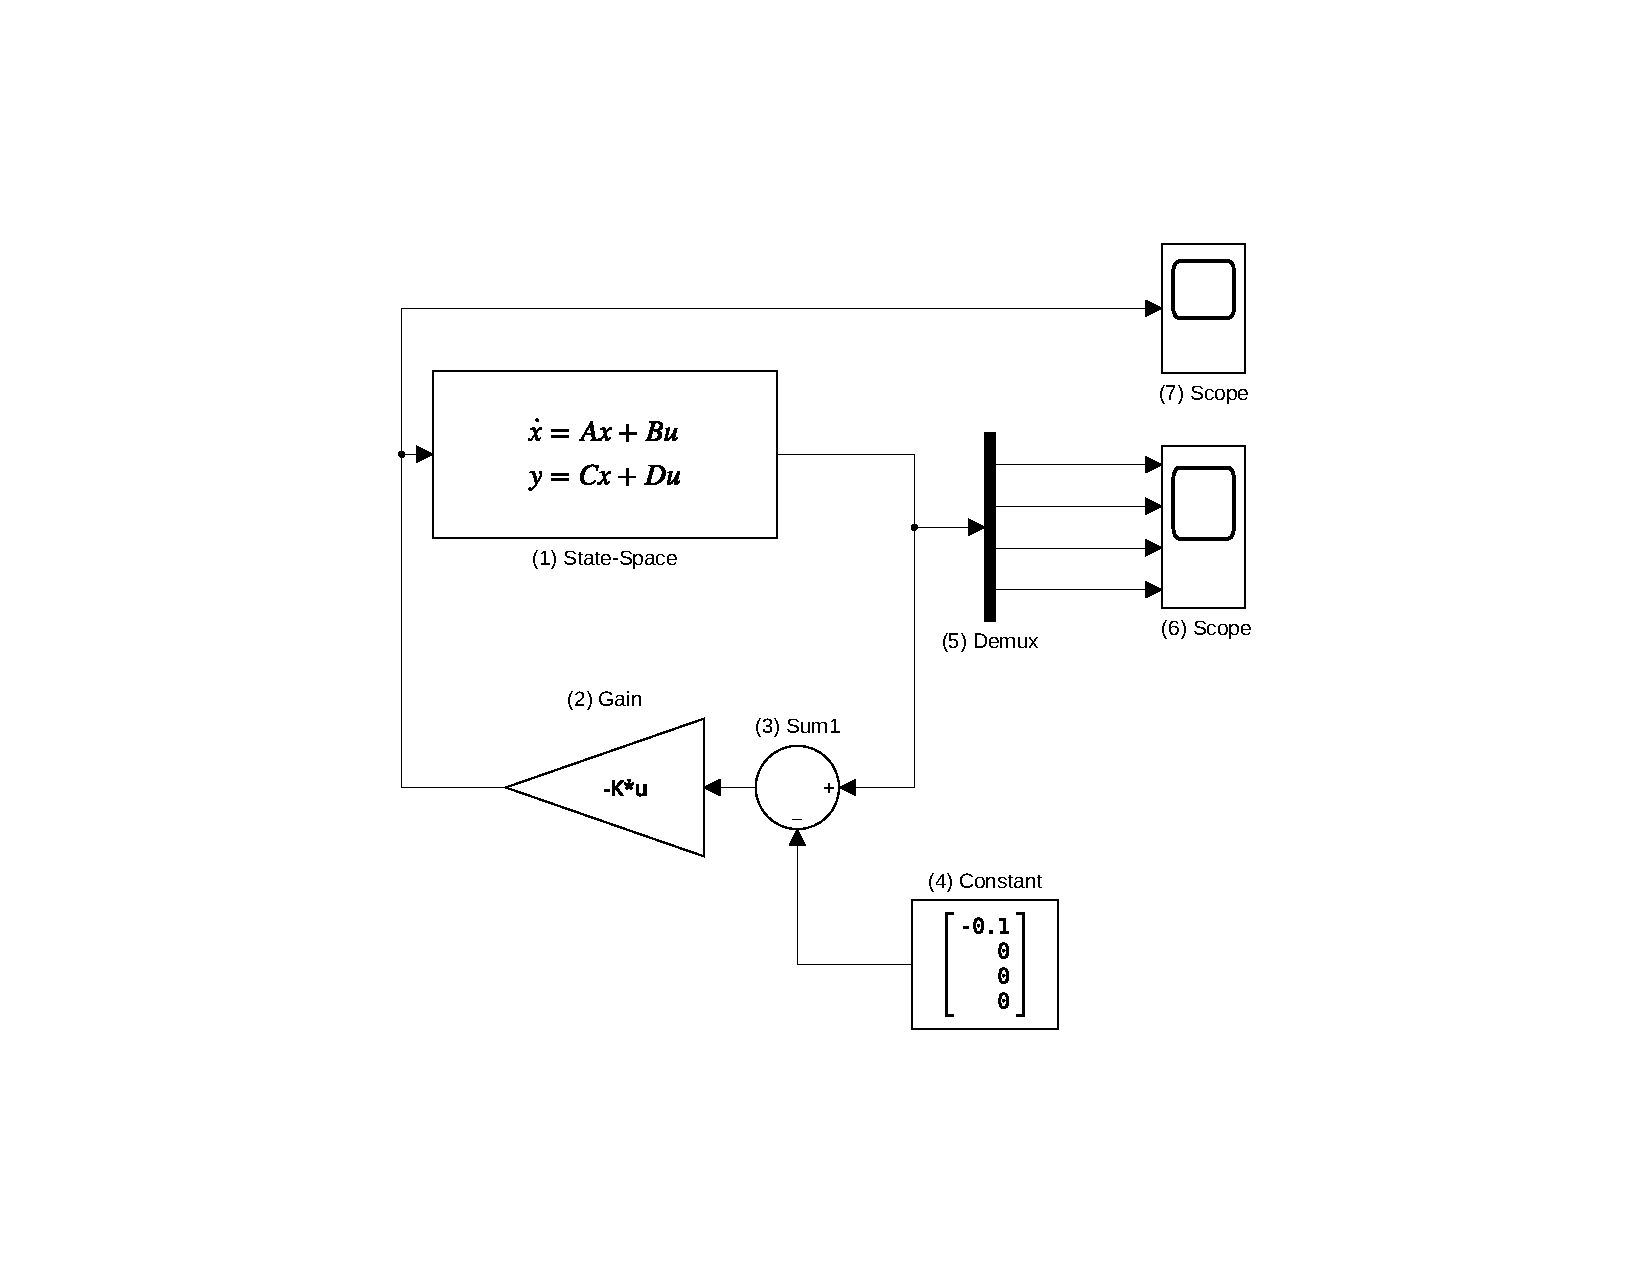
\includegraphics[width=0.8\textwidth]{figures/closed_loop.pdf}
    \caption{Closed loop simulink diagram.}
    \label{fig:closed_loop}
\end{figure}

Figure \ref{fig:closed_loop} provides the simulink diagram of the closed loop system. The diagram contains the following blocks

\begin{itemize}
  \item \textbf{(1) State-Space}: contains the state-space representation, equation (\ref{eq:general_ss}), of the inverted pendulum system. This block applies the input $\mathbf{u}$, which is provided by the ingoing arrow, to the system and outputs $\mathbf{y}$ through the outgoing arrow. The block is initialised with an initial state, $\mathbf{x_0 = 0}$, and the state, $\mathbf{x}$, is updated for each incoming input.     
  \item \textbf{(2) Gain}: realises the control-law. The input is $\mathbf{x - x_{\text{des}}}$ and the ouput is control action, $\mathbf{u} = -K(\mathbf{x-x_{\text{des}}}$). The control action is directly fed to the (1) State-Space block.
  \item \textbf{(3) Sum1}: applies the desired set point to the state of the system, $\mathbf{x-x_{\text{des}}}$. A linear stable system will bring the states to zero. By subtracting the desired cart position from the actual state, the system will bring the new state to zero by moving the cart to the desired position.  
  \item \textbf{(4) Constant}: holds the desired set point of the cart position in a four dimensional vector. 
  \item \textbf{(5) Demux}: deconstructs the four dimensional state vector from (1) State-Space, $\mathbf{x}$, into 4 separate signals. 
  \item \textbf{(6) Scope}: plots the output states of (1) State-Space in time. 
  \item \textbf{(7) Scope}: plots the control input in time.
\end{itemize}

\subsection{Tuning Experiments of the LQR Controller}

In this section, we are interested in finding a good pair, $Q$ and $R$, to compute a controller $K$ that satisfies the control goals previously described. We will perform experiments by varying the diagonal elements of $Q$ and $R$ while keeping all other elements equal to the base values given in the assignment.

\begin{equation}
  Q_{\text{base}} = 
  \begin{bmatrix}
     0.25 && 0 && 0 && 0 \\
    0 && 4 && 0 && 0 \\
    0 && 0 && 0 && 0 \\
    0 && 0 && 0 && 0 \\
  \end{bmatrix}, \quad
  R_{\text{base}} = 0.003.
\end{equation}
For each experiment, we will plot the states, the control action, and the poles of the closed loop system. The poles of the closed loop system are the eigenvalues of $A-BK$. Since the system is minimal, the poles of the closed loop system are also the eigenvalues of $A-BK$. The poles of the closed loop system determine the stability and the transient response of the system. For a stable system, all poles must be in the left half-plane. The further left the poles are, the faster the transient response will be. However, if the poles are too far left, this may lead to a large control action that may exceed the physical limitations of the actuator. Therefore, we want to find a good balance between a fast transient response and a control action that remains within the physical limitations of the actuator.\\
\\
The goal of the experiments is to build understanding on how each element of $Q$ and $R$ affects the system. This understanding will allow us to find a good pair, $Q$ and $R$, that satisfies the control goals. We will write down our observations and  discuss the trade-offs that are made when varying each element of $Q$ and $R$. We are also interested in the effective range of each element. This will provide intuition on how much we can vary each element without drastically affecting the system. We want to avoid blindly adjusting the elements of $Q$ and $R$ without understanding the effects of these adjustments. 

\subsubsection{$Q_{1,1}$}

Figure \ref{fig:q11} plots the results of varying $Q_{1,1} \in \{0.1, 0.25, 0.5, 1.0, 2.0, 5.0, 10.0, 20.0\}$. Increasing $Q_{1,1}$ leads to a faster settling time. However, this also leads to a larger control action that may exceed the physical limitations of the actuator. If the actuator saturates, the system is essentially operating in open-loop since the control action is not present. The system is therefore unstable. It is crucial to avoid continuous periods of saturation, since the system is then unstable in these periods. We also notice that for $Q_{1,1} = 20.0$, the control action exceeds the physical limitations of the actuator and the peaks of the other three states are much bigger. The combination of these two effects may lead to a failure in the real-life setup. As $Q_{1,1}$ increases, the poles of the closed loop system move further left, which corresponds to a faster transient response.\\
\\
We can conclude that increasing $Q_{1,1}$ may improve the settling time of the cart, but can have drastic effects on the control action and all other states. Increasing $Q_{1,1}$ must be done with caution, but if a fast response time of the cart is the primary concern, then a higher value of $Q_{1,1}$ might be acceptable. If the cart is too slow, then increasing $Q_{1,1}$ is a good option to speed up the system.


\subsubsection{$Q_{2,2}$}

Figure \ref{fig:q22} plots the results of varying $Q_{2,2} \in \{1.0, 4.0, 8.0, 16.0, 32.0\}$. Increasing $Q_{2,2}$ leads to a faster settling time and a smaller overshoot of the angle of the rod. The same could be said for the states $\dot{x}$ and $\dot{\alpha}$. However, $x$ is negatively affected. By increasing $Q_{2,2}$, the settling time is reduced for $x$. The peaks of the control action decreases as $Q_{2,2}$ increases. When increasing $Q_{2,2}$, the voltage at $t = 0$ does not change, whereas for $Q_{1,1}$ the voltage becomes larger in magnitude at $t = 0$.\\
\\
In general, increasing $Q_{2,2}$ has a stabilizing effect on the system. The peak of the control action becomes smaller and the states $\alpha, \dot{\alpha}, \dot{x}$ are less volatile. However, the downside is that the settling time of $x$ is increased. Whenever the controller is too aggressive, it is a good idea to increase $Q_{2,2}$ to stabilize the system and reduce the control action. If we compare how fast the settling time of $x$ decreases as $Q_{2,2}$ increases with $Q_{1,1}$ decreases, we can see that reducing the settling time of $x$ by increasing $Q_{1,1}$ is more effective than reducing the settling time of $x$ by increasing $Q_{2,2}$. Therefore, if we want to speed up the system, it is better to increase $Q_{1,1}$ than to increase $Q_{2,2}$. Conversely, if we are happy with a certain settling time of $x$ and we want to reduce the control action and in slow down the other states, it is better to increase $Q_{2,2}$ than to decrease $Q_{1,1}$.

\subsubsection{$Q_{3,3}$ and $Q_{4,4}$}

Figure \ref{fig:q33} plots the results of varying $Q_{3,3} \in \{0.0, 0.1, 0.5, 1.0, 2.0, 5.0, 10.0\}$ and figure \ref{fig:q44} plots the results of varying $Q_{4,4} \in \{0.0, 0.1, 0.5, 1.0, 2.0, 5.0, 10.0\}$. The effects of varying $Q_{3,3}$ and $Q_{4,4}$ are similar as with $Q_{2,2}$. We notice from the figures, that increasing $Q_{3,3}$ and $Q_{4,4}$ reduces the overshoots of the states $\alpha, \dot{\alpha}$ and $\dot{x}$. The main effect of $Q_{3,3}$ is to supress the settling time of $\dot{x}$ and of $Q_{4,4}$ is to supress the settling time of $\dot{\alpha}$. This is observed in the figures. The control action reacts in the same way as in the experiment with $Q_{2,2}$. The voltage at $t = 0$ does not change when increasing $Q_{3,3}$ and $Q_{4,4}$, although the peaks do become smaller. The settling time of $x$ increases as $Q_{3,3}$ and $Q_{4,4}$ increases.\\
\\
The main difference between $Q_{2,2}$ with $Q_{3,3}$ and $Q_{4,4}$ can be seen in the evolution of the poles. We notice that increasing $Q_{2,2}$ moves the poles to the left. Whereas, increasing $Q_{3,3}$ or $Q_{4,4}$ moves the poles mainly towards the real axis. This means that increasing $Q_{3,3}$ and $Q_{4,4}$ has a bigger effect on the oscillatory behavior of the system than increasing $Q_{2,2}$. For now this is not a concern since the system has no noise present. The evolution is theoretically evolving smoothly towards the equilibrium point. However, in the real-life setup, there will be noise present and the system will not evolve smoothly towards the equilibrium point. The system will be perturbed by the noise and the steady state error will not be zero anymore. In this case, it is important to have a good damping of the system to reduce the oscillations around the equilibrium point. Therefore, increasing $Q_{3,3}$ and $Q_{4,4}$ might be a good idea to improve the damping of the system and reduce the oscillations around the equilibrium point. \\
\\
The difference between $Q_{3,3}$ and $Q_{4,4}$ is that increasing $Q_{3,3}$ has a bigger effect on the state $\dot{x}$, whereas increasing $Q_{4,4}$ has a bigger effect on the state $\dot{\alpha}$. We also observe that $Q_{3,3}$ is more sensitive to changes in the system than $Q_{4,4}$. This can be seen in the difference of the change of the state $x$ when increasing $Q_{3,3}$ versus $Q_{4,4}$. The settling time of $x$ when $Q_{3,3} = 10$ is much longer than when $Q_{4,4} = 10$. This observation also applies to the control action. So, increasing $Q_{3,3}$ must be done with caution as it can have great negative impact on the settling time of $x$, whilest varying $Q_{4,4}$ is more ideal for fine-tuning a desired behaviour.\\

\subsubsection{$R$}

Figure \ref{fig:r} plots the results of varying $R \in \{0.001, 0.003, 0.005, 0.01, 0.03, 0.05\}$. Increasing $R$ leads to a smaller control action. Although, the experiments for $Q_{2,2}, Q_{3,3}$ and $Q_{4,4}$ also exhibit this property, $R$ can reduce the Voltage at $t = 0$. Of course the downside is that the system becomes less responsive. The settling time of $x$ can be seen to increase as $R$ increases and the overshoot of the remaining states diminishes. From the plot of the poles, we notice that the main effect of $R$ is to move the non-dominant poles towards the origin.\\

\begin{figure}[htbp]
  \centering
  \begin{subfigure}{0.45\textwidth}
    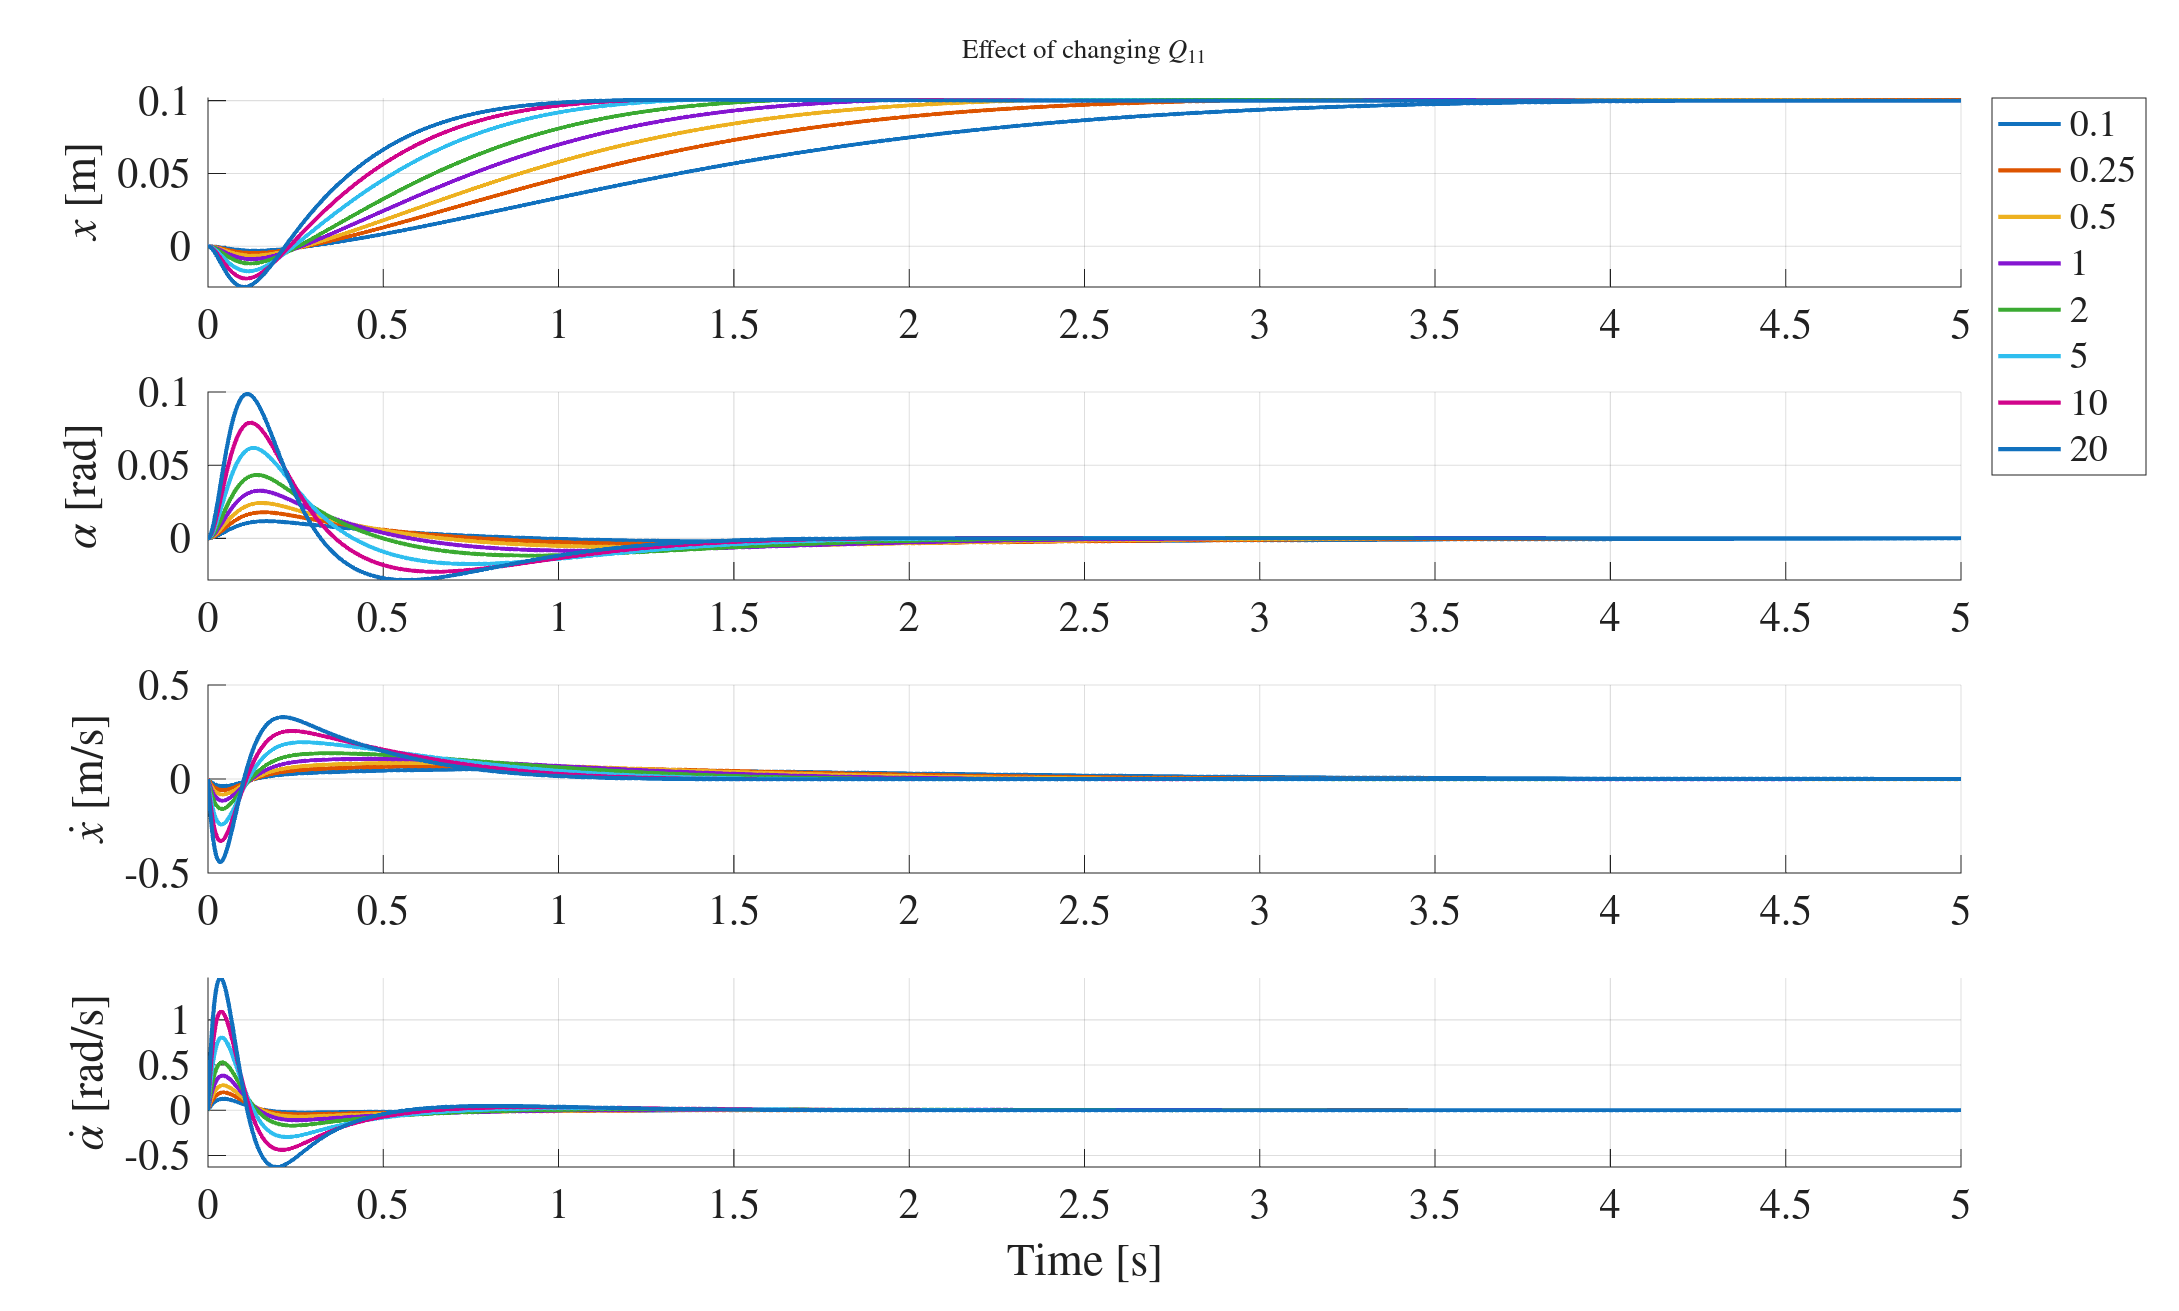
\includegraphics[width=\linewidth]{figures/q11_states.png}
    \caption{States evolution.}
  \end{subfigure}
  \begin{subfigure}{0.45\textwidth}
    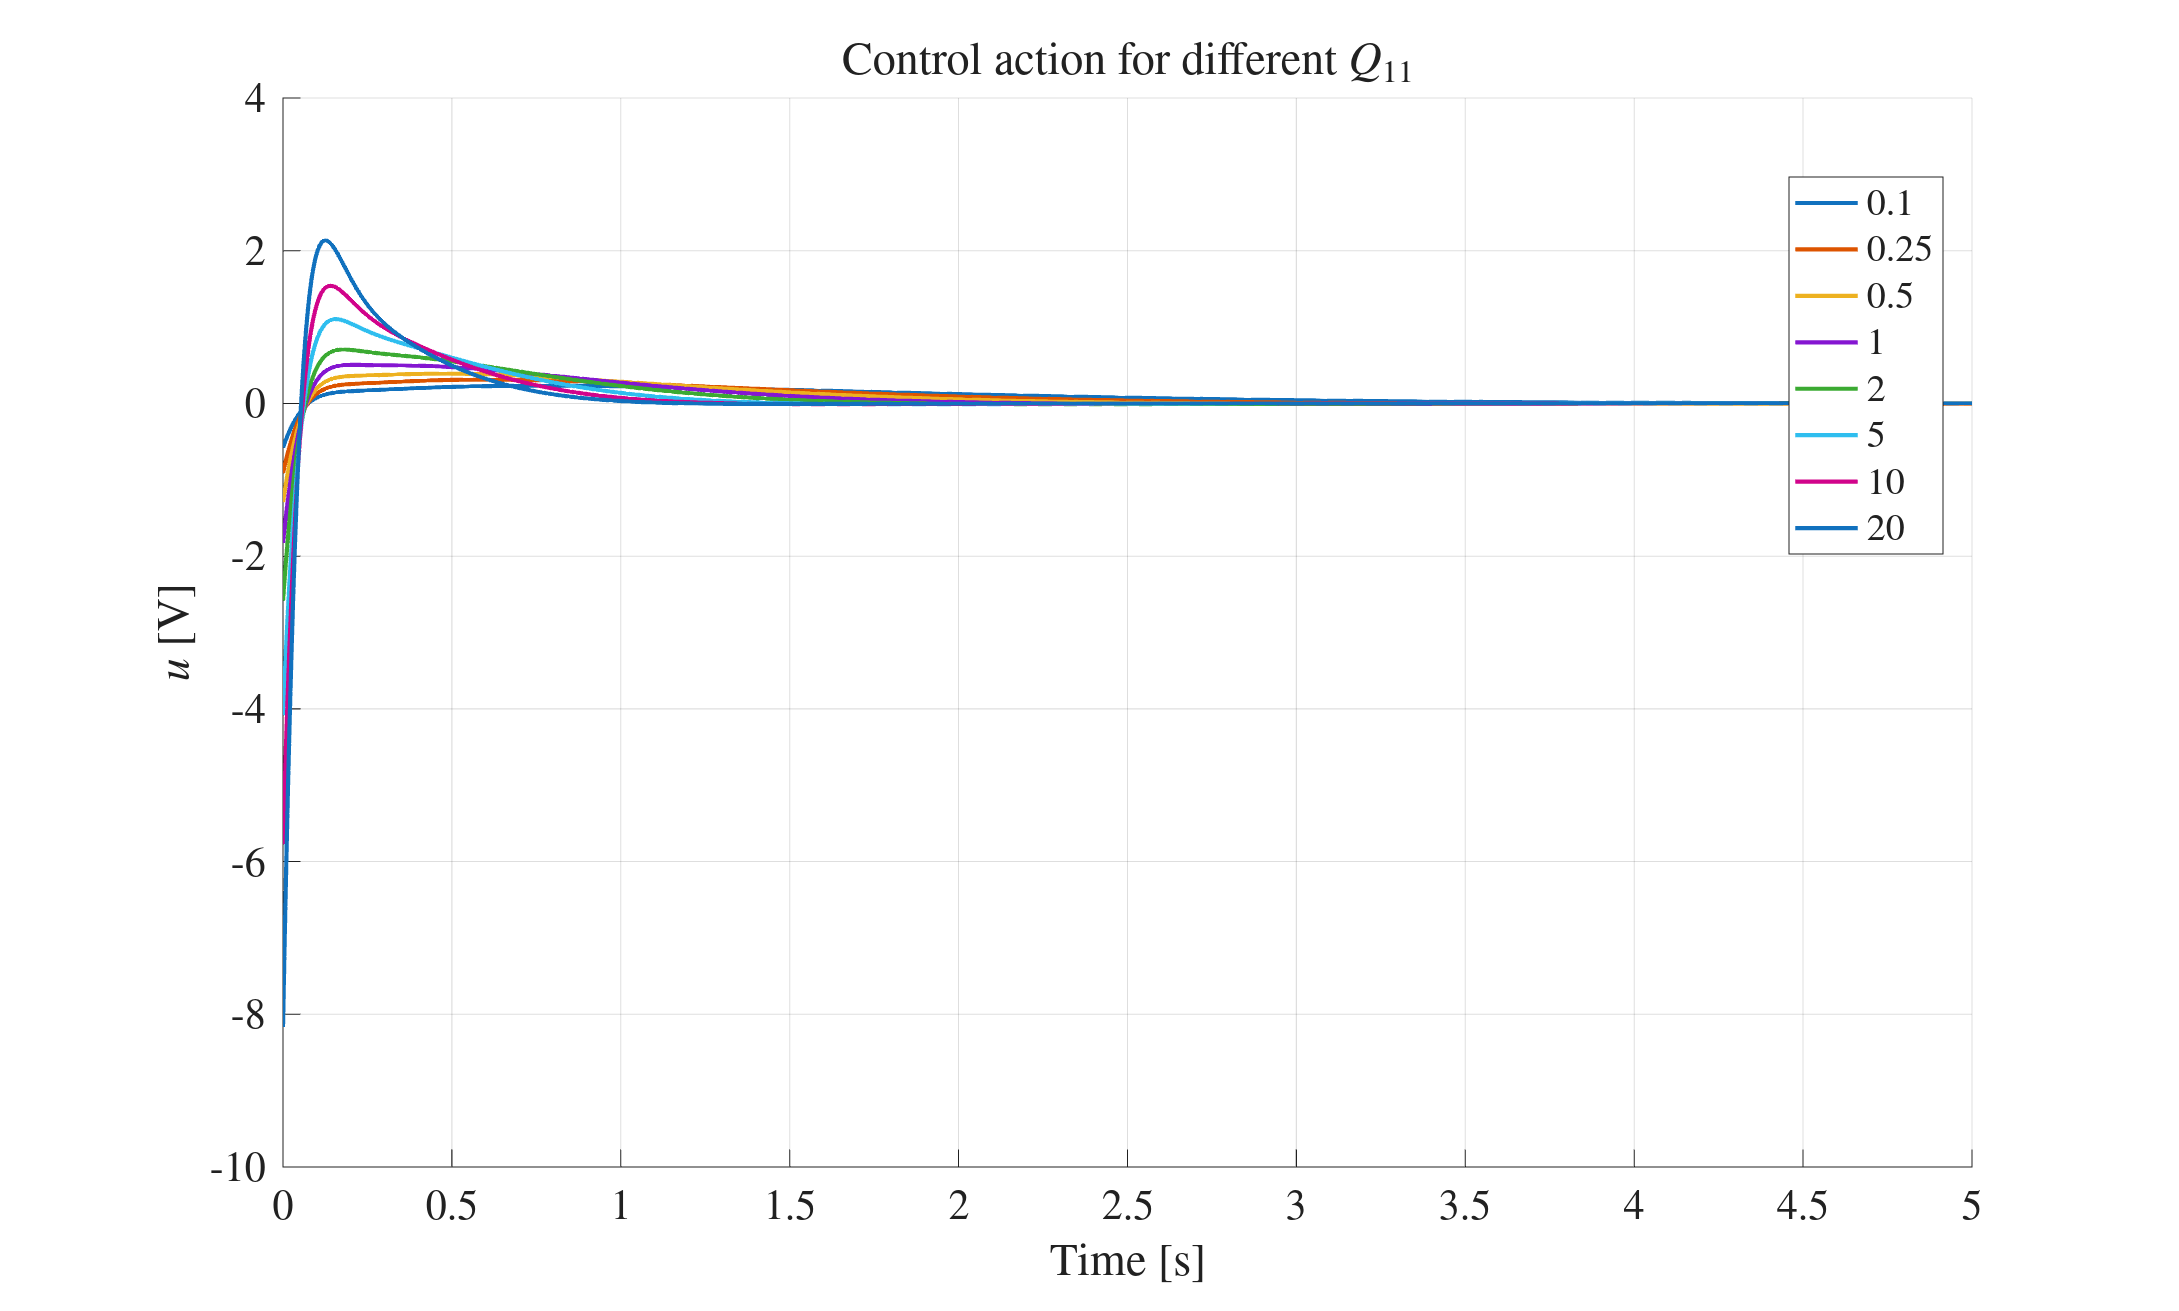
\includegraphics[width=\linewidth]{figures/q11_voltage.png}
    \caption{Control action evolution.}
  \end{subfigure}
  \begin{subfigure}{0.45\textwidth}
    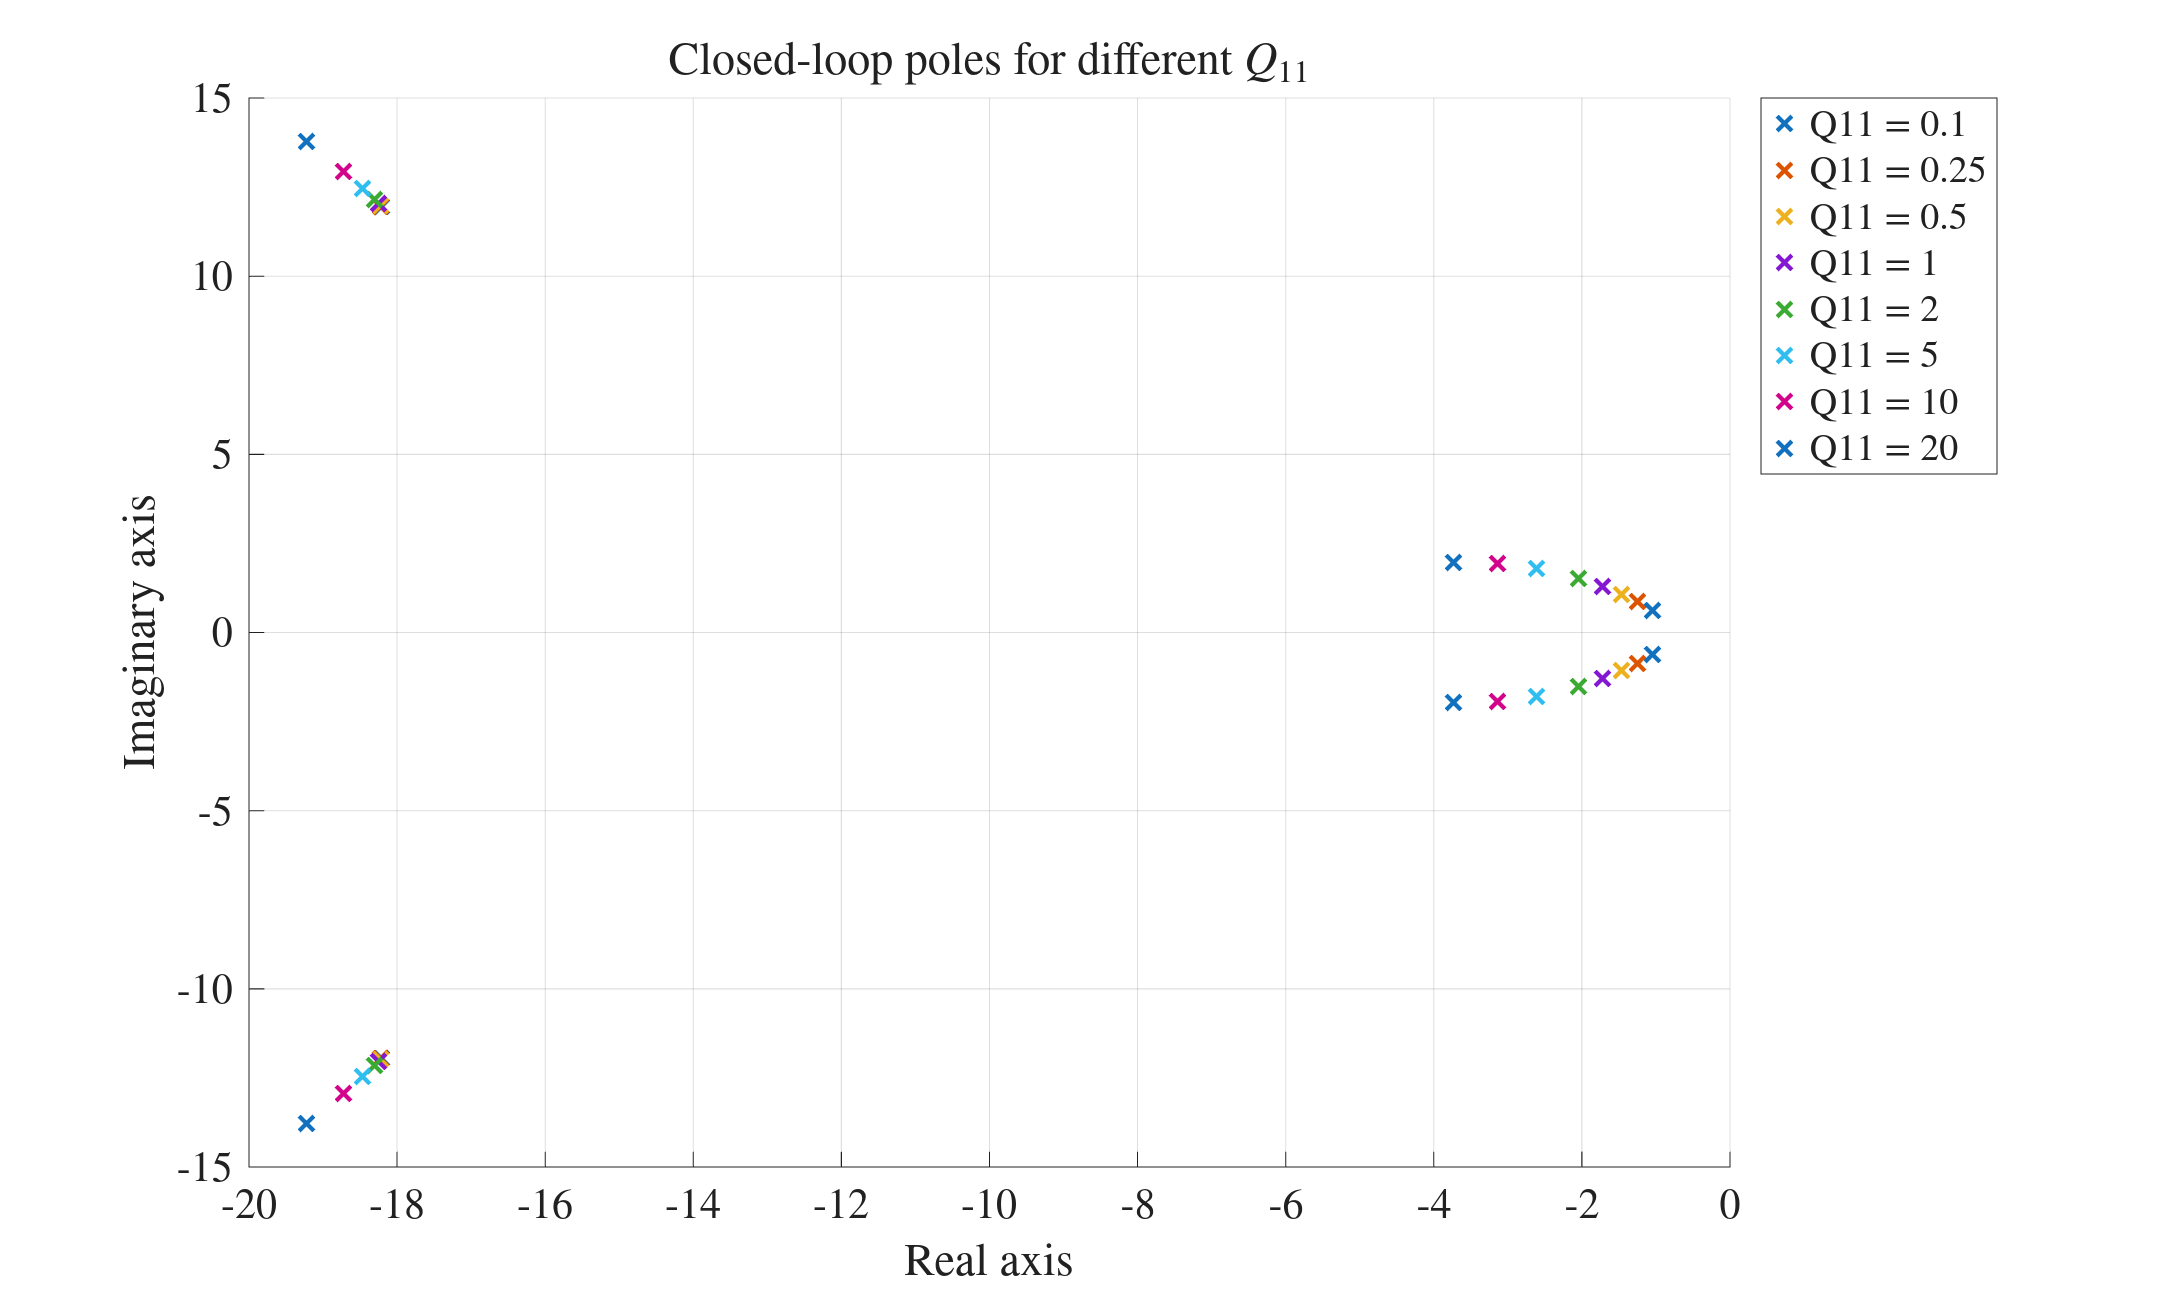
\includegraphics[width=\linewidth]{figures/q11_poles.png}
    \caption{Poles of the system.}
  \end{subfigure}
  \caption{Simulation results for different values of $Q_{1,1}$.}
  \label{fig:q11}
\end{figure} 

\begin{figure}[htbp]
  \centering
  \begin{subfigure}{0.45\textwidth}
    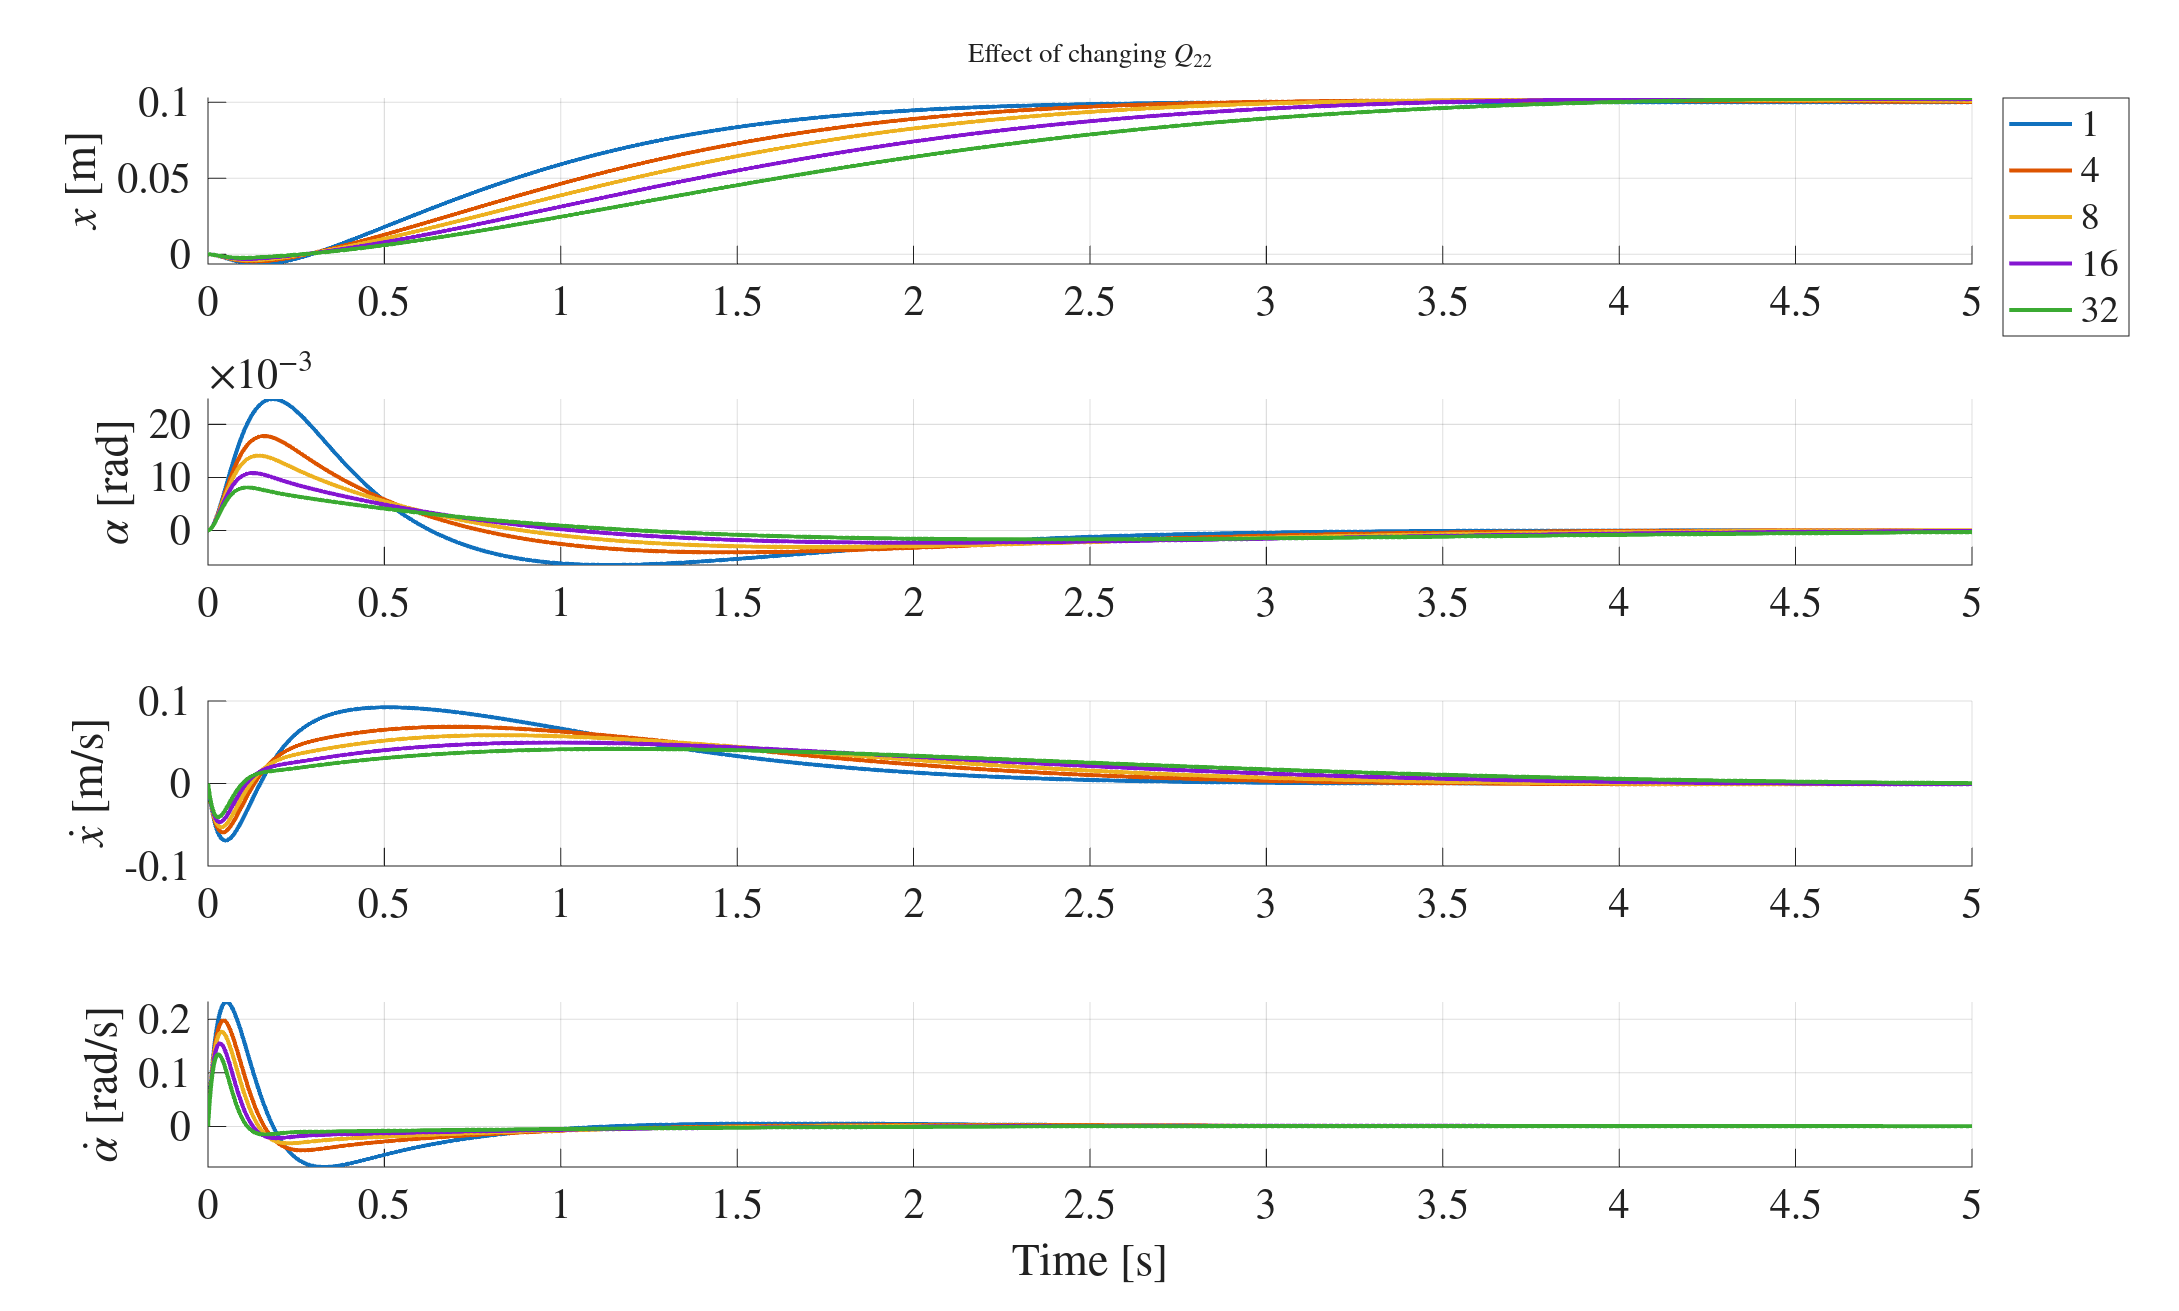
\includegraphics[width=\linewidth]{figures/q22_states.png}
    \caption{States evolution.}
  \end{subfigure}
  \begin{subfigure}{0.45\textwidth}
    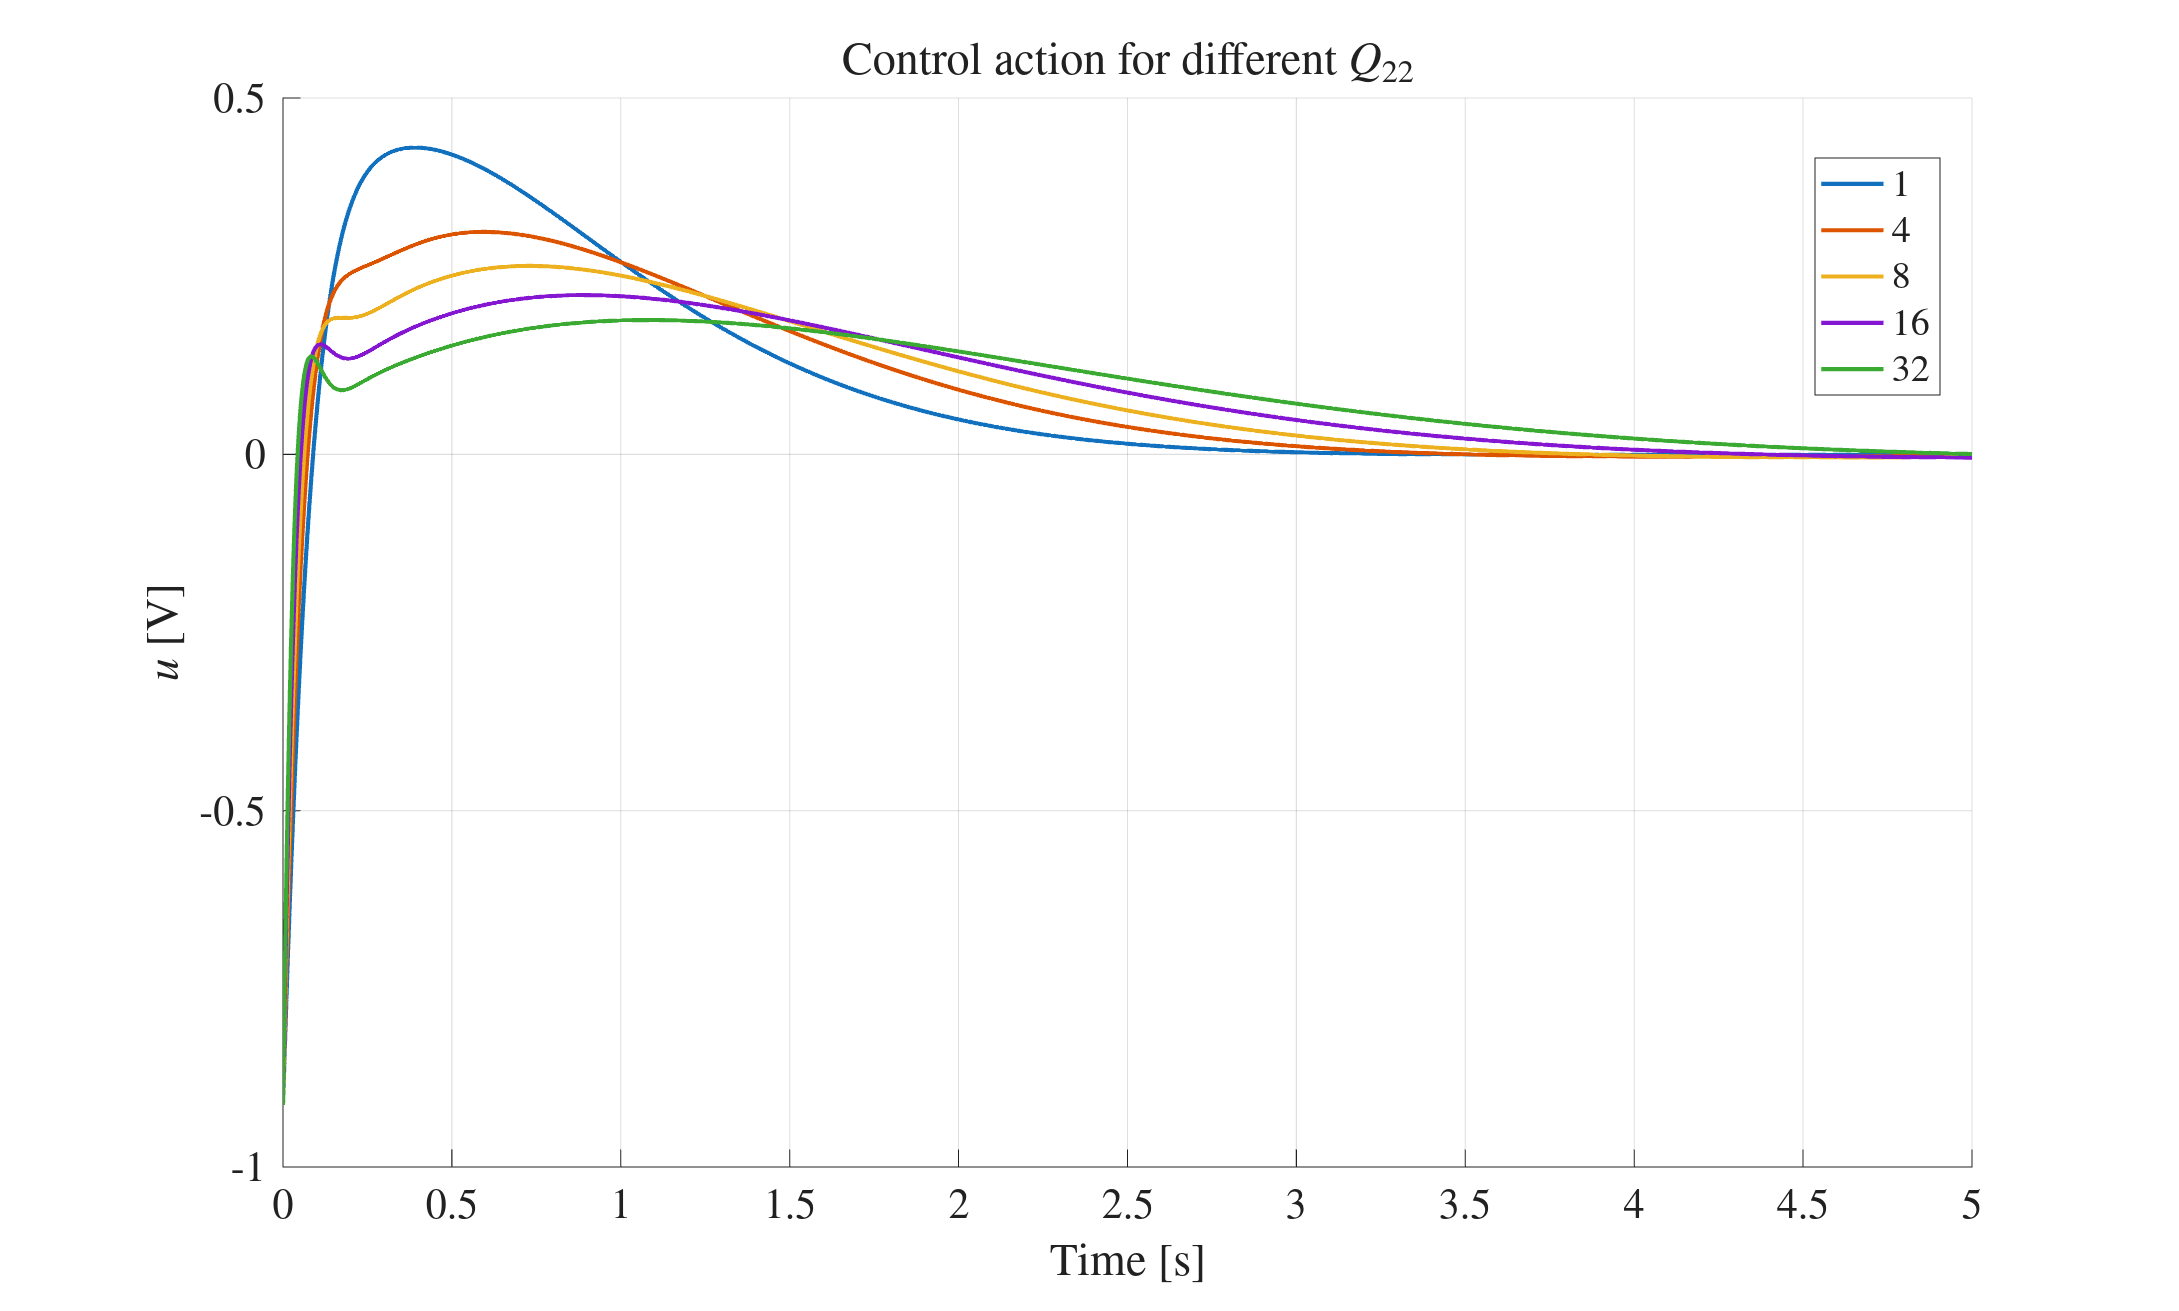
\includegraphics[width=\linewidth]{figures/q22_voltage.png}
    \caption{Control action evolution.}
  \end{subfigure}
  \begin{subfigure}{0.45\textwidth}
    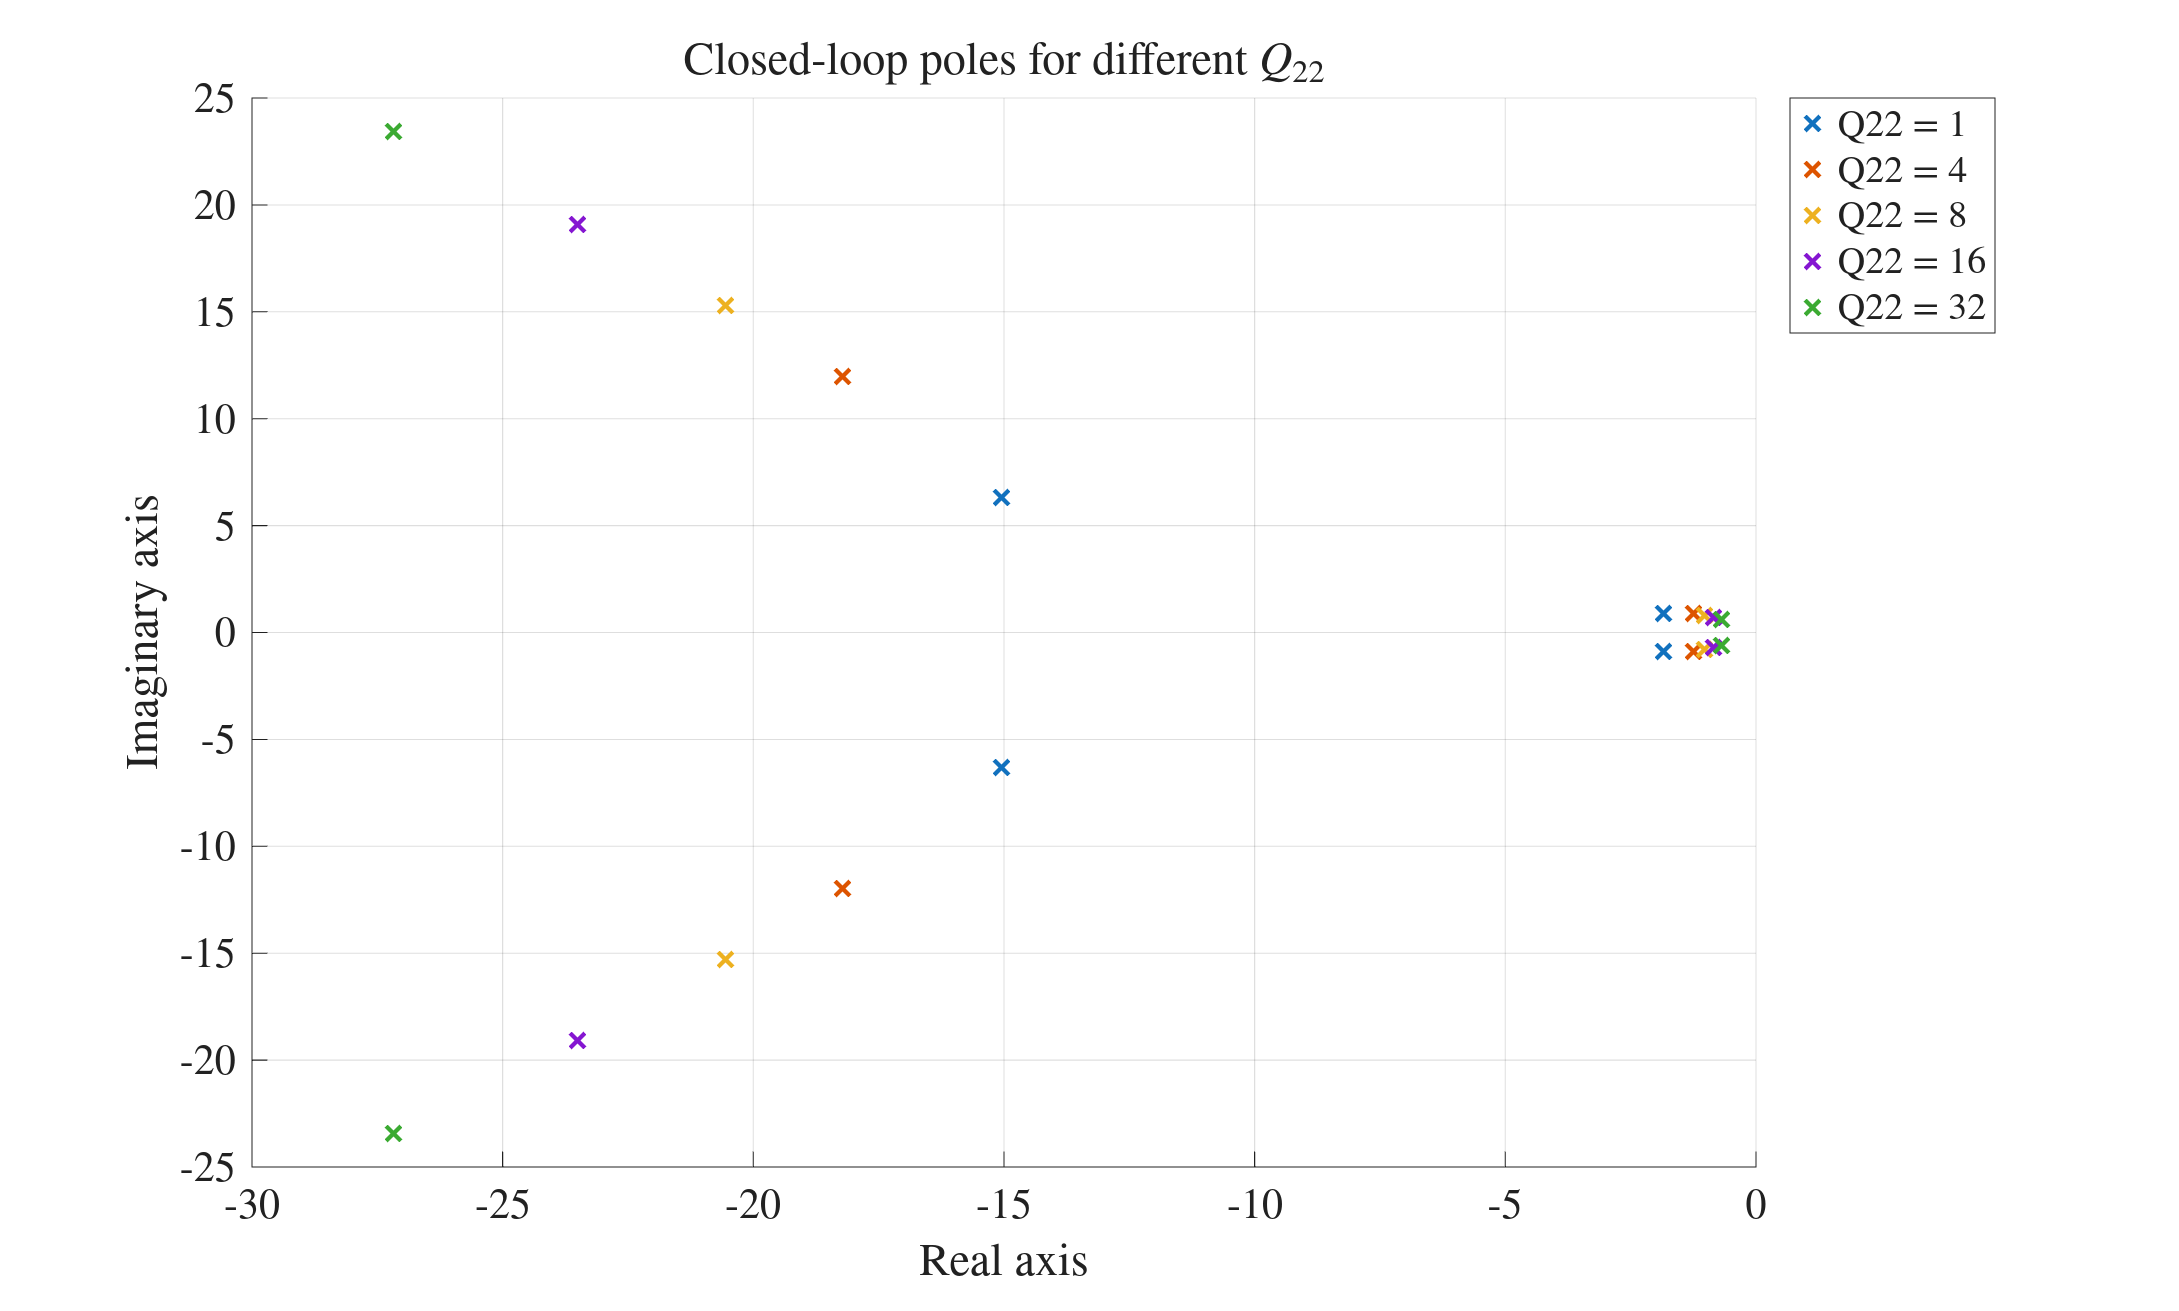
\includegraphics[width=\linewidth]{figures/q22_poles.png}
    \caption{Poles of the system.}
  \end{subfigure}
  \caption{Simulation results for different values of $Q_{2,2}$.}
  \label{fig:q22}
\end{figure} 

\begin{figure}[htbp]
  \centering
  \begin{subfigure}{0.45\textwidth}
    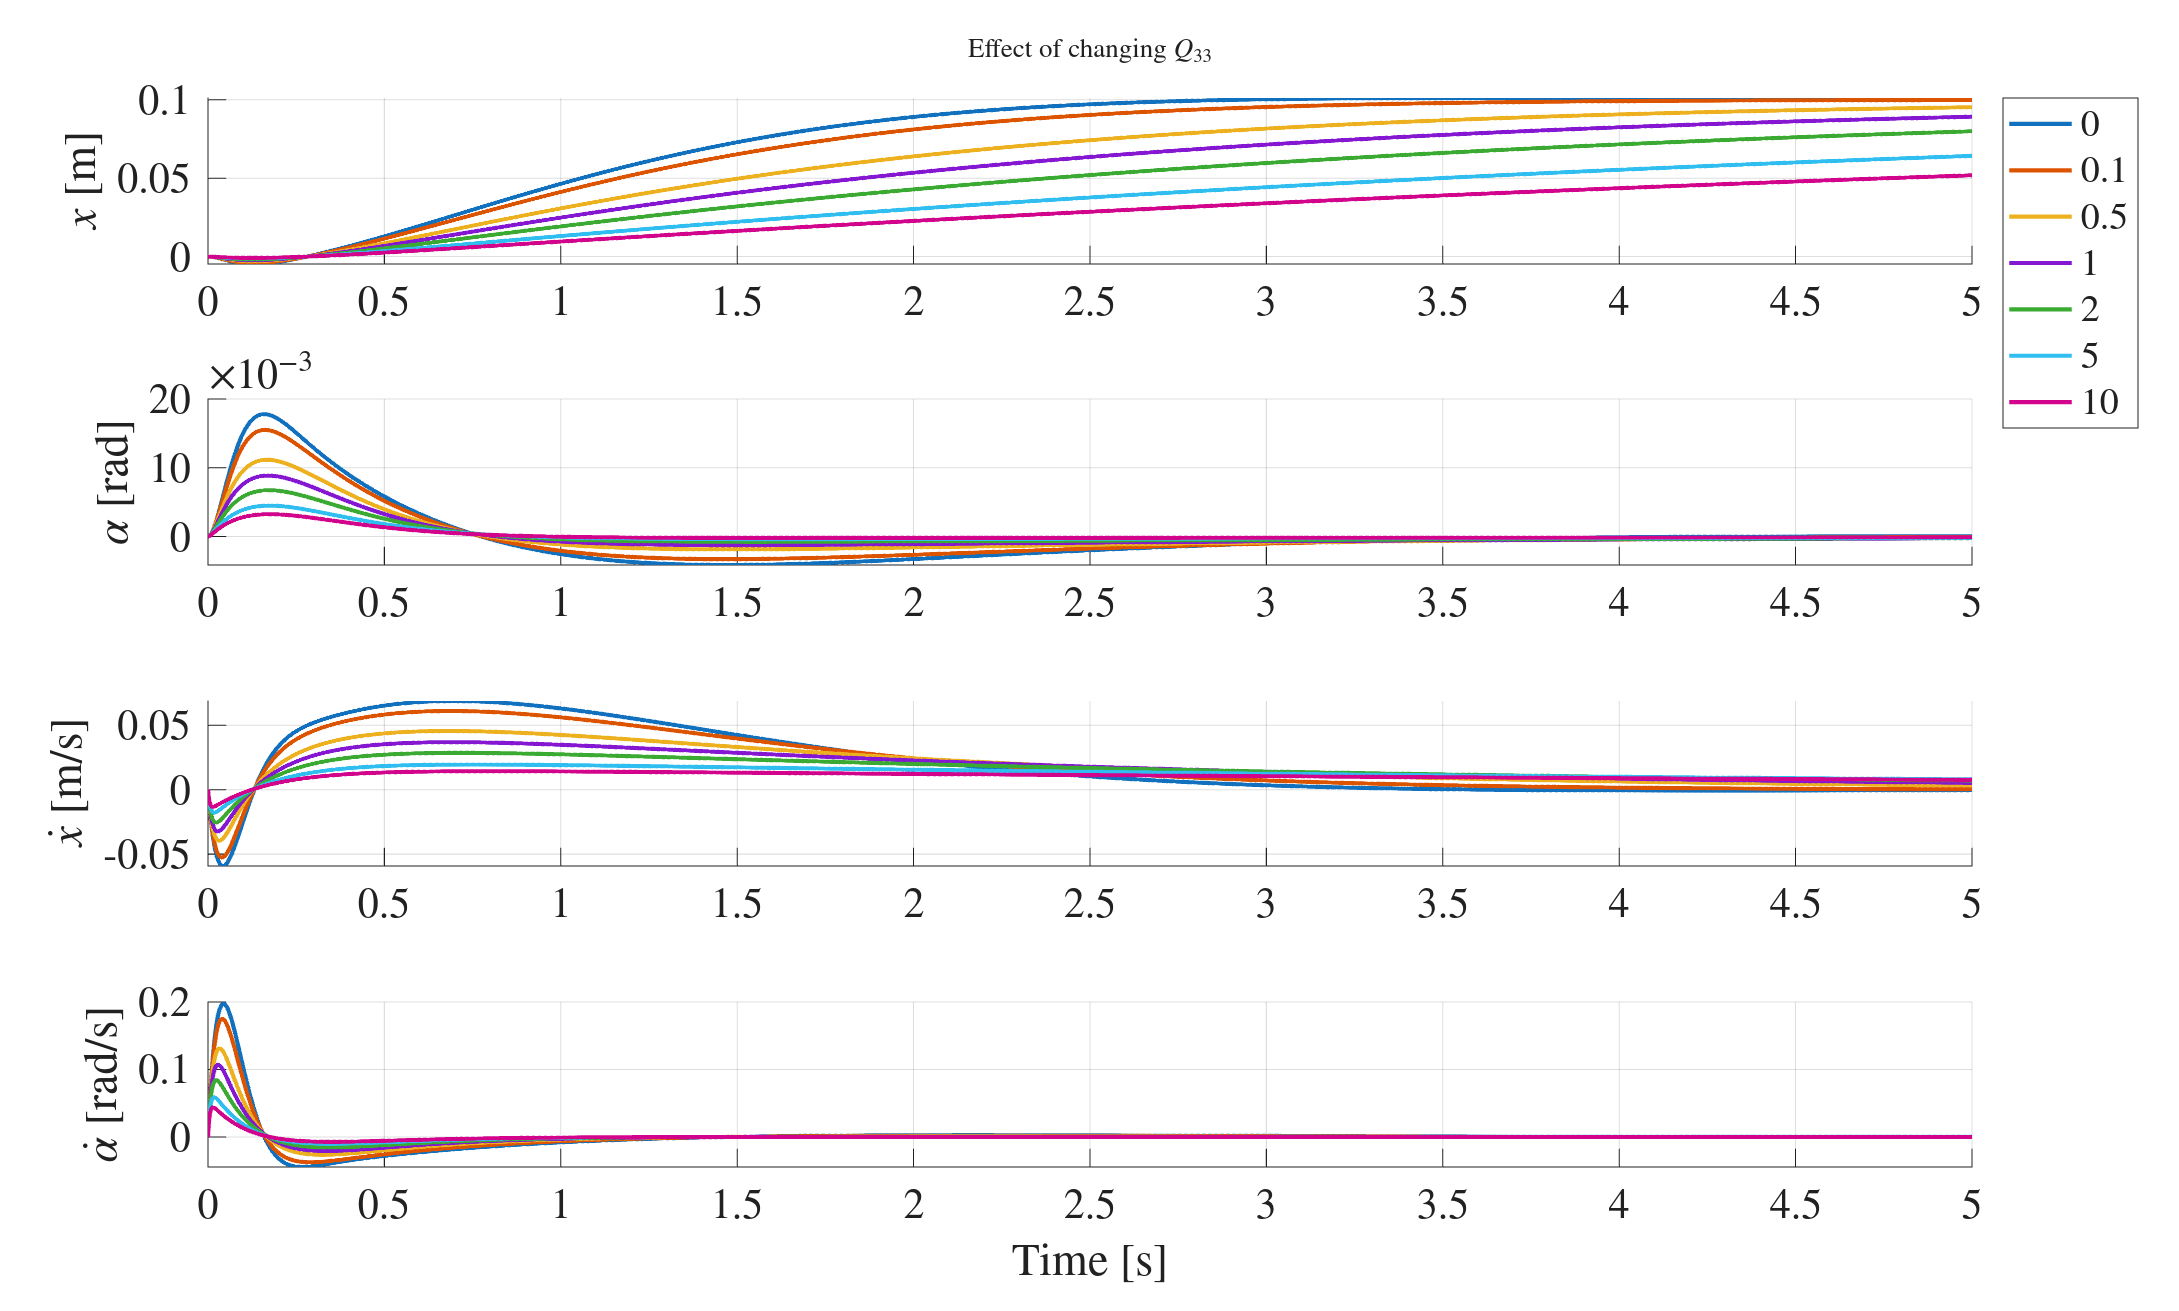
\includegraphics[width=\linewidth]{figures/q33_states.png}
    \caption{States evolution.}
  \end{subfigure}
  \begin{subfigure}{0.45\textwidth}
    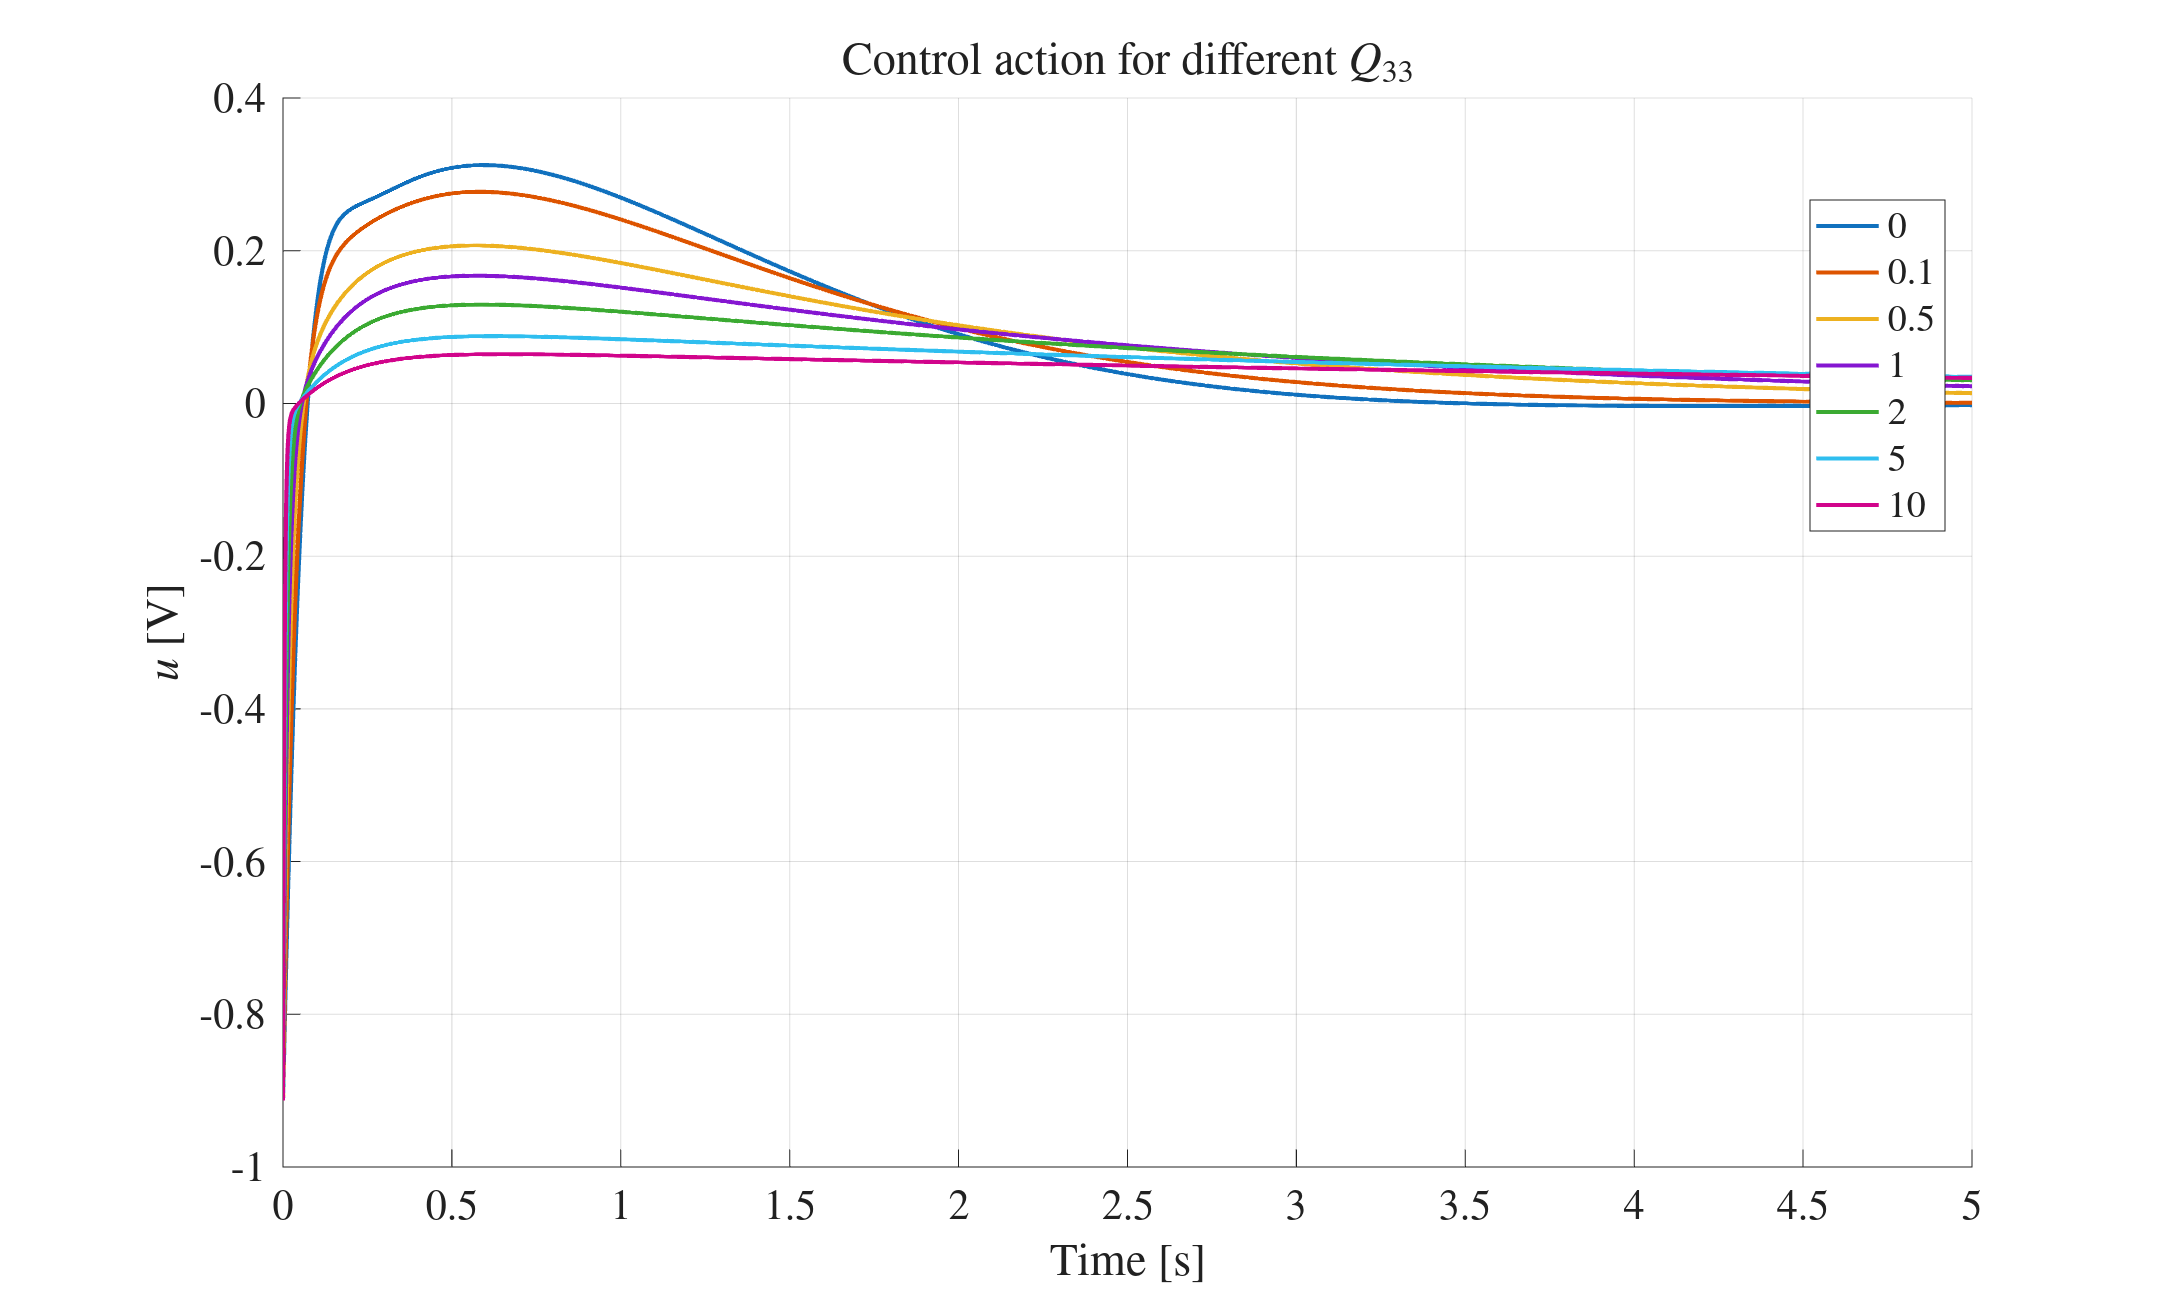
\includegraphics[width=\linewidth]{figures/q33_voltage.png}
    \caption{Control action evolution.}
  \end{subfigure}
  \begin{subfigure}{0.45\textwidth}
    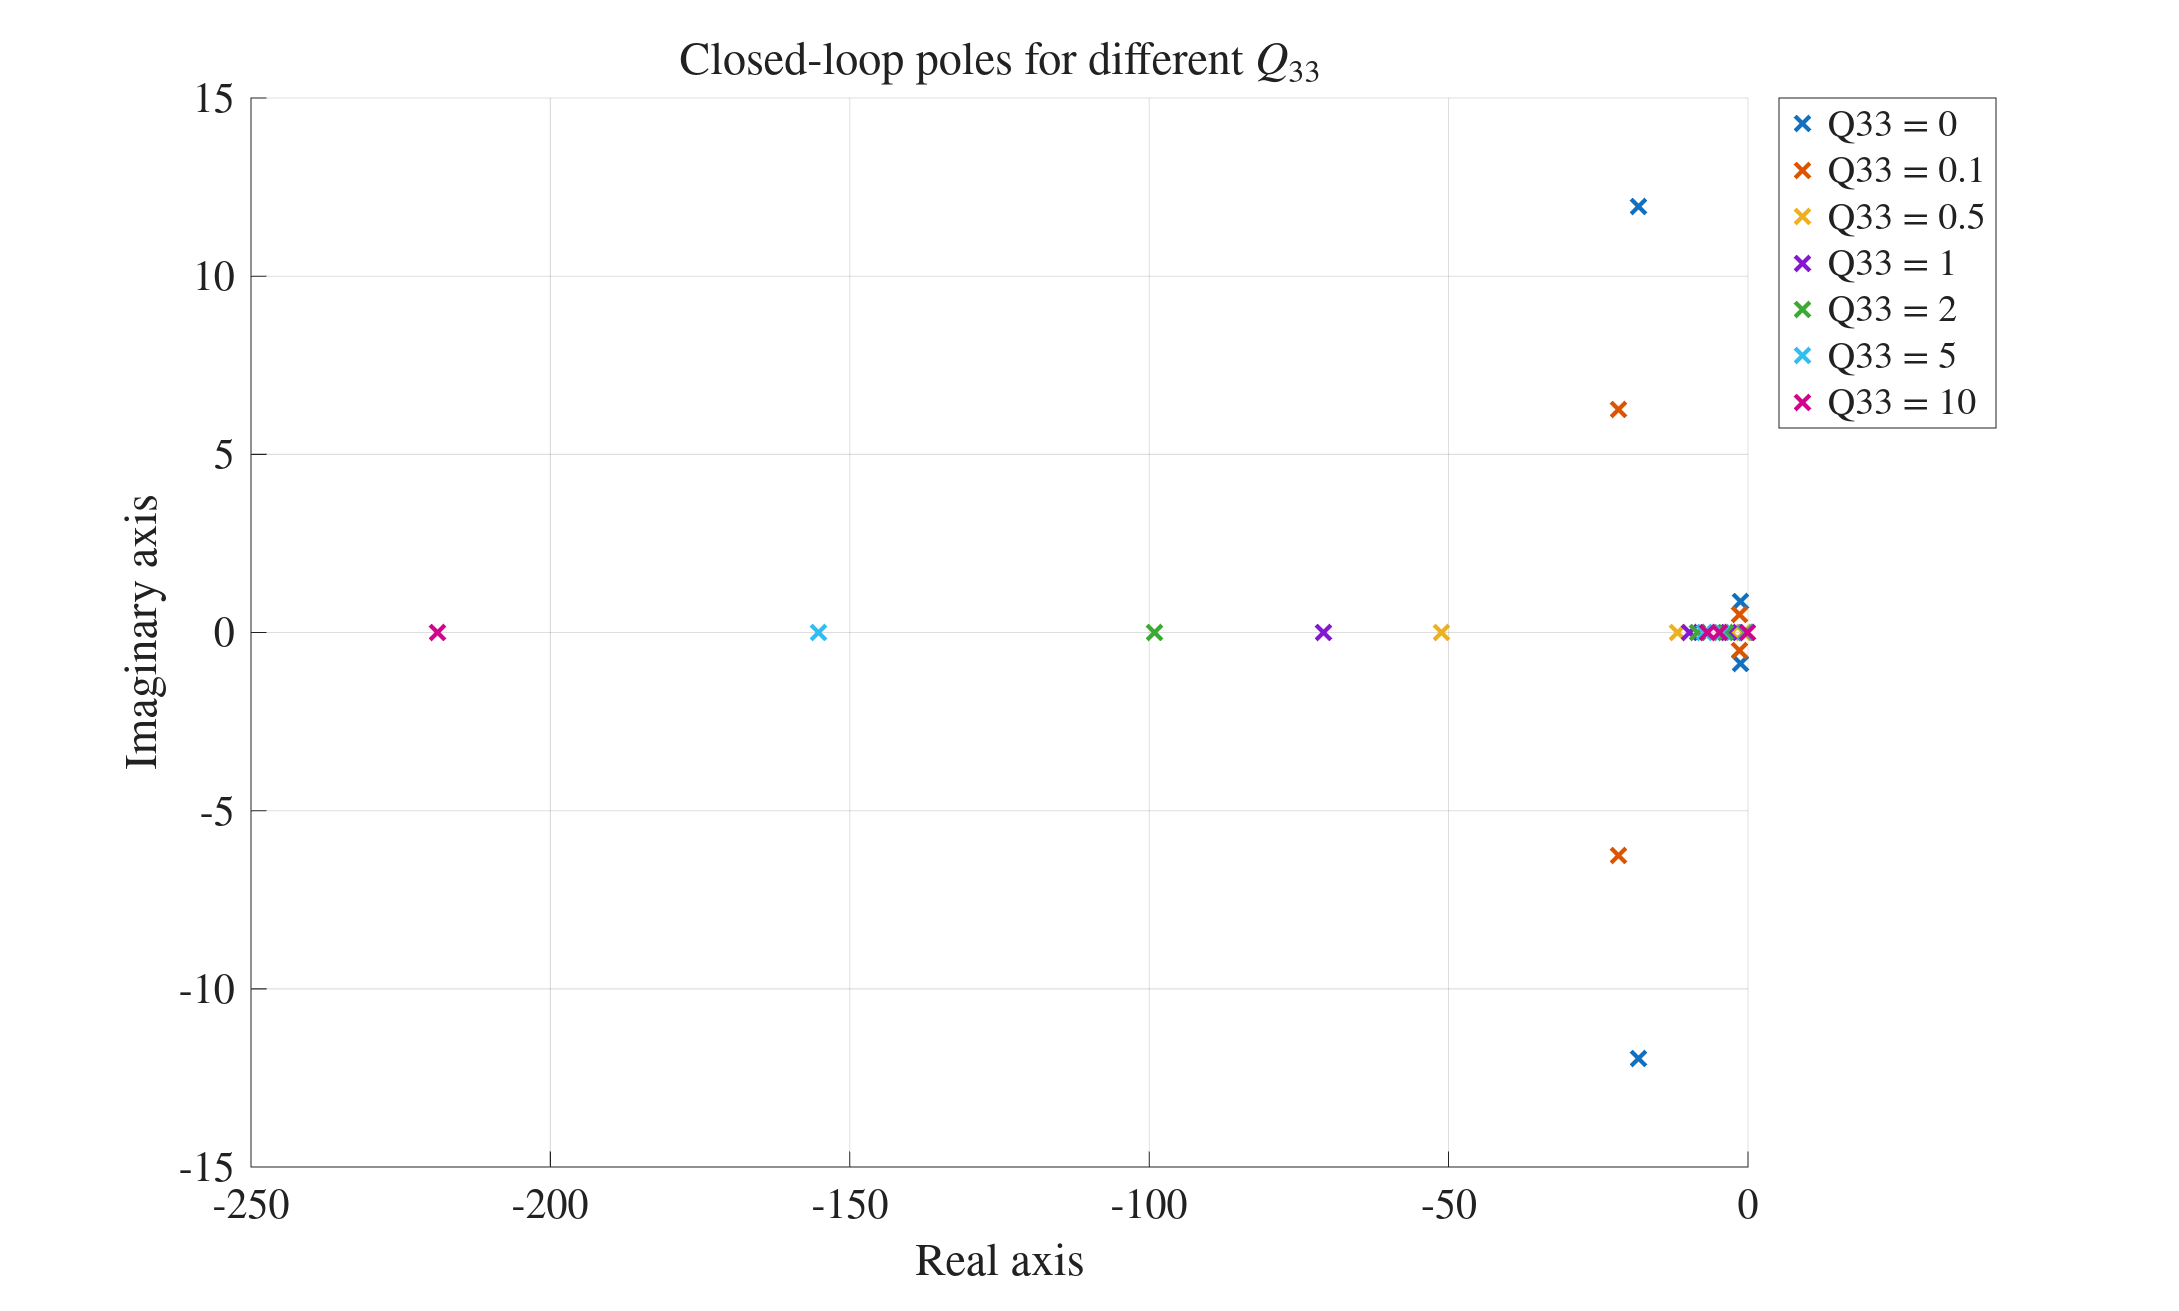
\includegraphics[width=\linewidth]{figures/q33_poles.png}
    \caption{Poles of the system.}
  \end{subfigure}
  \caption{Simulation results for different values of $Q_{3,3}$.}
  \label{fig:q33}
\end{figure} 

\begin{figure}[htbp]
  \centering
  \begin{subfigure}{0.45\textwidth}
    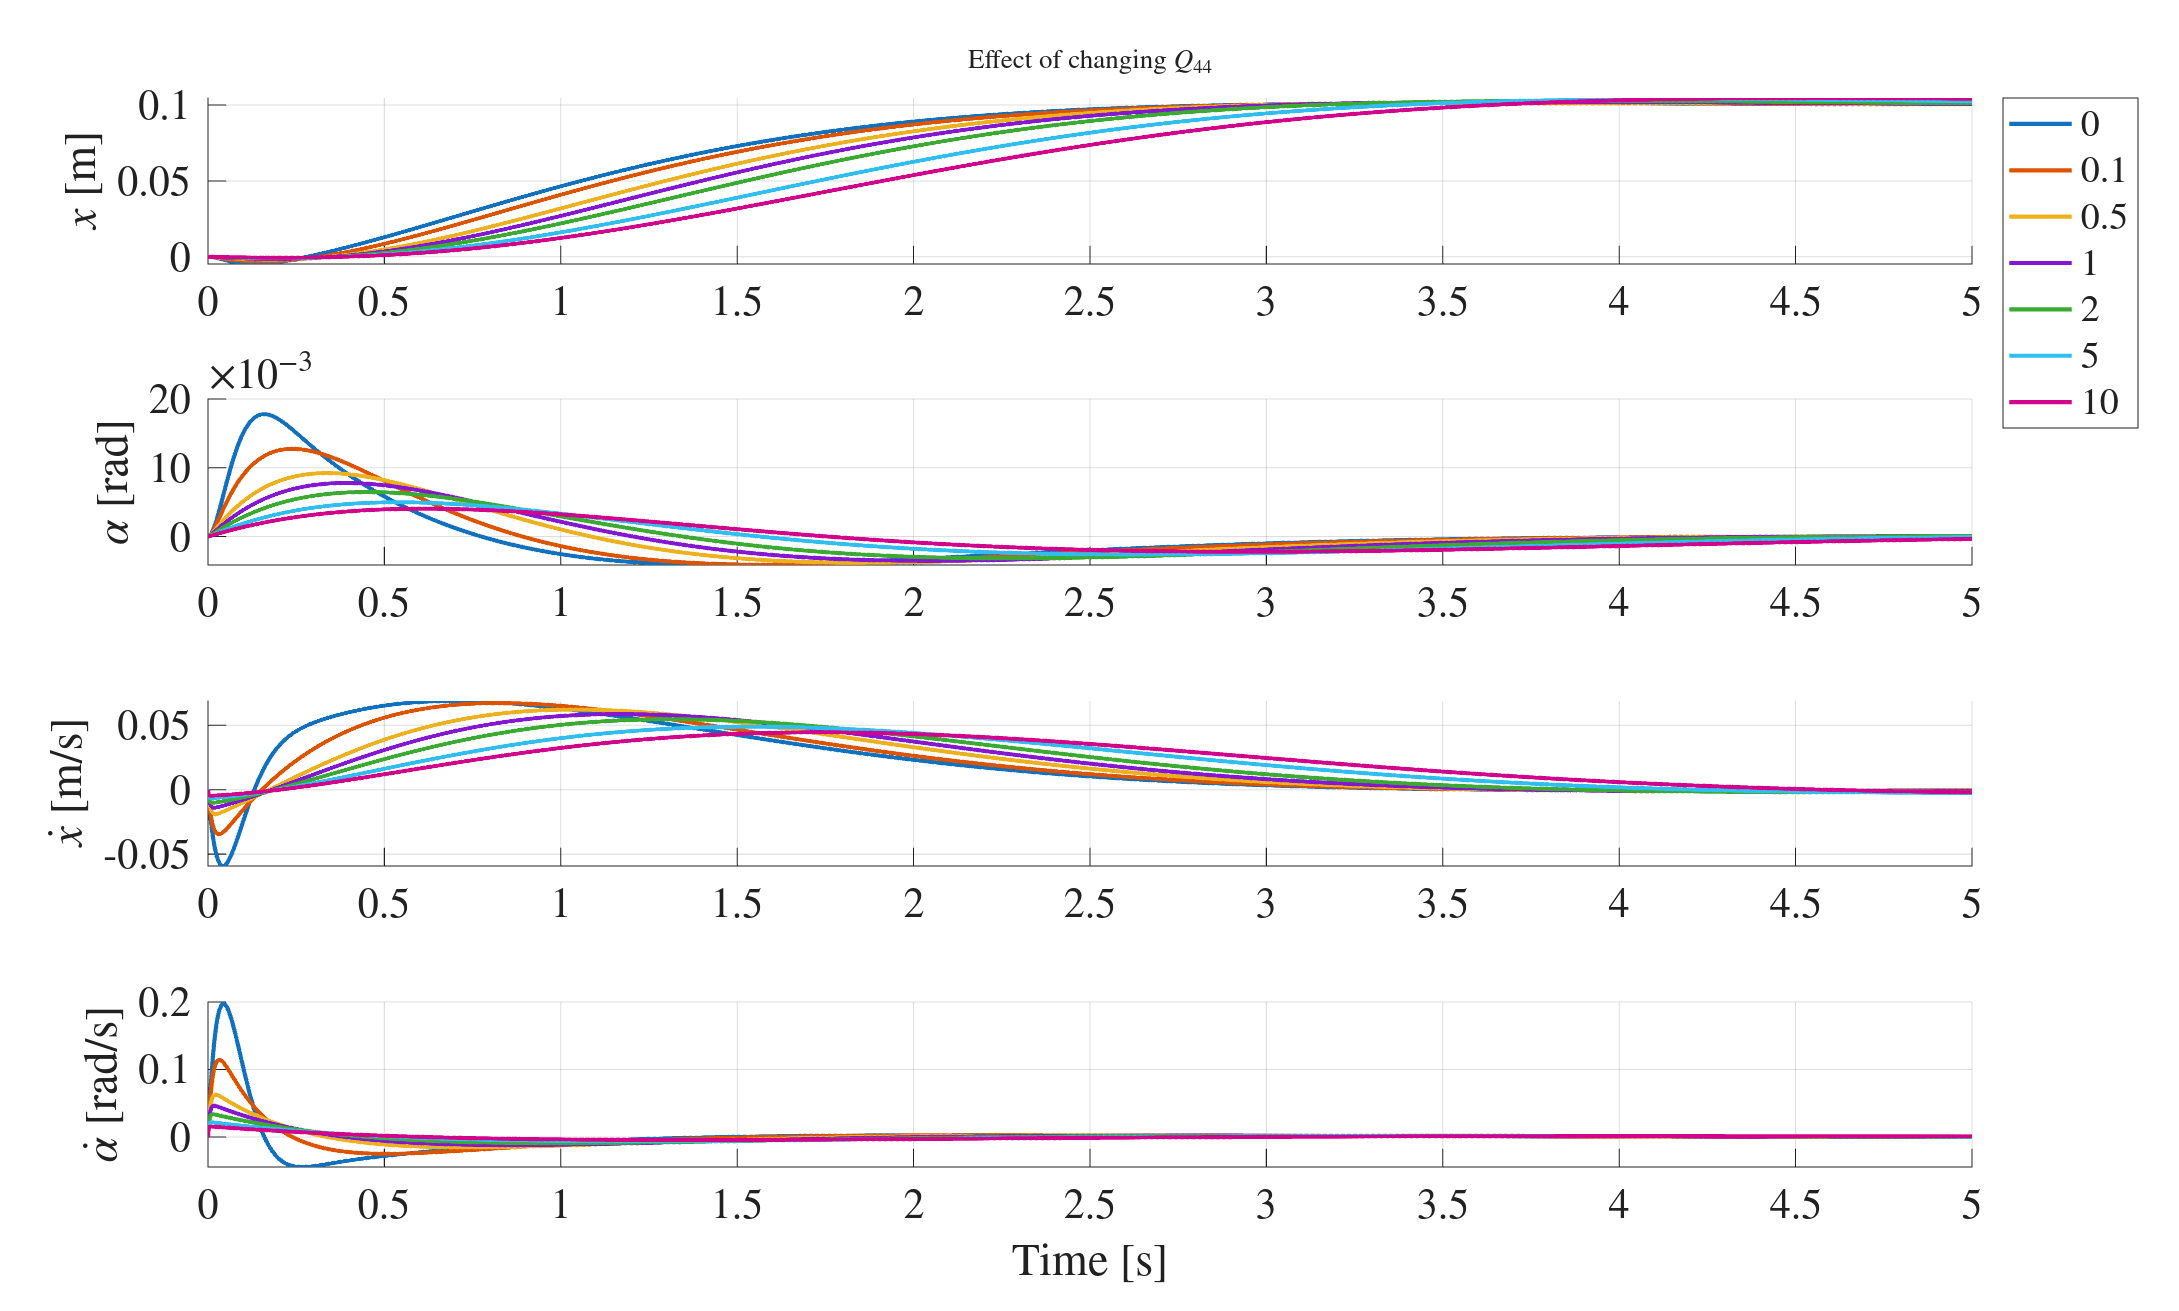
\includegraphics[width=\linewidth]{figures/q44_states.png}
    \caption{States evolution.}
  \end{subfigure}
  \begin{subfigure}{0.45\textwidth}
    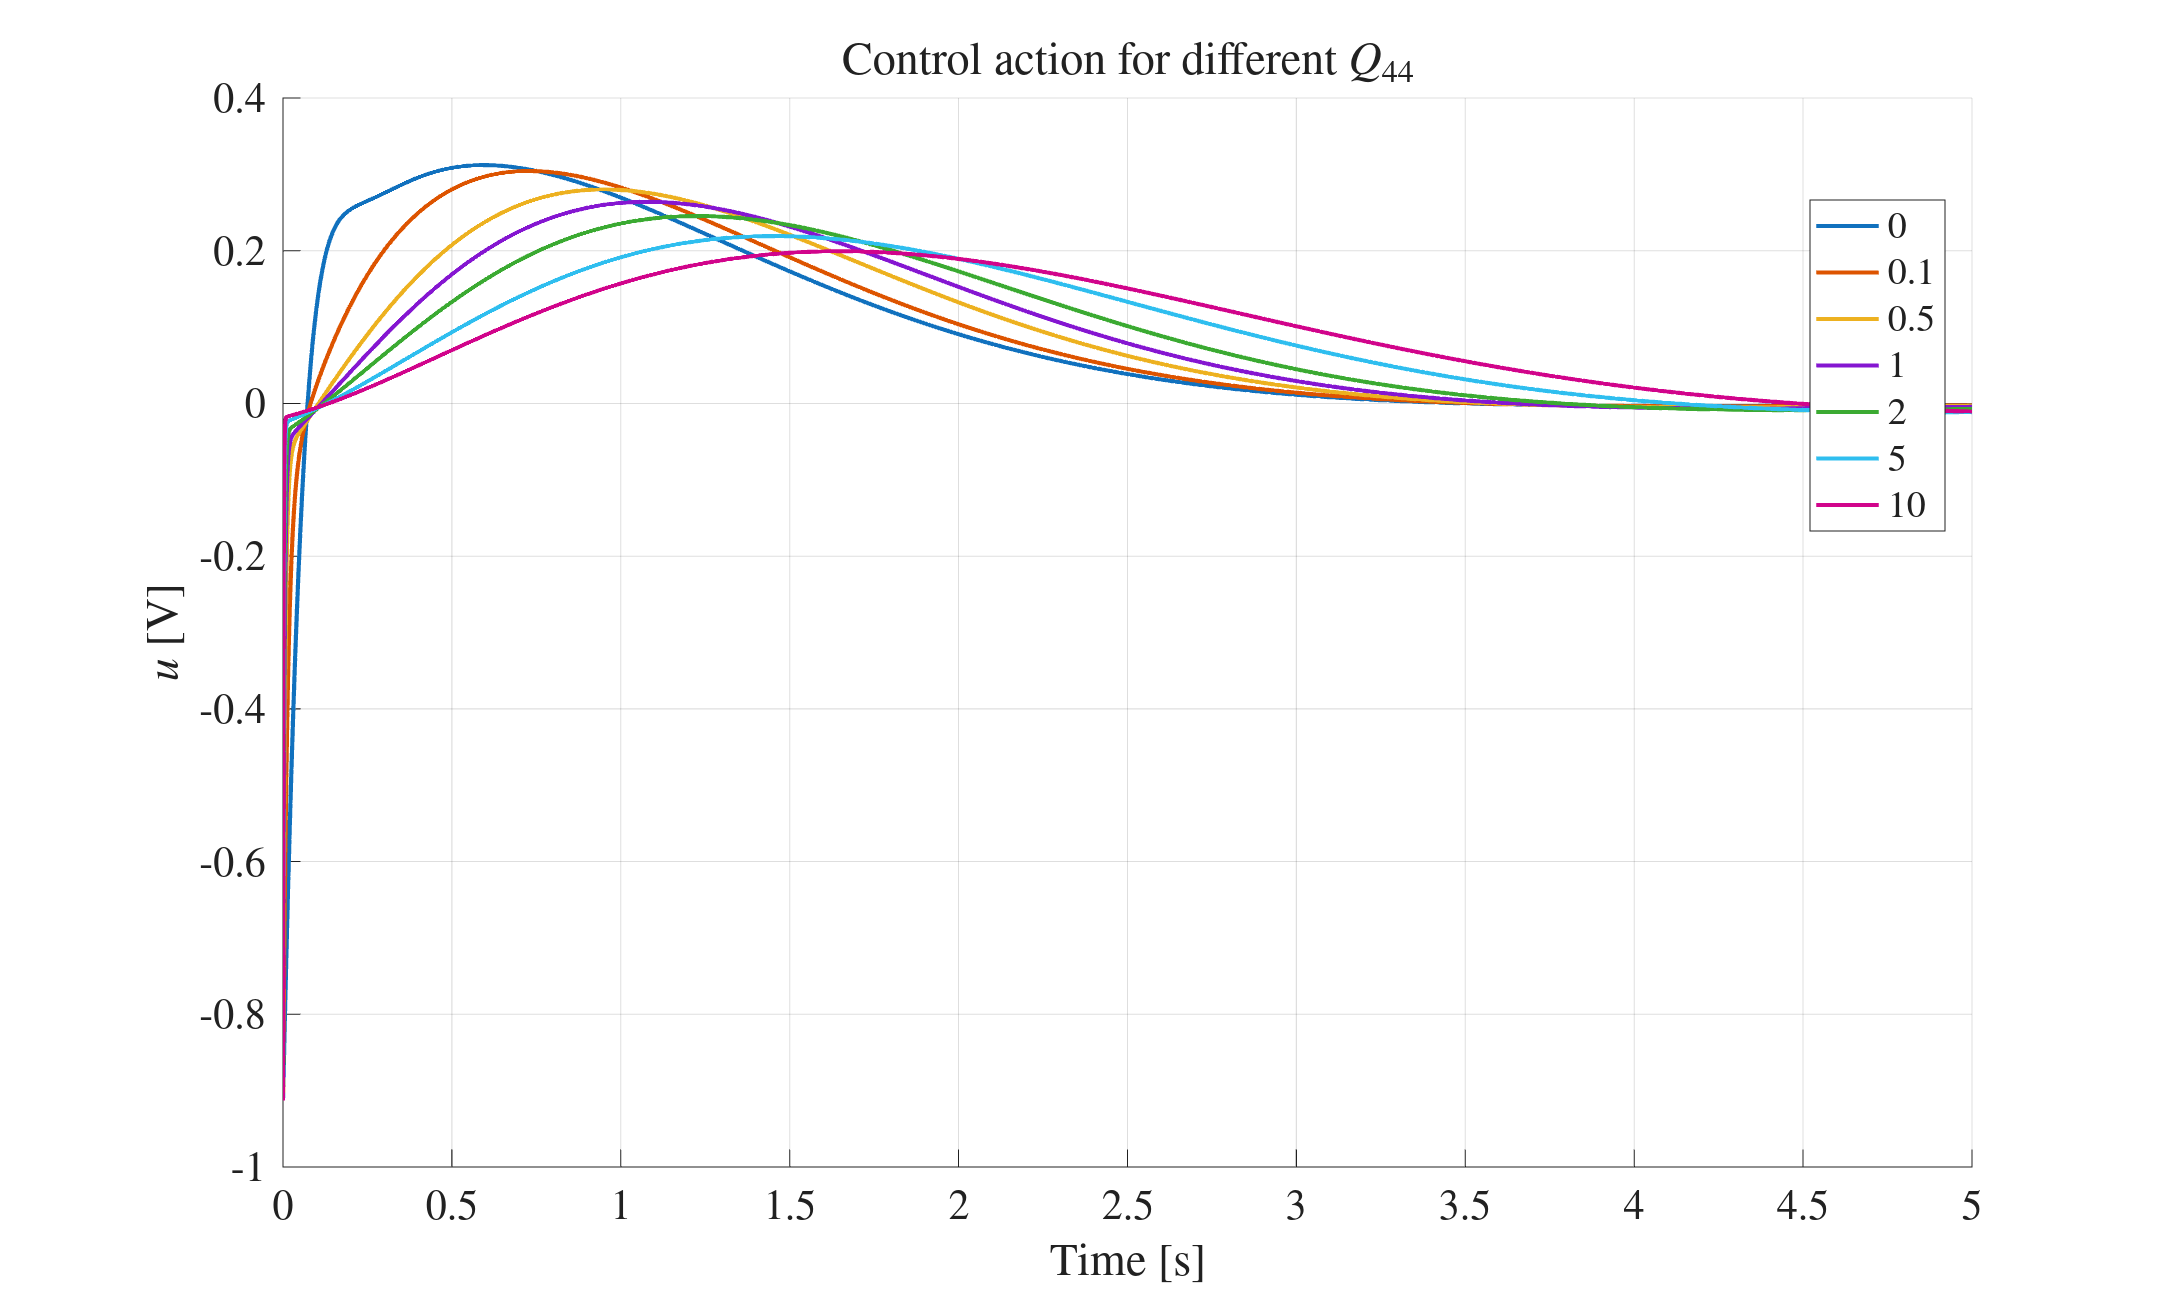
\includegraphics[width=\linewidth]{figures/q44_voltage.png}
    \caption{Control action evolution.}
  \end{subfigure}
  \begin{subfigure}{0.45\textwidth}
    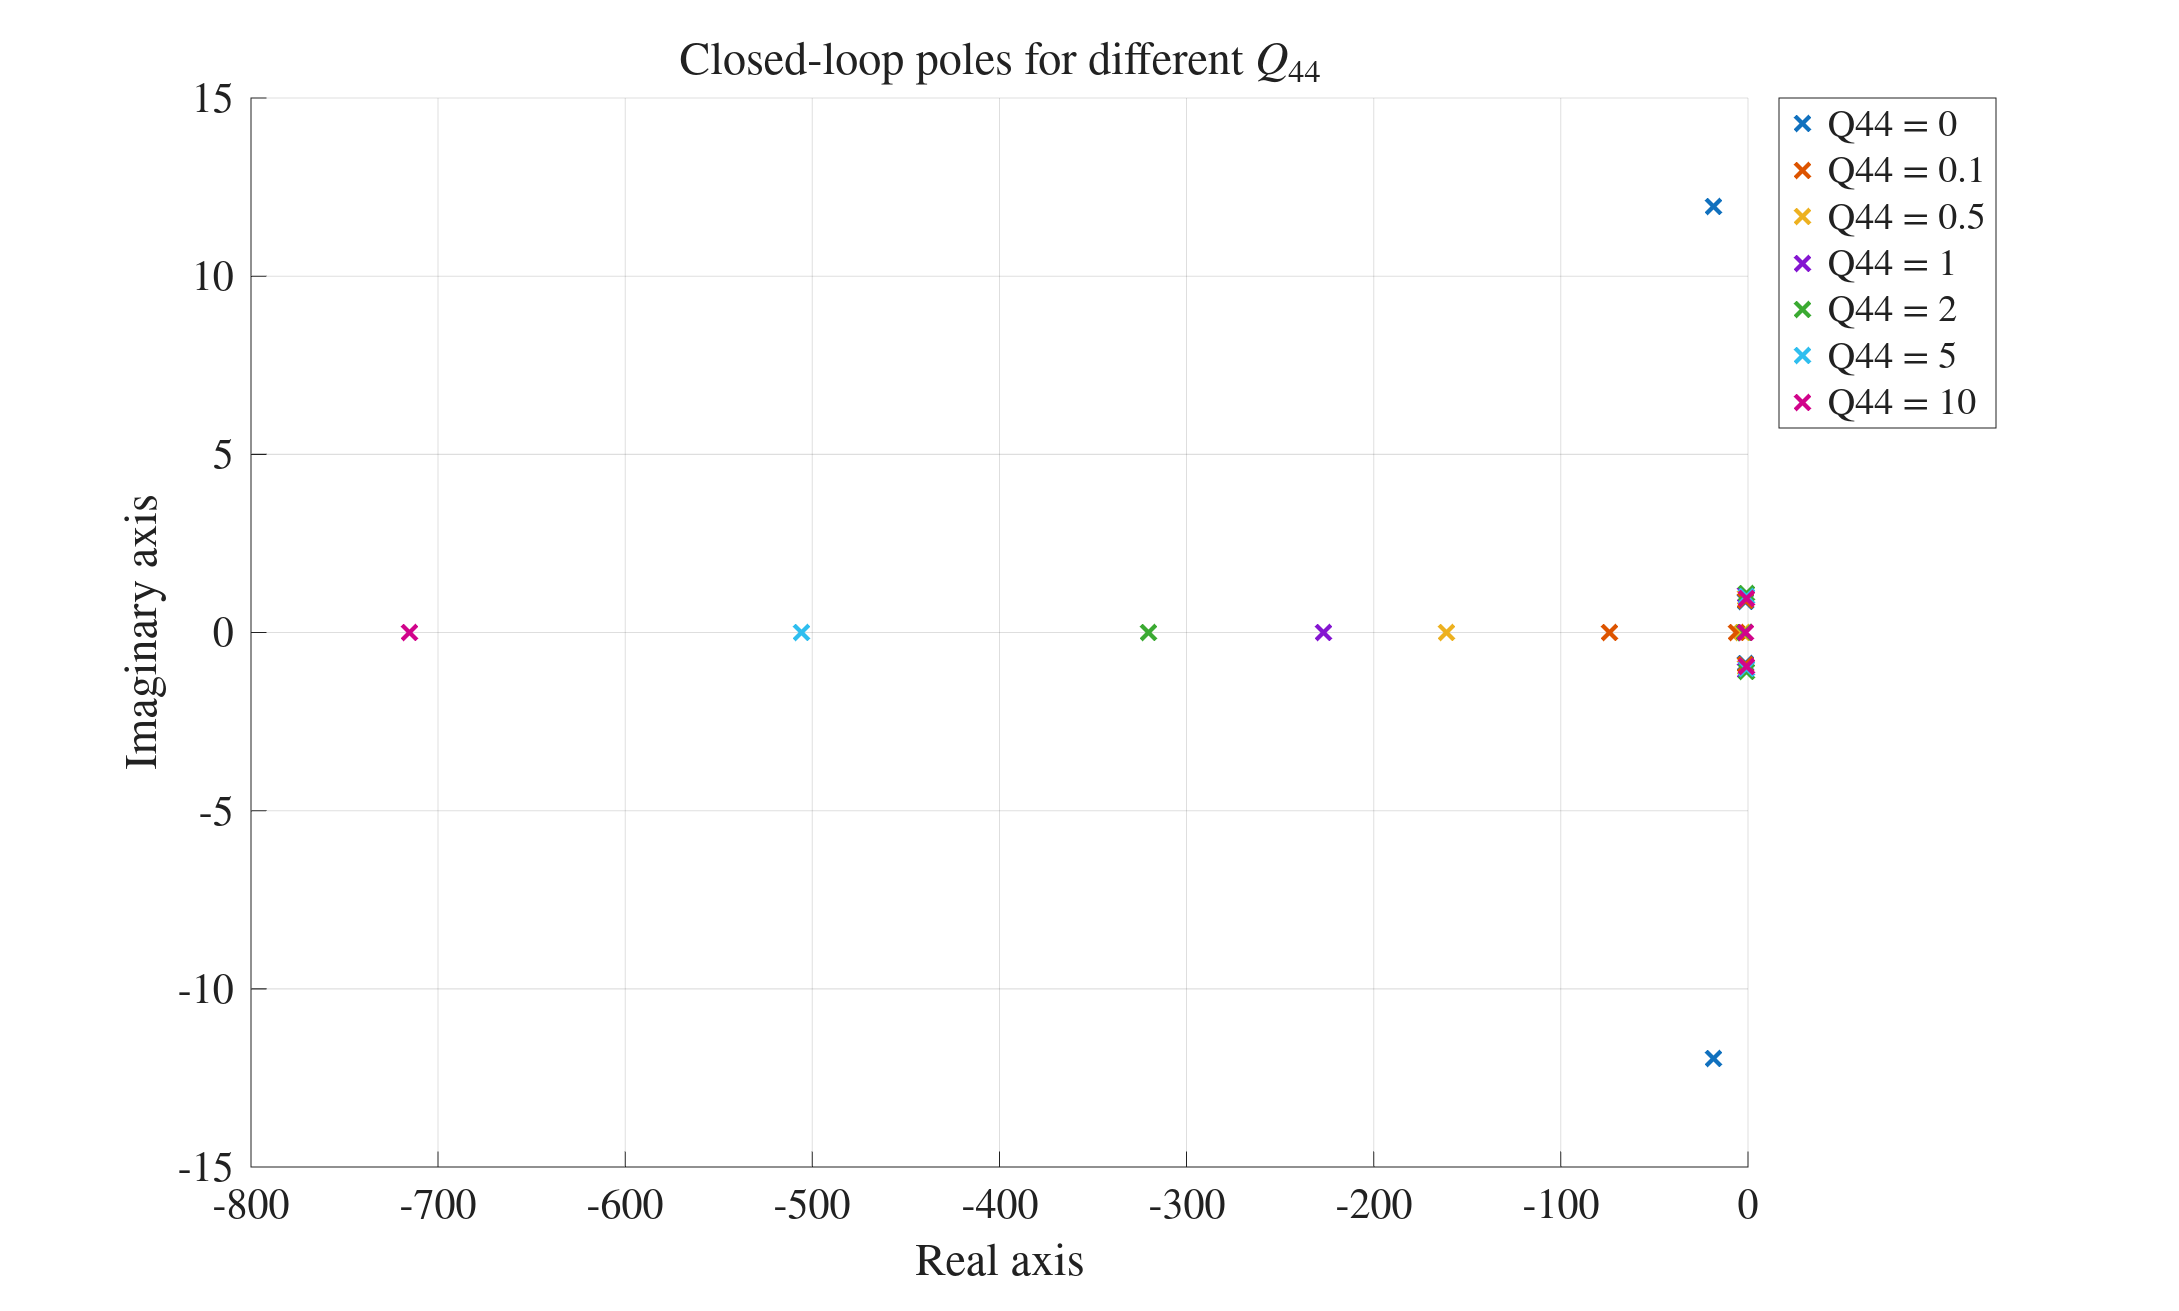
\includegraphics[width=\linewidth]{figures/q44_poles.png}
    \caption{Poles of the system.}
  \end{subfigure}
  \caption{Simulation results for different values of $Q_{4,4}$.}
  \label{fig:q44}
\end{figure} 

\begin{figure}[htbp]
  \centering
  \begin{subfigure}{0.45\textwidth}
    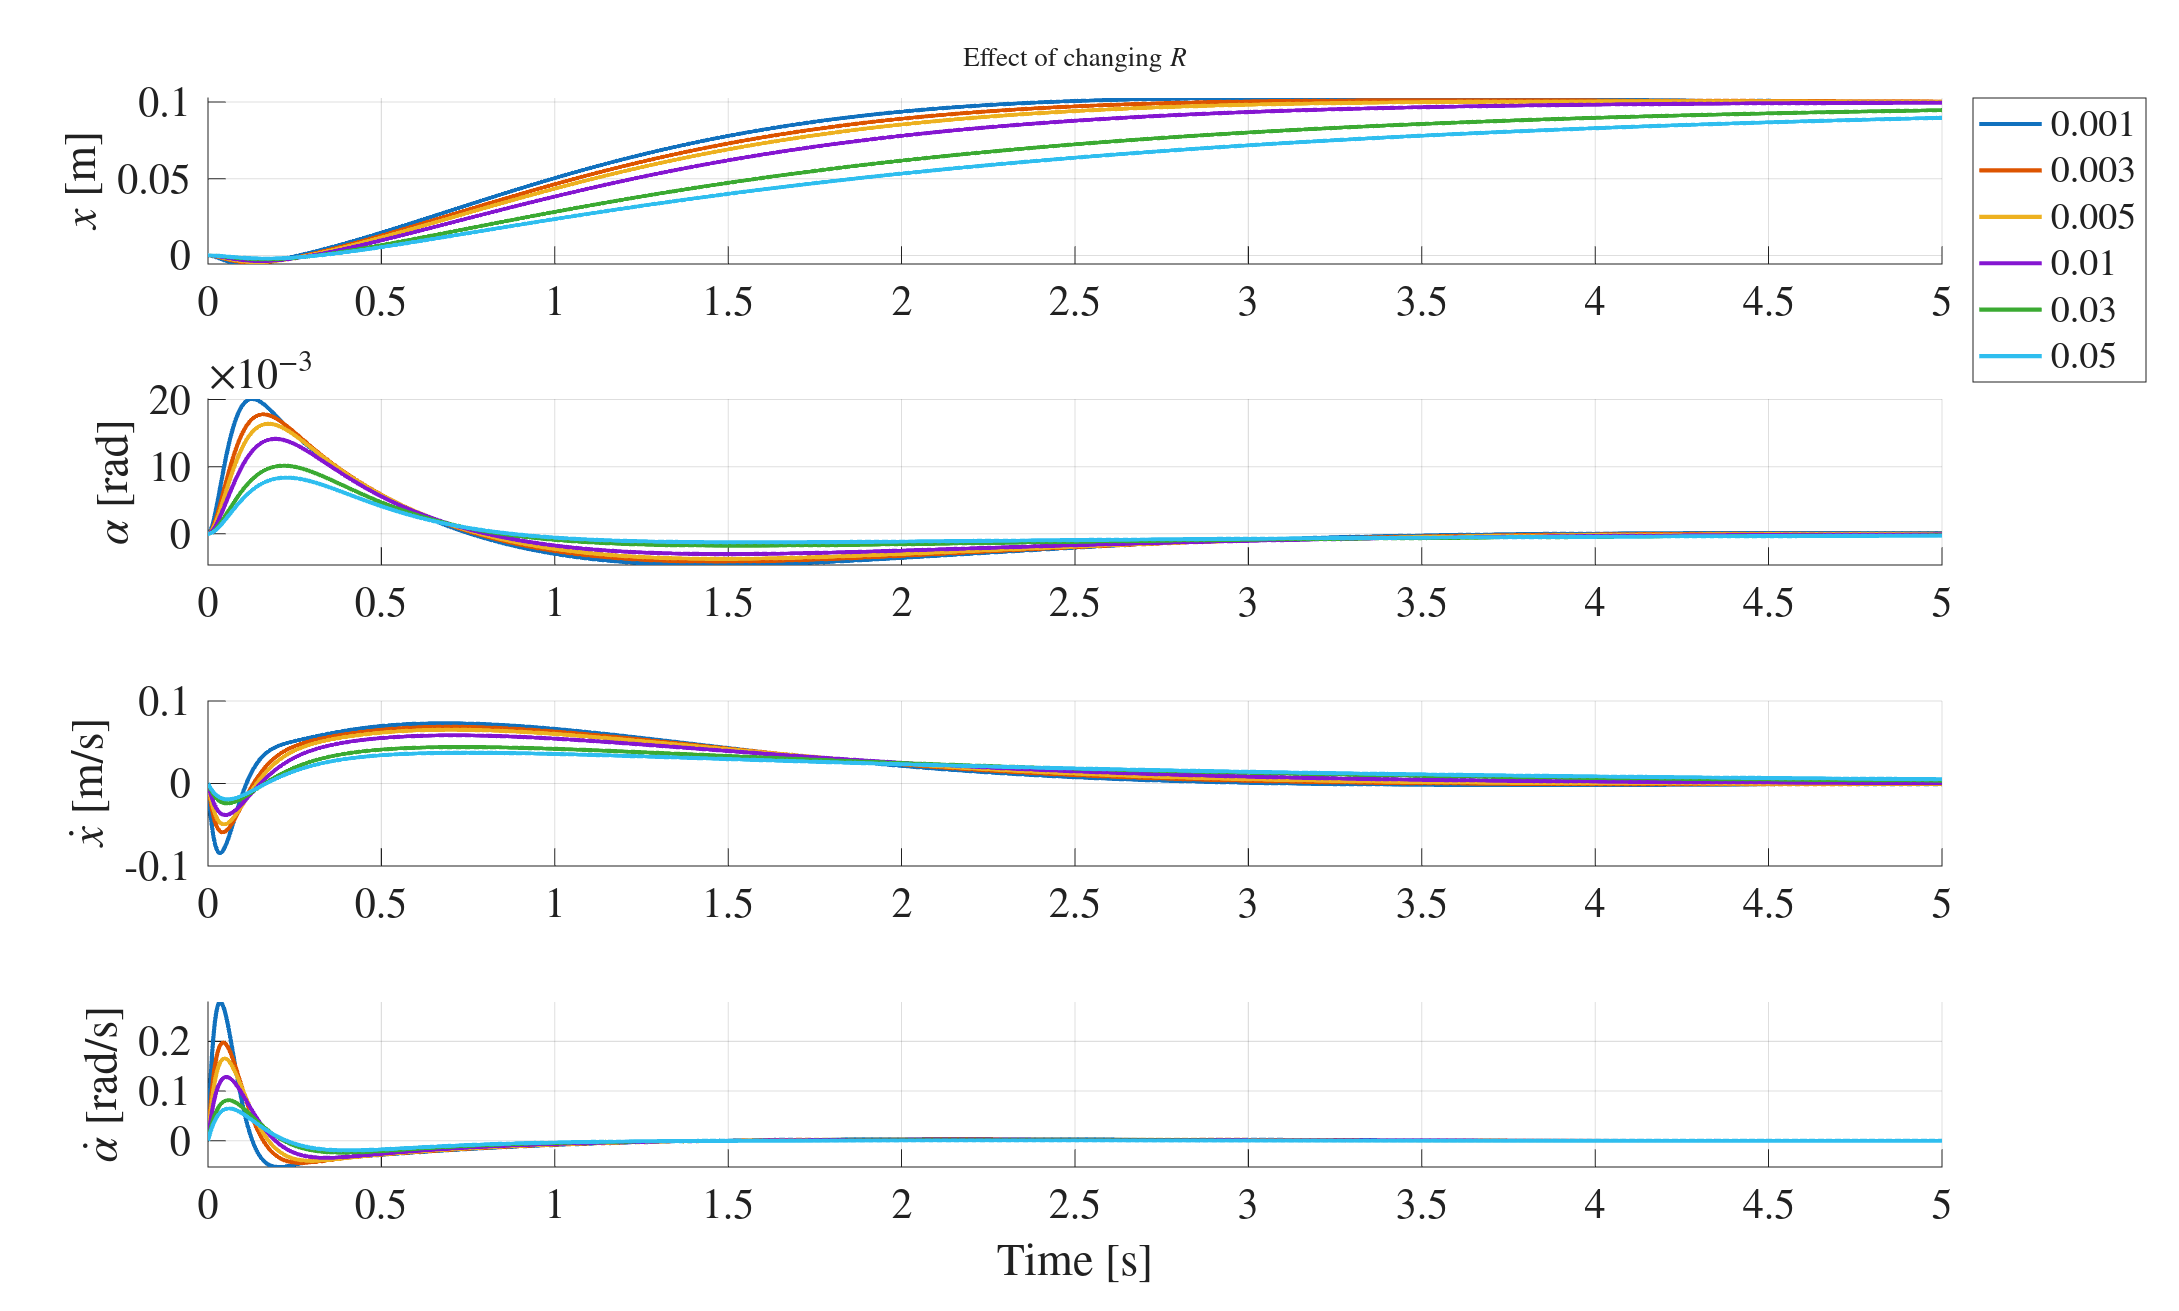
\includegraphics[width=\linewidth]{figures/r_states.png}
    \caption{States evolution.}
  \end{subfigure}
  \begin{subfigure}{0.45\textwidth}
    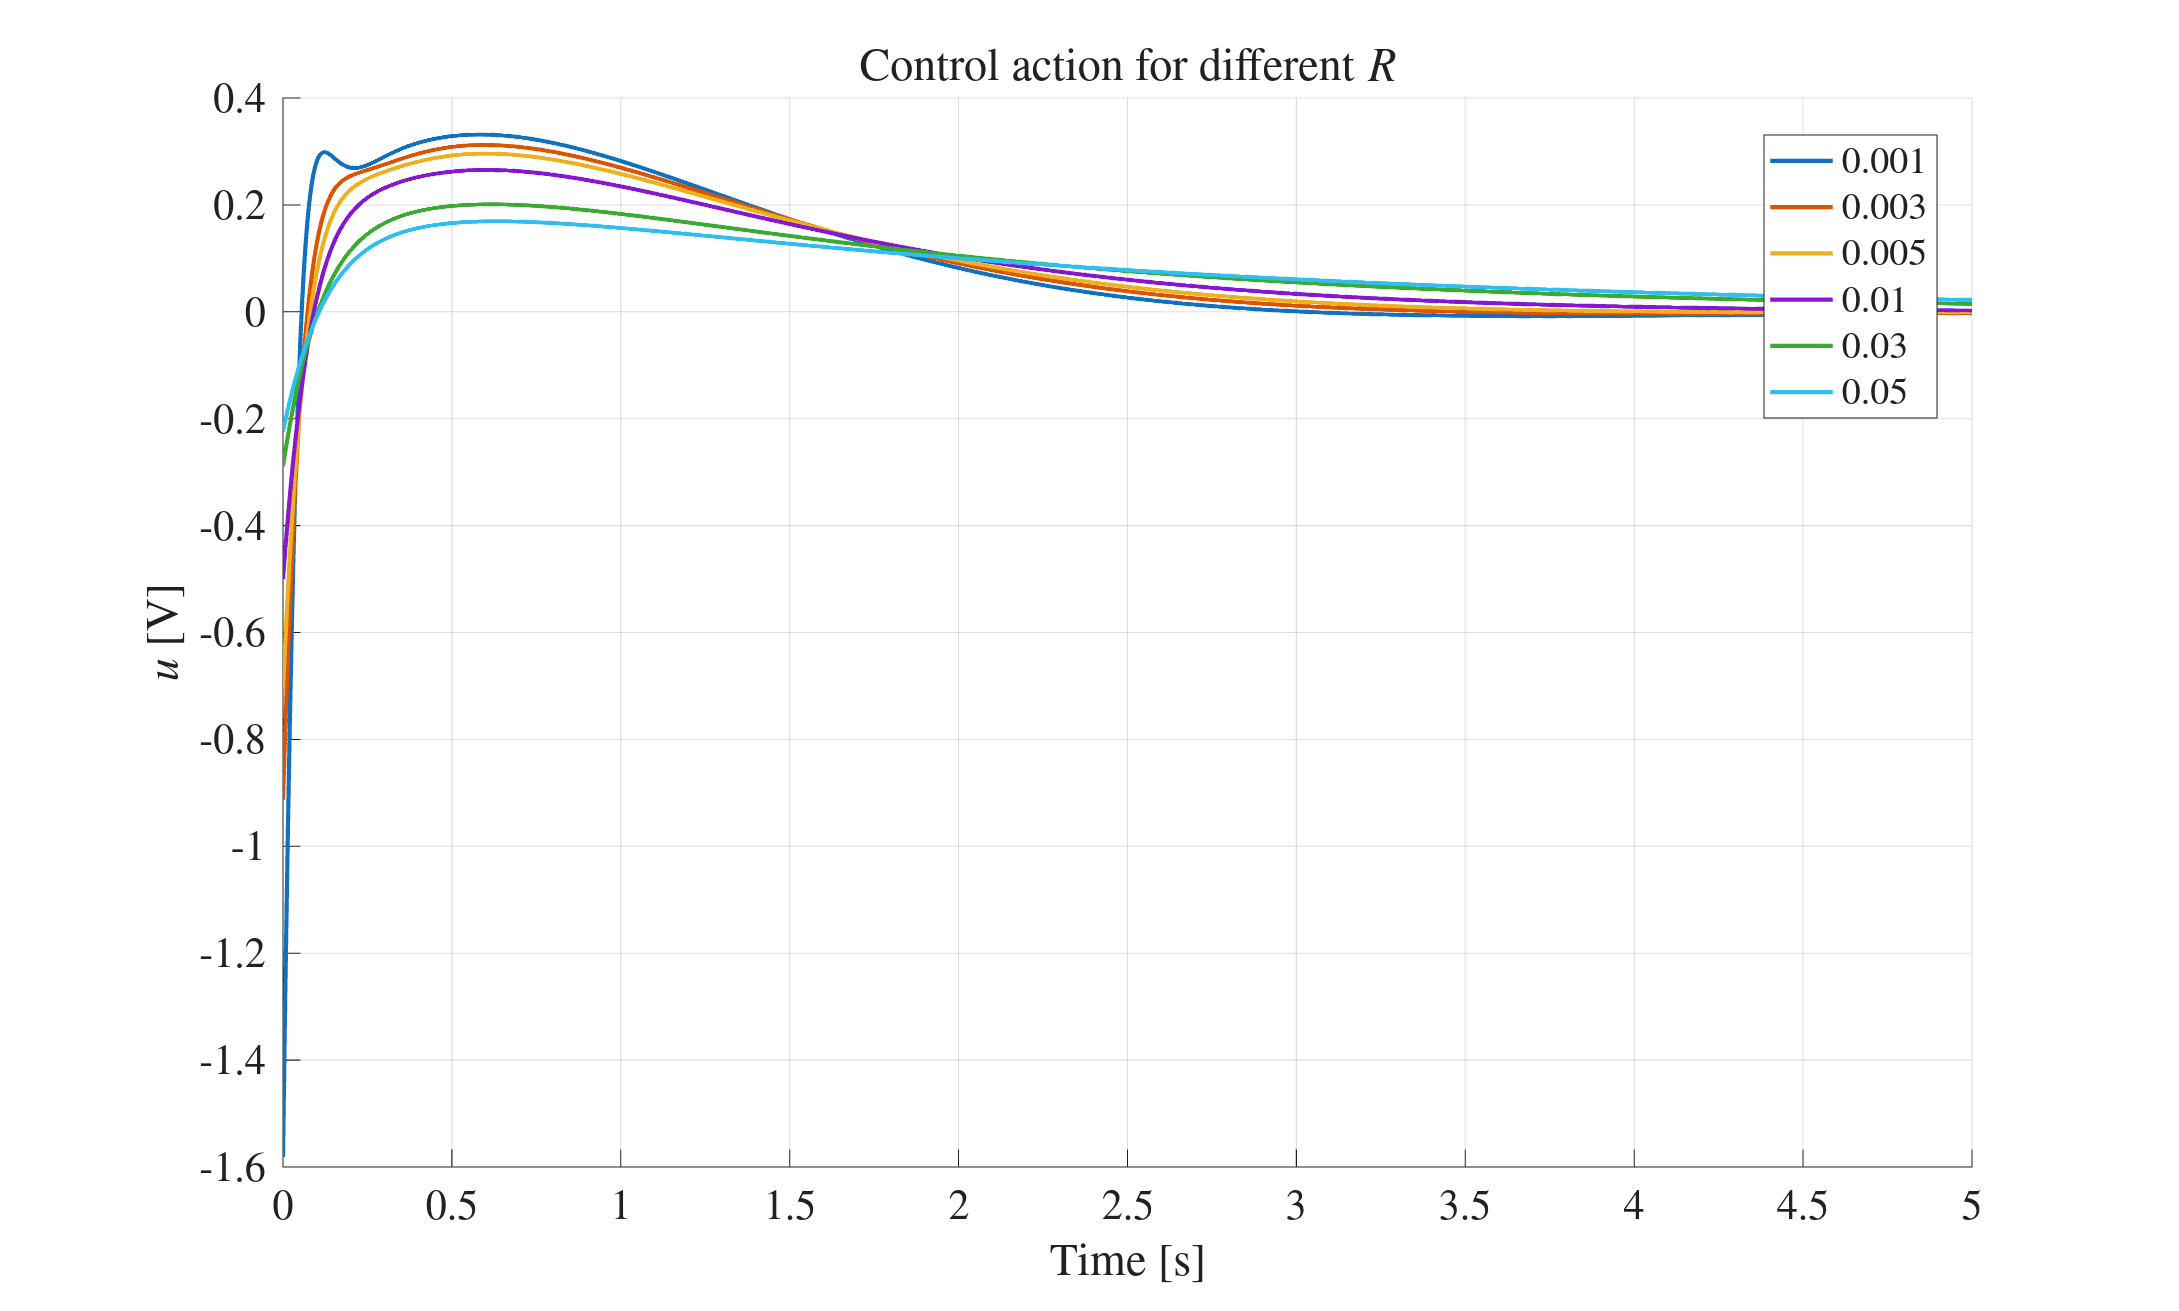
\includegraphics[width=\linewidth]{figures/r_voltage.png}
    \caption{Control action evolution.}
  \end{subfigure}
  \begin{subfigure}{0.45\textwidth}
    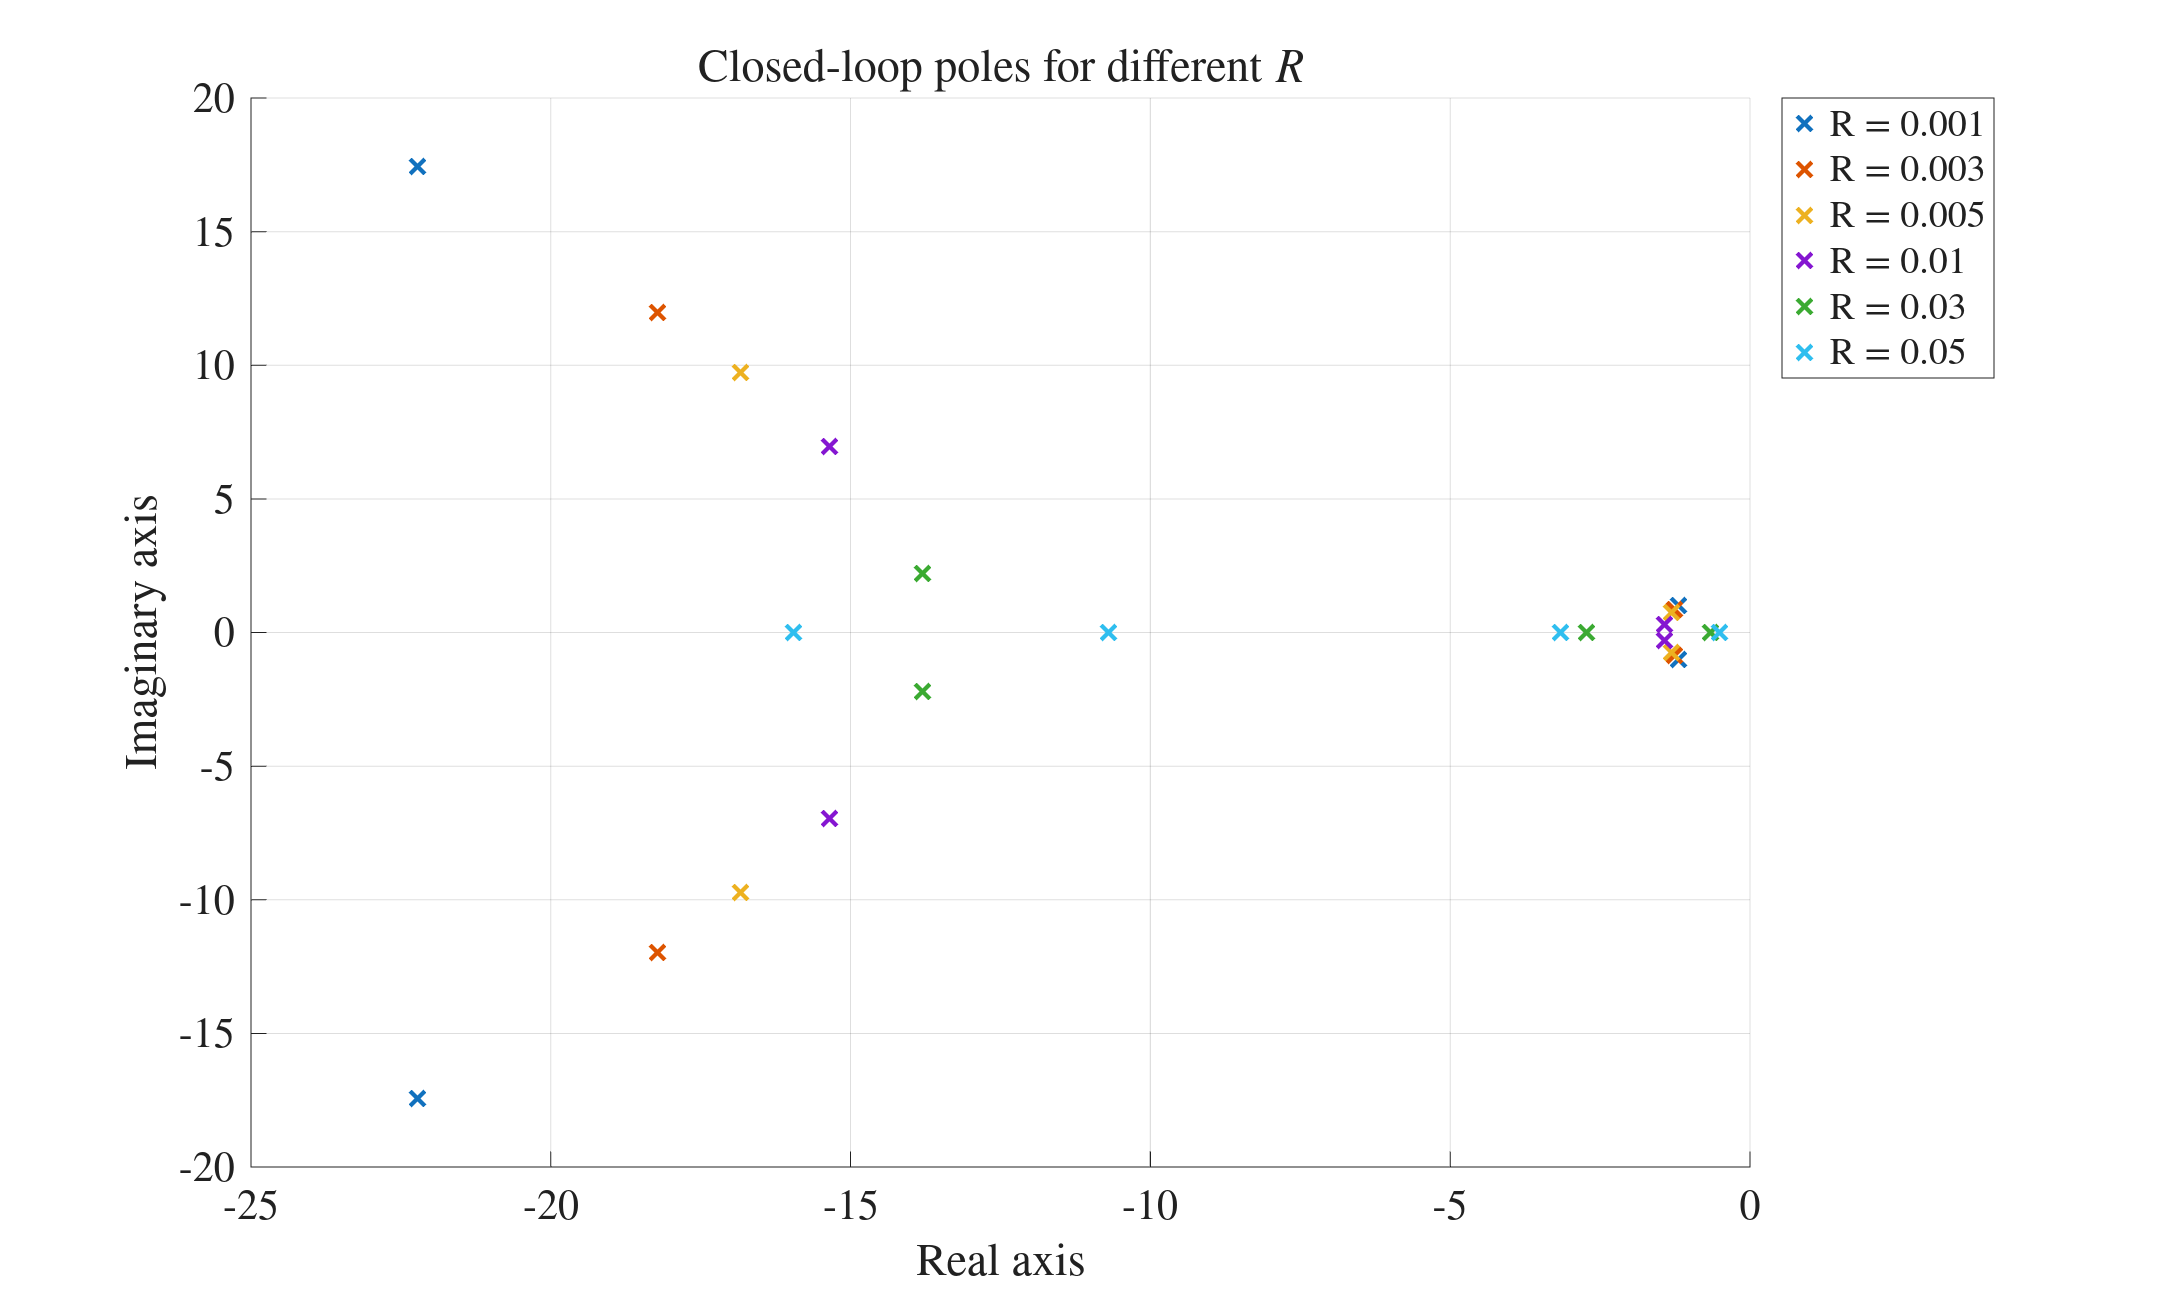
\includegraphics[width=\linewidth]{figures/r_poles.png}
    \caption{Poles of the system.}
  \end{subfigure}
  \caption{Simulation results for different values of $R$.}
  \label{fig:r}
\end{figure} 

\FloatBarrier

\subsection{Setpoint Change on a Chosen Pair $Q$ and $R$}

In this section we try and find a good pair, $Q$ and $R$, by adjusting the values. A good value is one that provides a satisfactory behaviour according to the control objectives. The system is validated by observing the system's response to a set-point change of 10 cm. We start from the $Q_{\text{base}}$ and $R_{\text{base}}$ and perform updates. At each update, we observe the evolution of the states and the control action, and we check if the behaviour is satisfactory. If the systen is not satisfactory, we perform another update through the intuition built in the previous section and continue this process until we find a good pair, $Q$ and $R$, that satisfy the control goals. Table \ref{tab:tuning_data} provides some data on the set-point behaviour of the systems at each update.\\
\\
\begin{enumerate}
  \item Base: Figure \ref{fig:step_base} shows the response of the system to a set-point change of 10 cm for $Q_{\text{base}}$ and $R_{\text{base}}$. The settling time of $x$ is not satisfactory. So, we increase $Q_{1,1}$.
  \begin{figure}[htbp]
  \centering
  \begin{subfigure}{0.45\textwidth}
    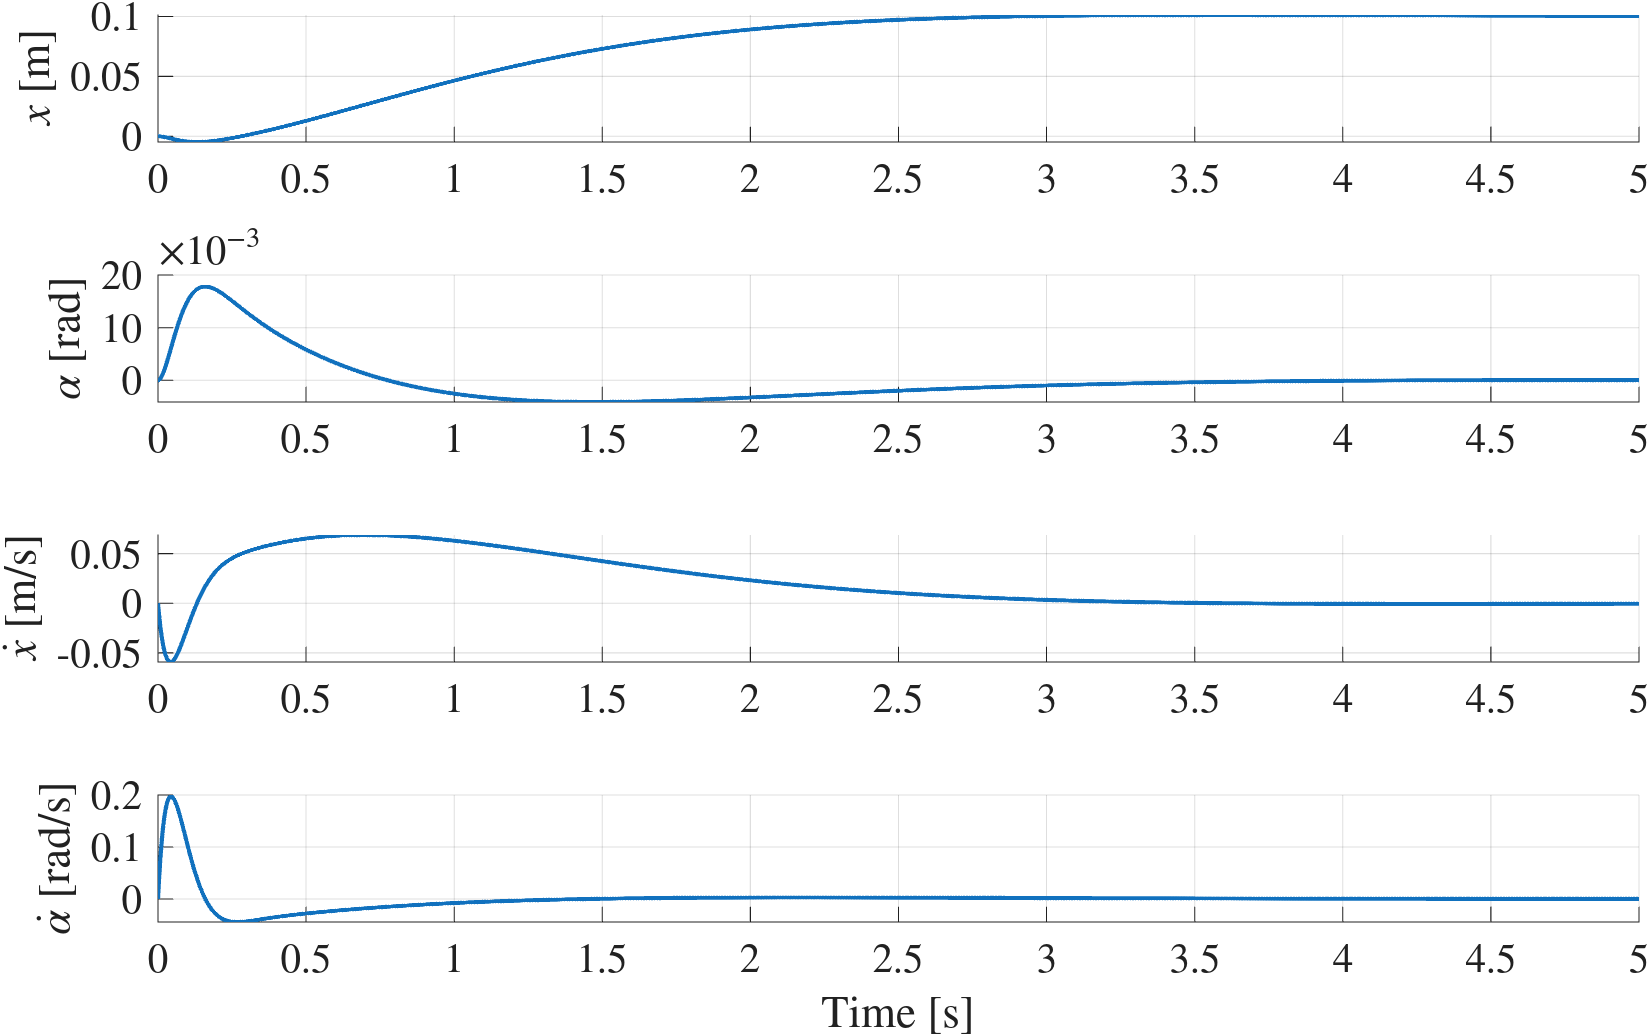
\includegraphics[width=\linewidth]{figures/step_states_base.png}
    \caption{States evolution.}
  \end{subfigure}
  \begin{subfigure}{0.45\textwidth}
    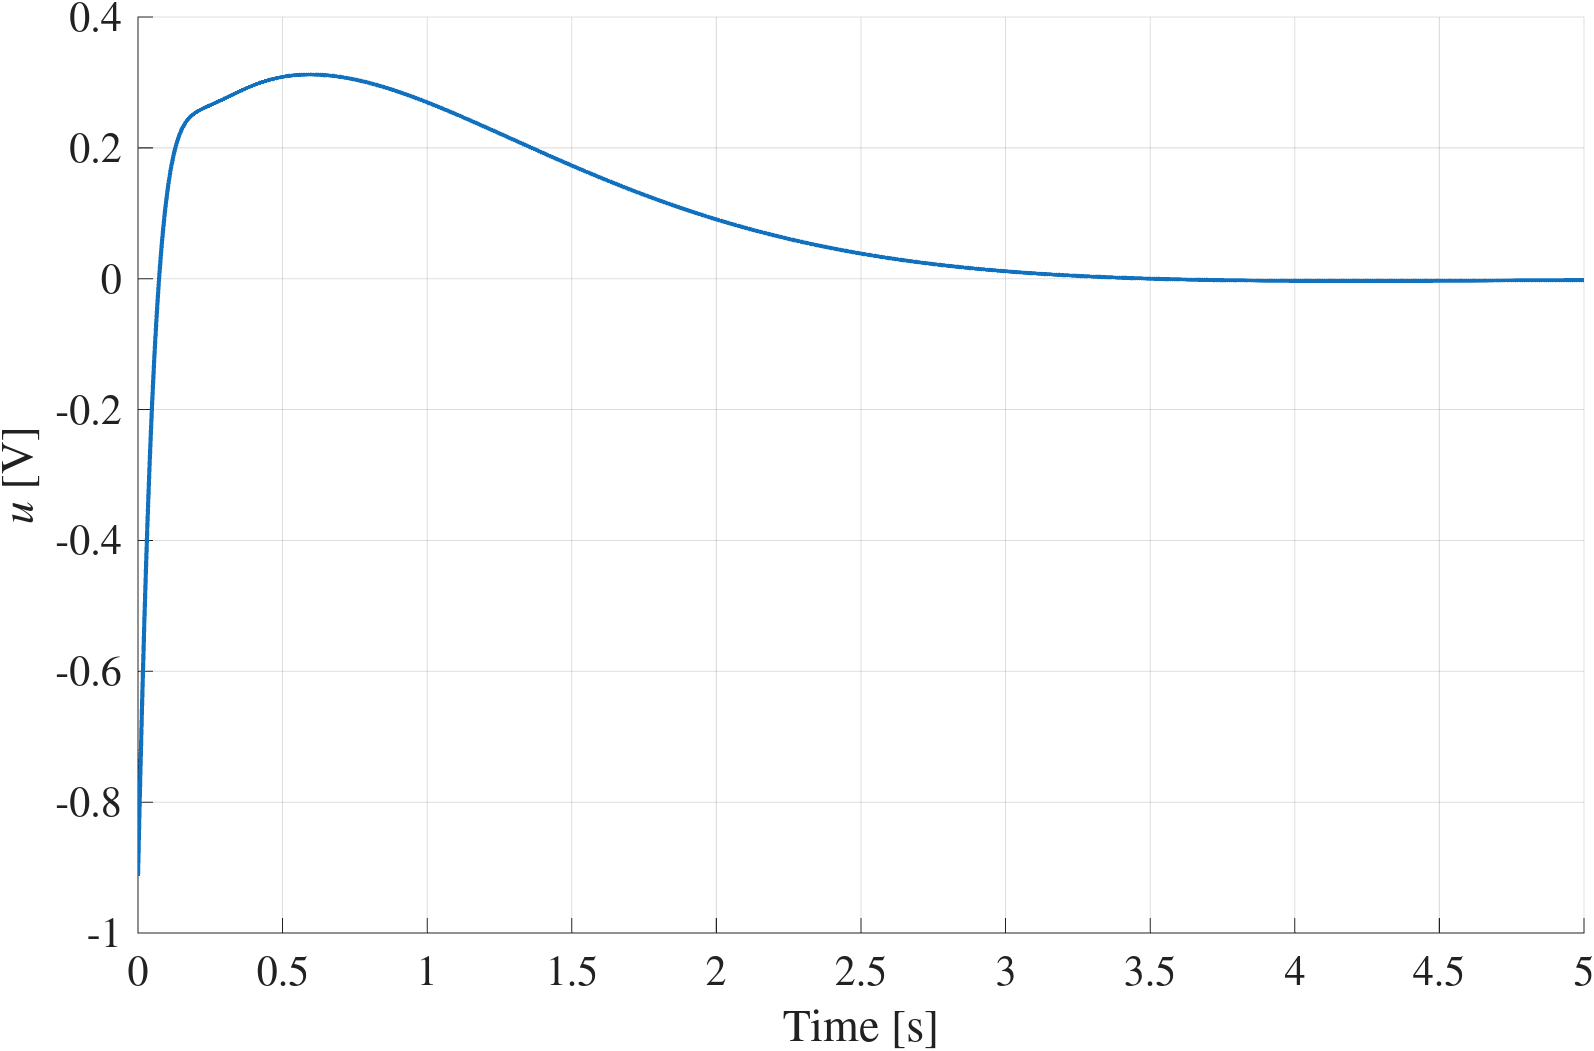
\includegraphics[width=\linewidth]{figures/step_volt_base.png}
    \caption{Control action evolution.}
  \end{subfigure}
  \caption{Response of the system to setpoint change for the closed loop system with a controller computed by LQR with $Q_{\text{base}}$ and $R_{\text{base}}$.}
  \label{fig:step_base}
\end{figure} 

  \item $Q_{1,1}$ = 5: Figure \ref{fig:step_1} shows the response of the system to a set-point change of 10 cm for $Q_{1,1} = 5$. The settling time of $x$  is lower. However, the maximal angle has significantly increased and the control action is much larger in magnitude. We first fix the angle by increasing $Q_{2,2}$ to  . This will reduce the peak in the angle and will also reduce the peak in the control action. However, the main concern of the control action is that it starts at a very low value. This can only be increased through a different $R$ value.
  
  \begin{figure}[htbp]
  \centering
  \begin{subfigure}{0.45\textwidth}
    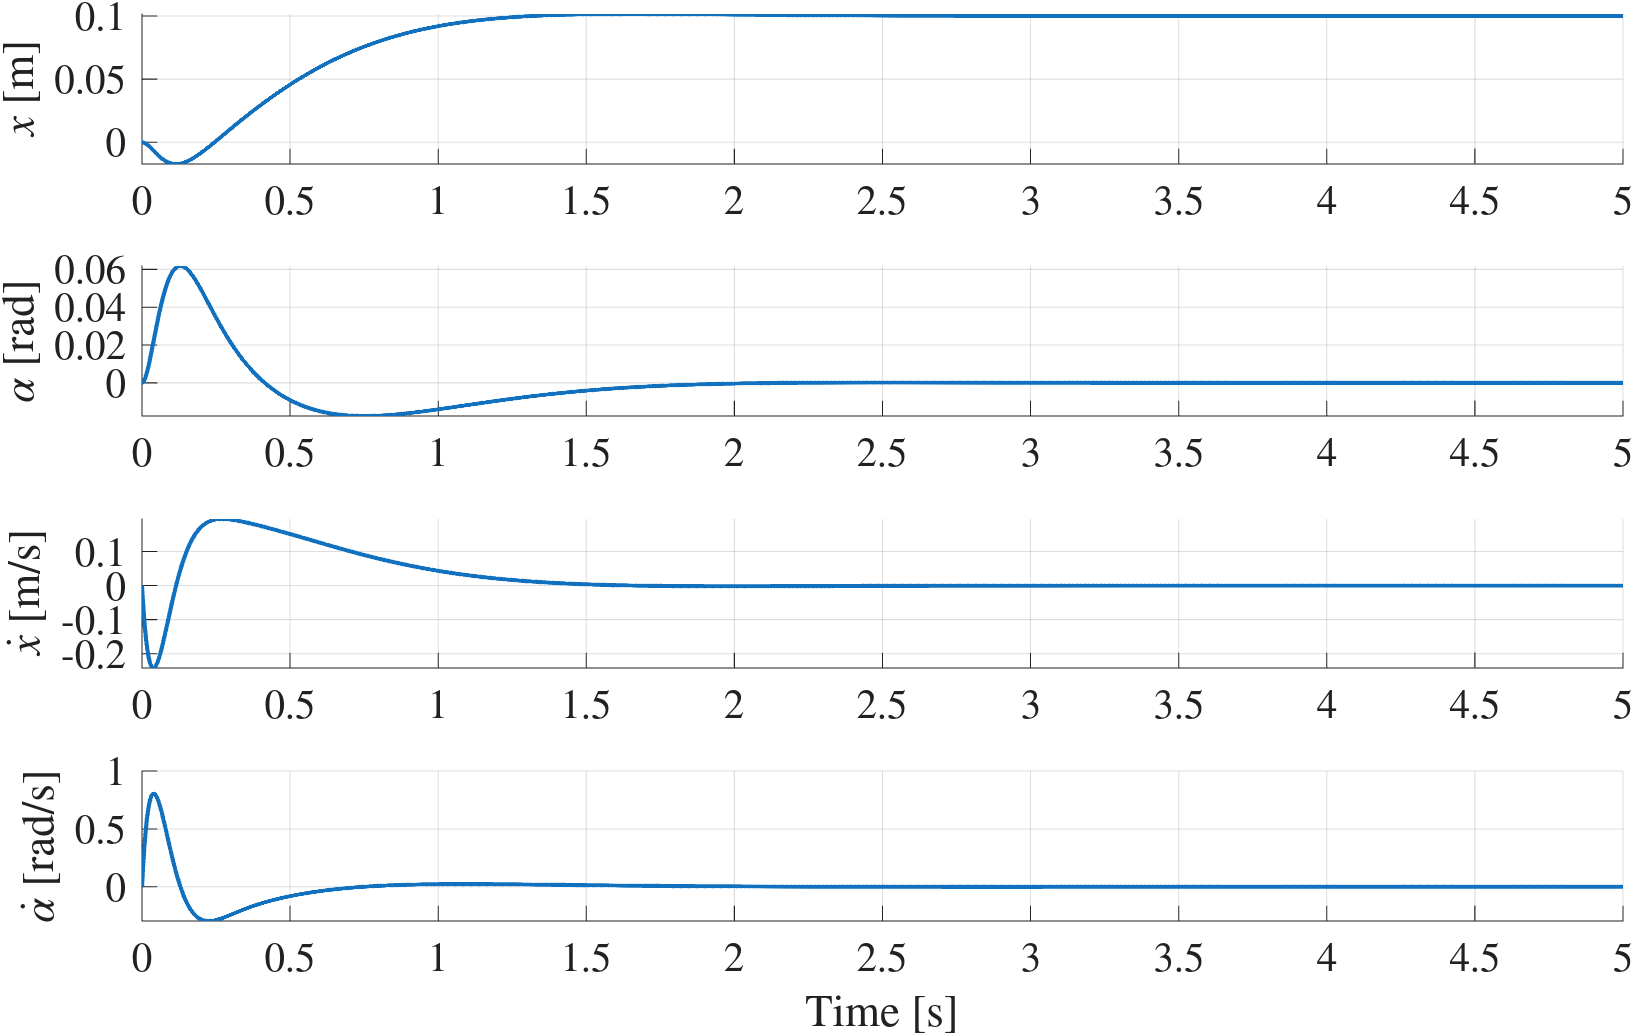
\includegraphics[width=\linewidth]{figures/step_states_1.png}
    \caption{States evolution.}
  \end{subfigure}
  \begin{subfigure}{0.45\textwidth}
    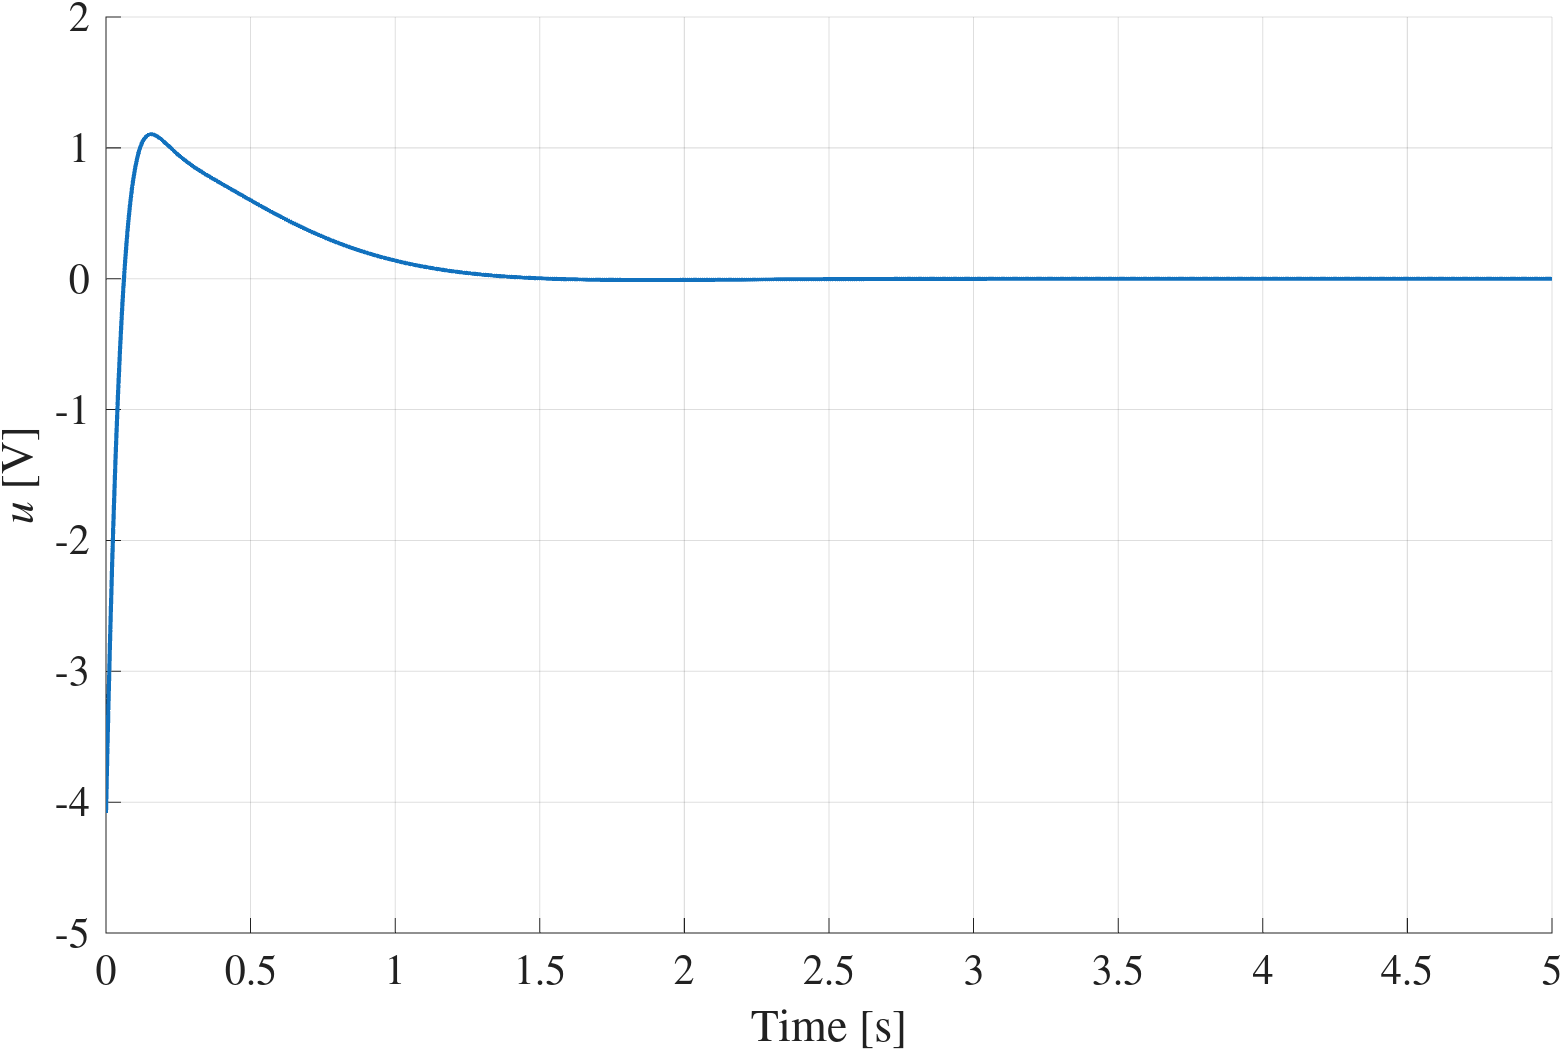
\includegraphics[width=\linewidth]{figures/step_volt_1.png}
    \caption{Control action evolution.}
  \end{subfigure}
  \caption{Response of the system to setpoint change for the closed loop system with a controller computed by LQR with $Q_{1,1} = 5$ and the rest of the values equal to the base values.}
  \label{fig:step_1}
\end{figure} 

  \item $Q_{2,2}$ = 8: Figure \ref{fig:step_2} shows the response of the system to a set-point change for $Q_{2,2} = 8$ and $Q_{1,1} = 5$. The peak of the angle is reduced and the peak of the control action is smaller in magnitude. The settling time of $x$ did increase and the control action starts from the same value as the previous change. This is all observed from the figures and table \ref{tab:tuning_data} and is all as expected. The next step is to increase $R$ to increase the starting value of the control action and to reduce the peaks of the control action. The settling time of $x$ will increase as a result, but this is worth it to avoid saturation. For larger set-point changes, this will definitely be the case with the current controller. For smaller set-point changes, the current controller might be sufficient and increasing $R$ might not be necessary.

  \begin{figure}[htbp]
  \centering
  \begin{subfigure}{0.45\textwidth}
    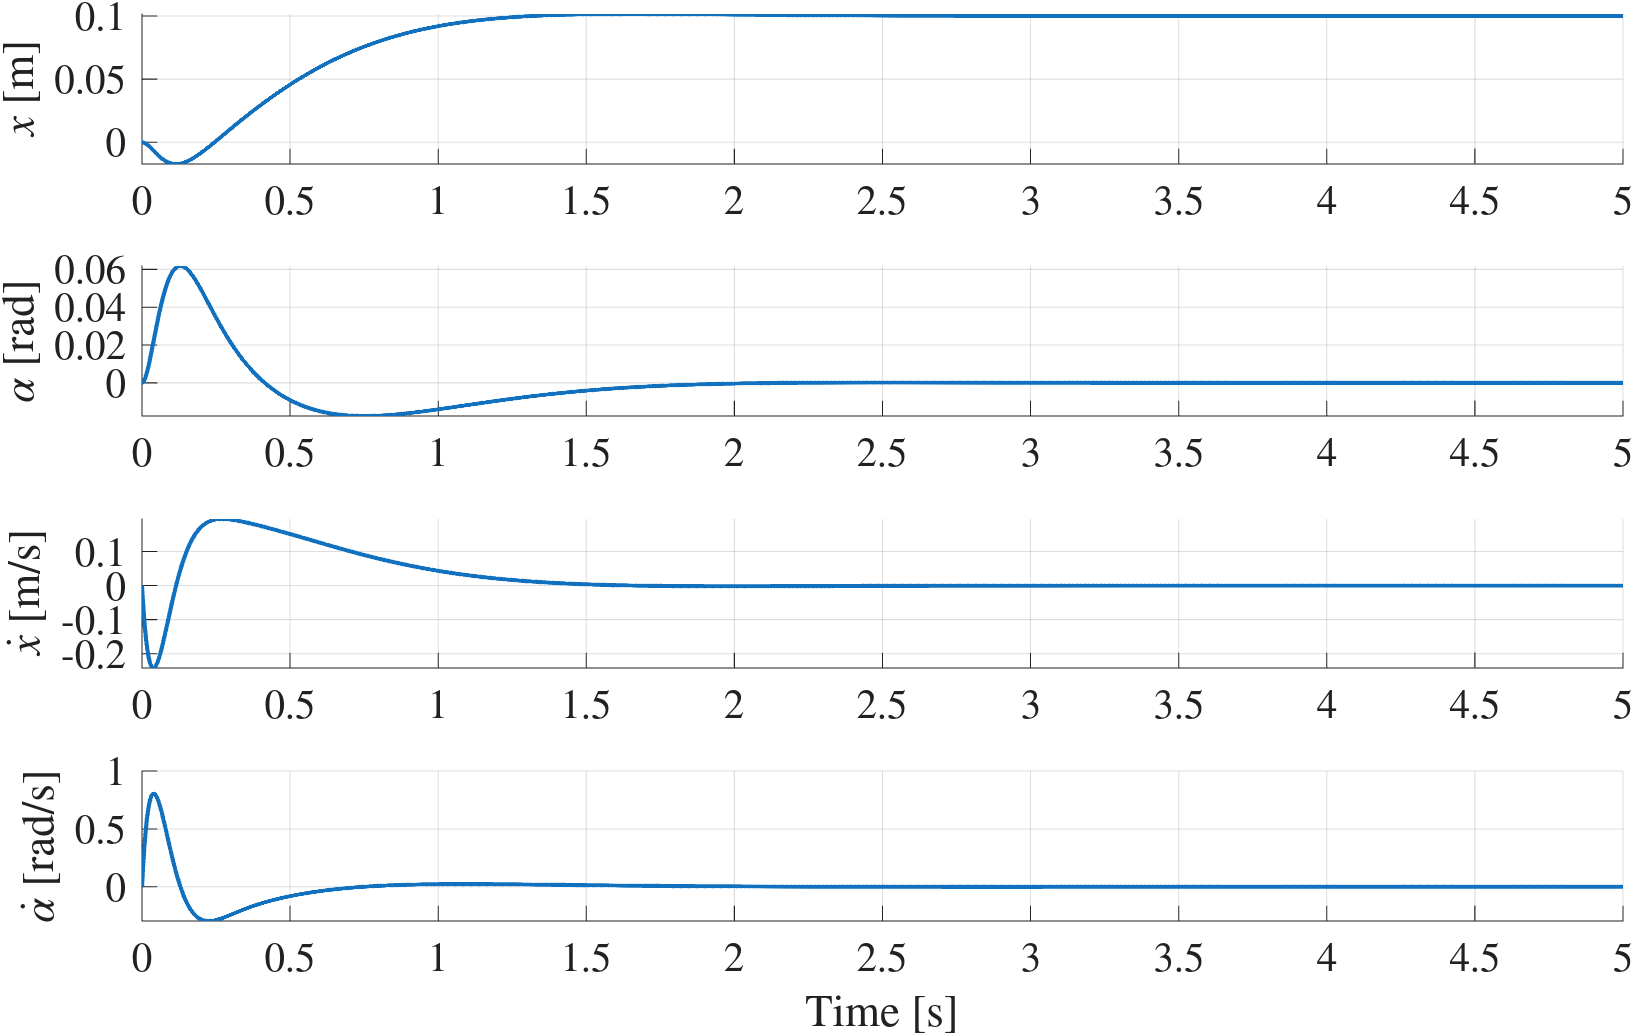
\includegraphics[width=\linewidth]{figures/step_states_2.png}
    \caption{States evolution.}
  \end{subfigure}
  \begin{subfigure}{0.45\textwidth}
    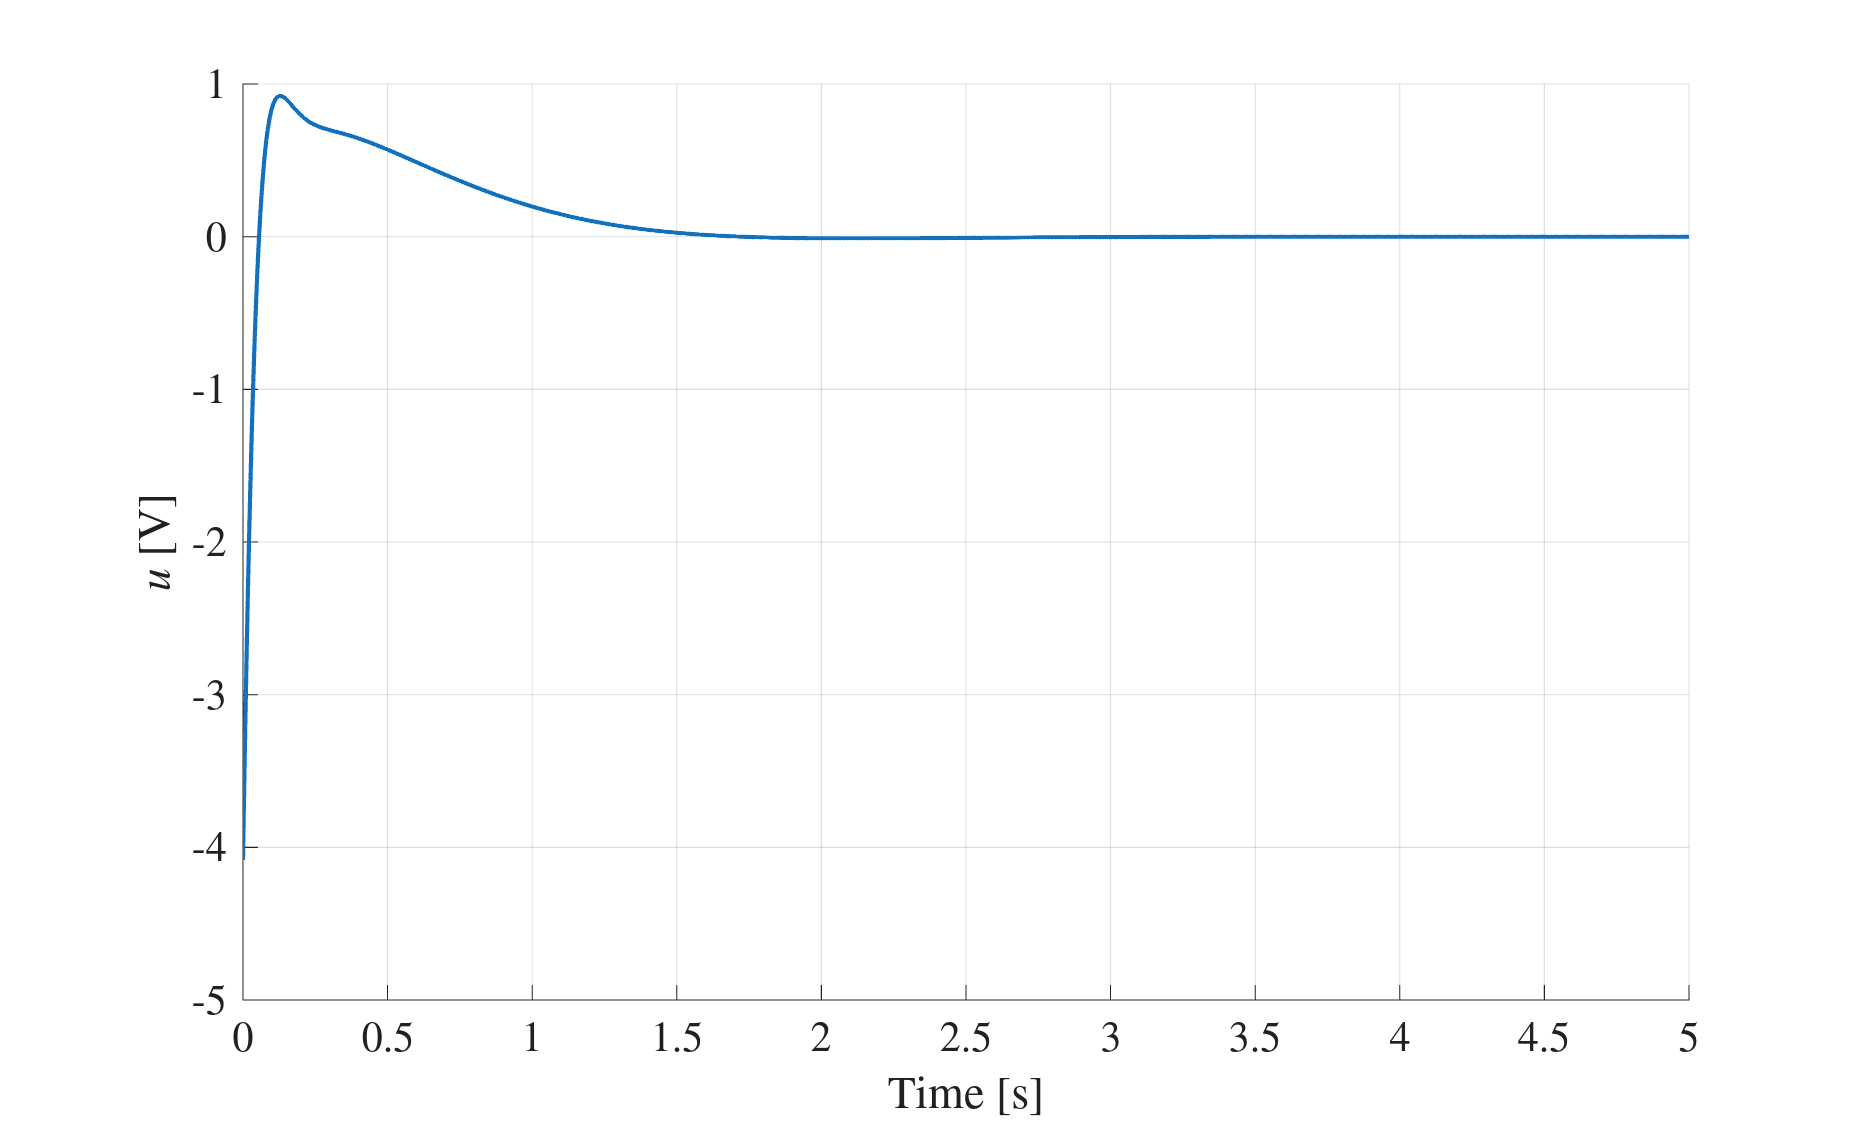
\includegraphics[width=\linewidth]{figures/step_volt_2.png}
    \caption{Control action evolution.}
  \end{subfigure}
  \caption{Response of the system to setpoint change for the closed loop system with a controller computed by LQR with $Q_{1,1} = 5, Q_{2,2} = 8$ and the rest of the values equal to the base values.}
  \label{fig:step_2}
\end{figure} 

  \item $R = 0.03$: Figure \ref{fig:step_3} shows the response of the system to a set-point change for $R = 0.03$, $Q_{1,1} = 5$ and $Q_{2,2} = 8$. The control action starts at a higher value and the peaks of the control action are smaller in magnitude. Although, we expected the settling time of $x$ to increase, it actually decreased. It shows that even though we have a build a certain intuition on how to tune, it still is not a bad idea to have a try and see the results. 
  
  \begin{figure}[htbp]
  \centering
  \begin{subfigure}{0.45\textwidth}
    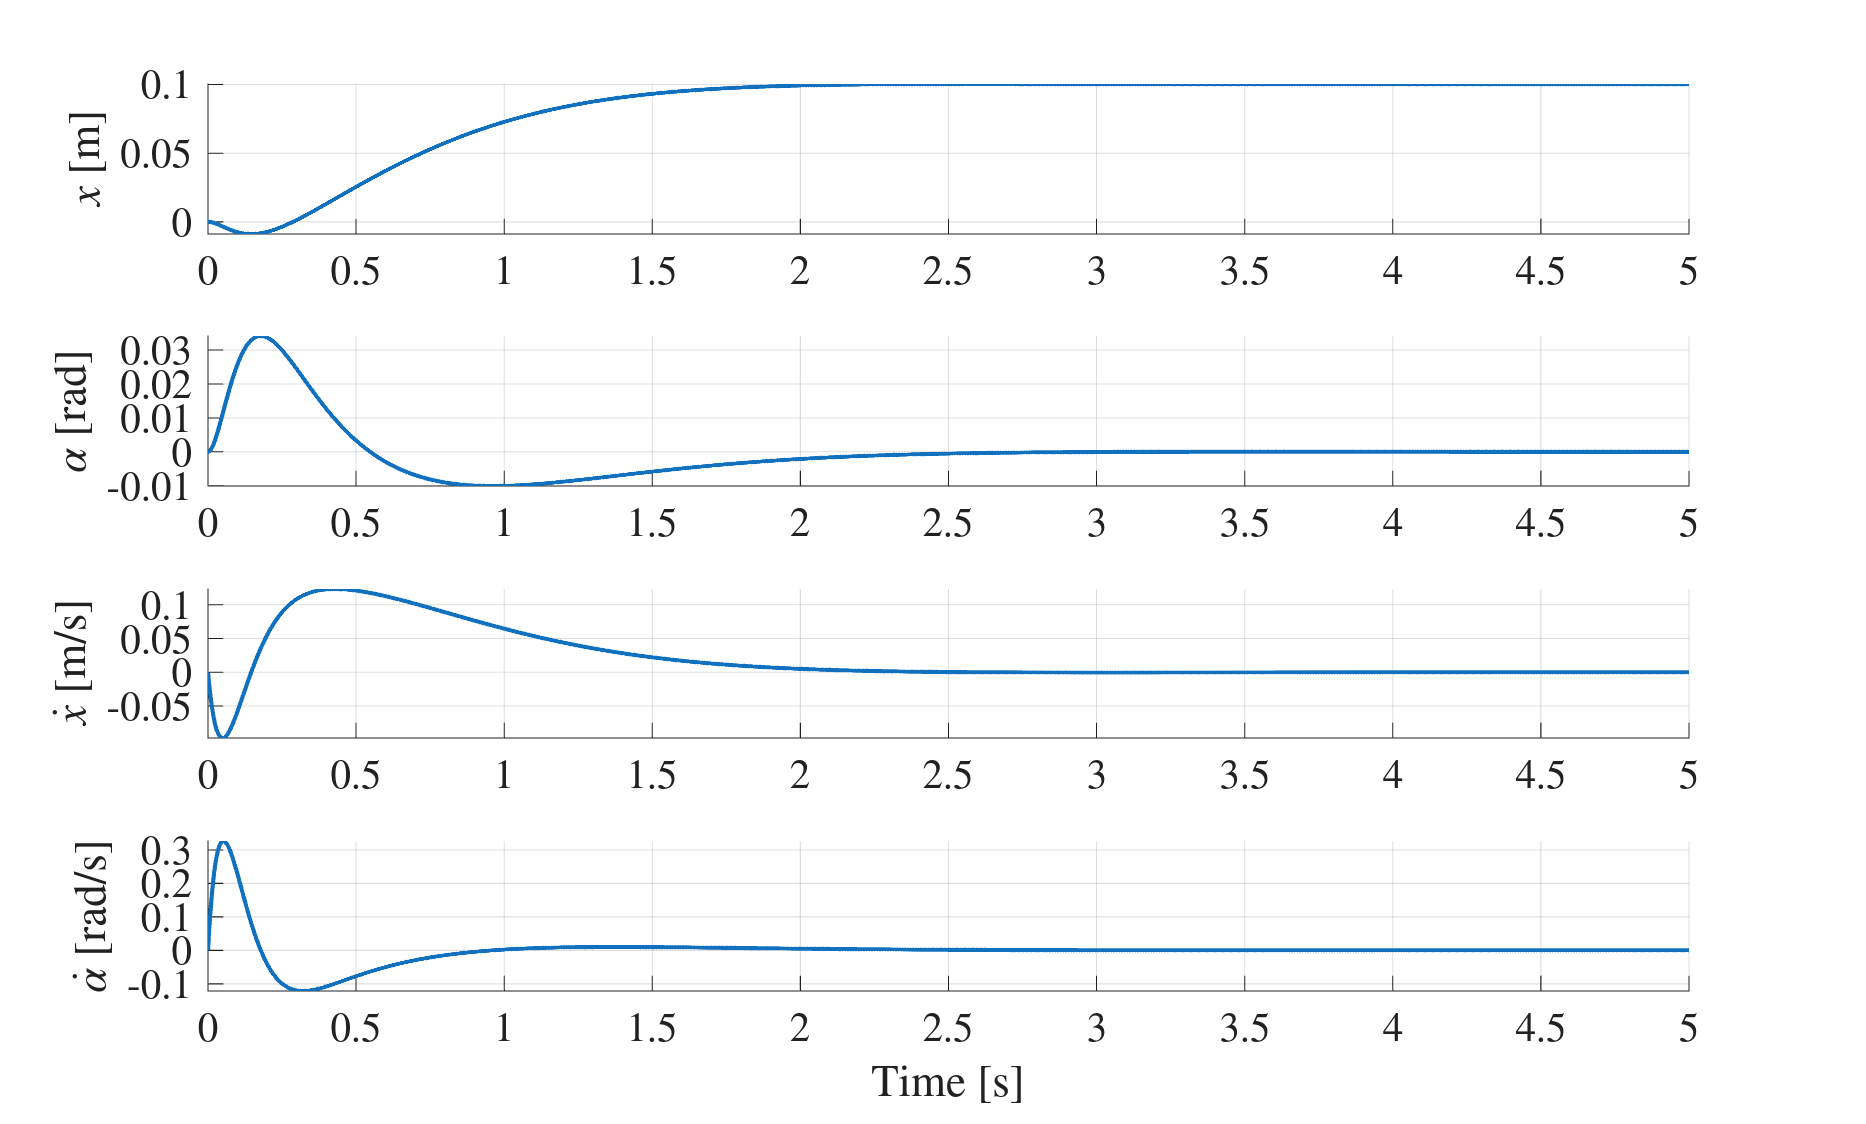
\includegraphics[width=\linewidth]{figures/step_states_3.png}
    \caption{States evolution.}
  \end{subfigure}
  \begin{subfigure}{0.45\textwidth}
    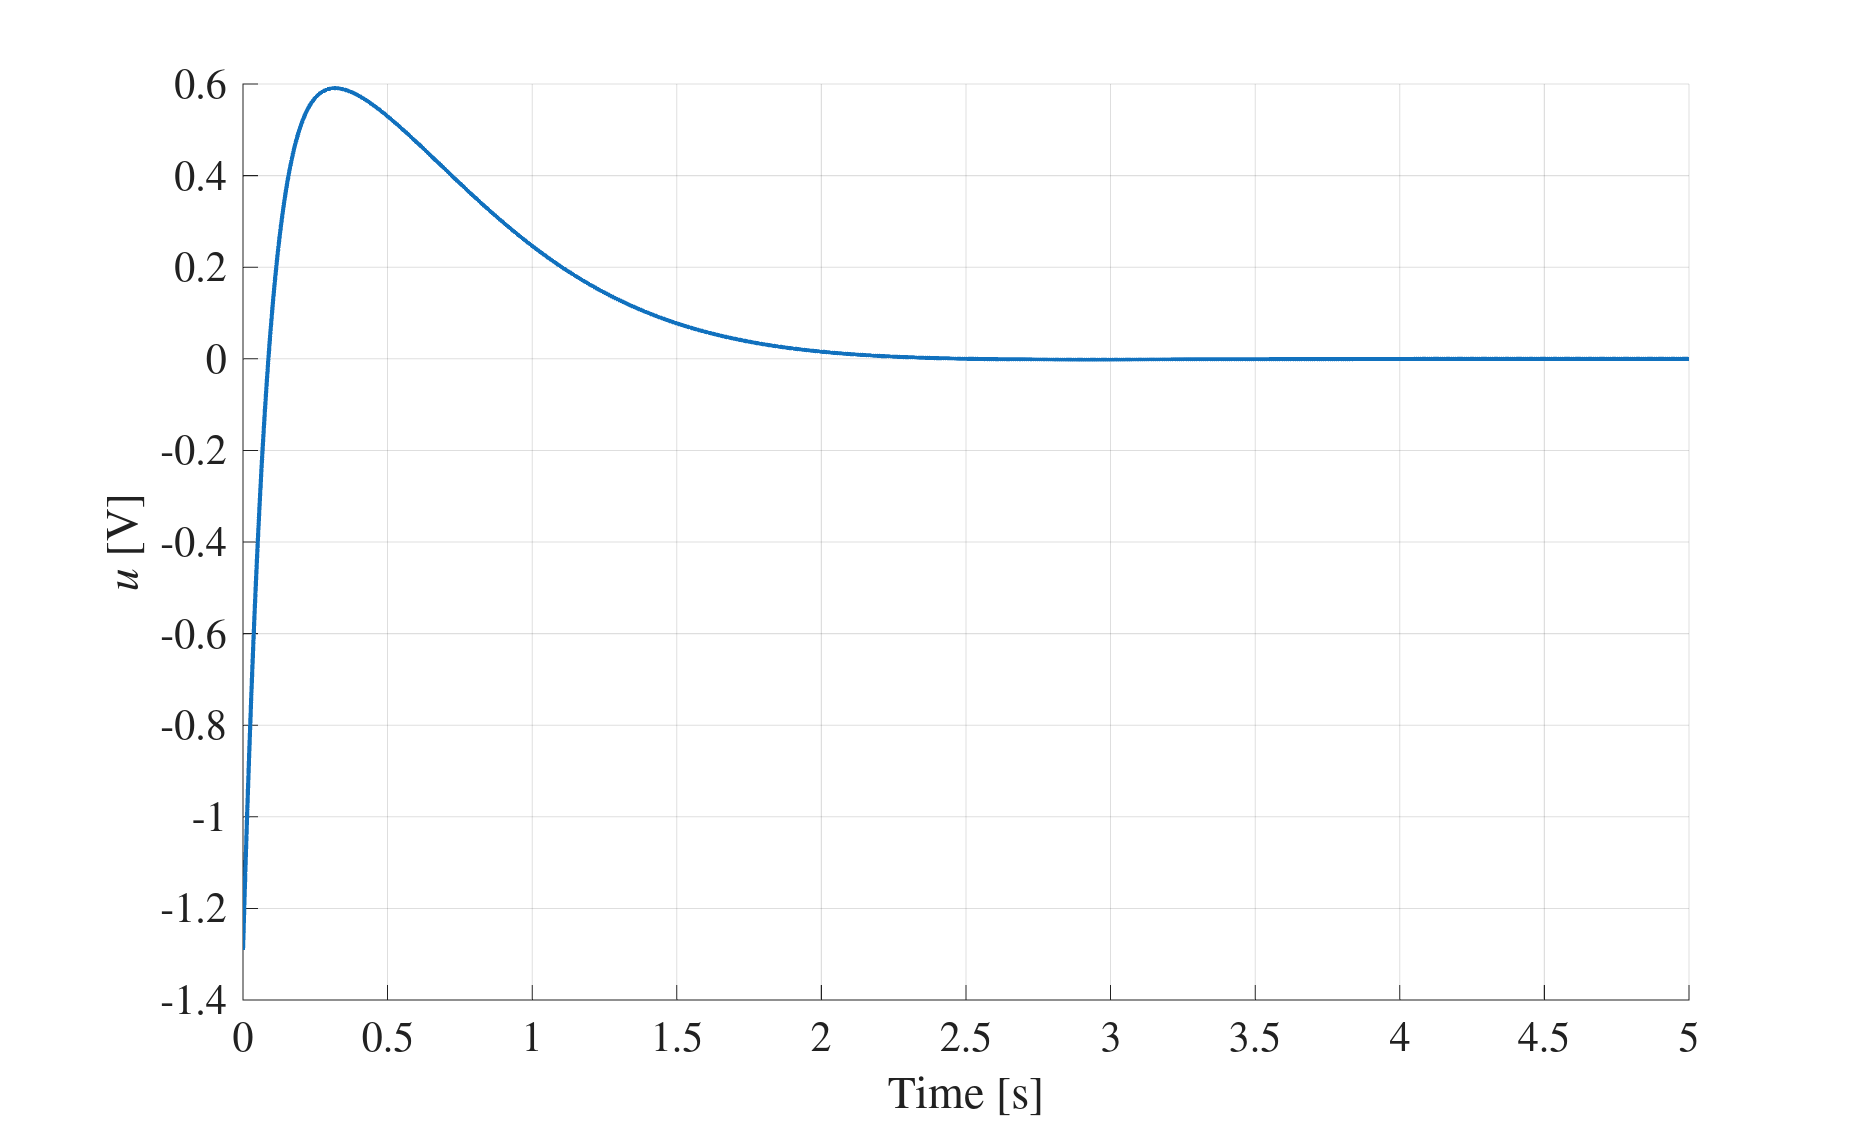
\includegraphics[width=\linewidth]{figures/step_volt_3.png}
    \caption{Control action evolution.}
  \end{subfigure}
  \caption{Response of the system to setpoint change for the closed loop system with a controller computed by LQR with $Q_{1,1} = 5, Q_{2,2} = 8, R = 0.03$ and the rest of the values equal to the base values.}
  \label{fig:step_3}
\end{figure} 

  \item $R = 0.05$: Figure \ref{fig:step_4} shows the response of the system to a set-point change for $R = 0.05$, $Q_{1,1} = 5$ and $Q_{2,2} = 8$. This try was done to see the effect on the behaviour and this time the system behaves as expected. The control action and the angle have become smaller. The settling time of $x$ has increased.
  
  \begin{figure}[htbp]
  \centering
  \begin{subfigure}{0.45\textwidth}
    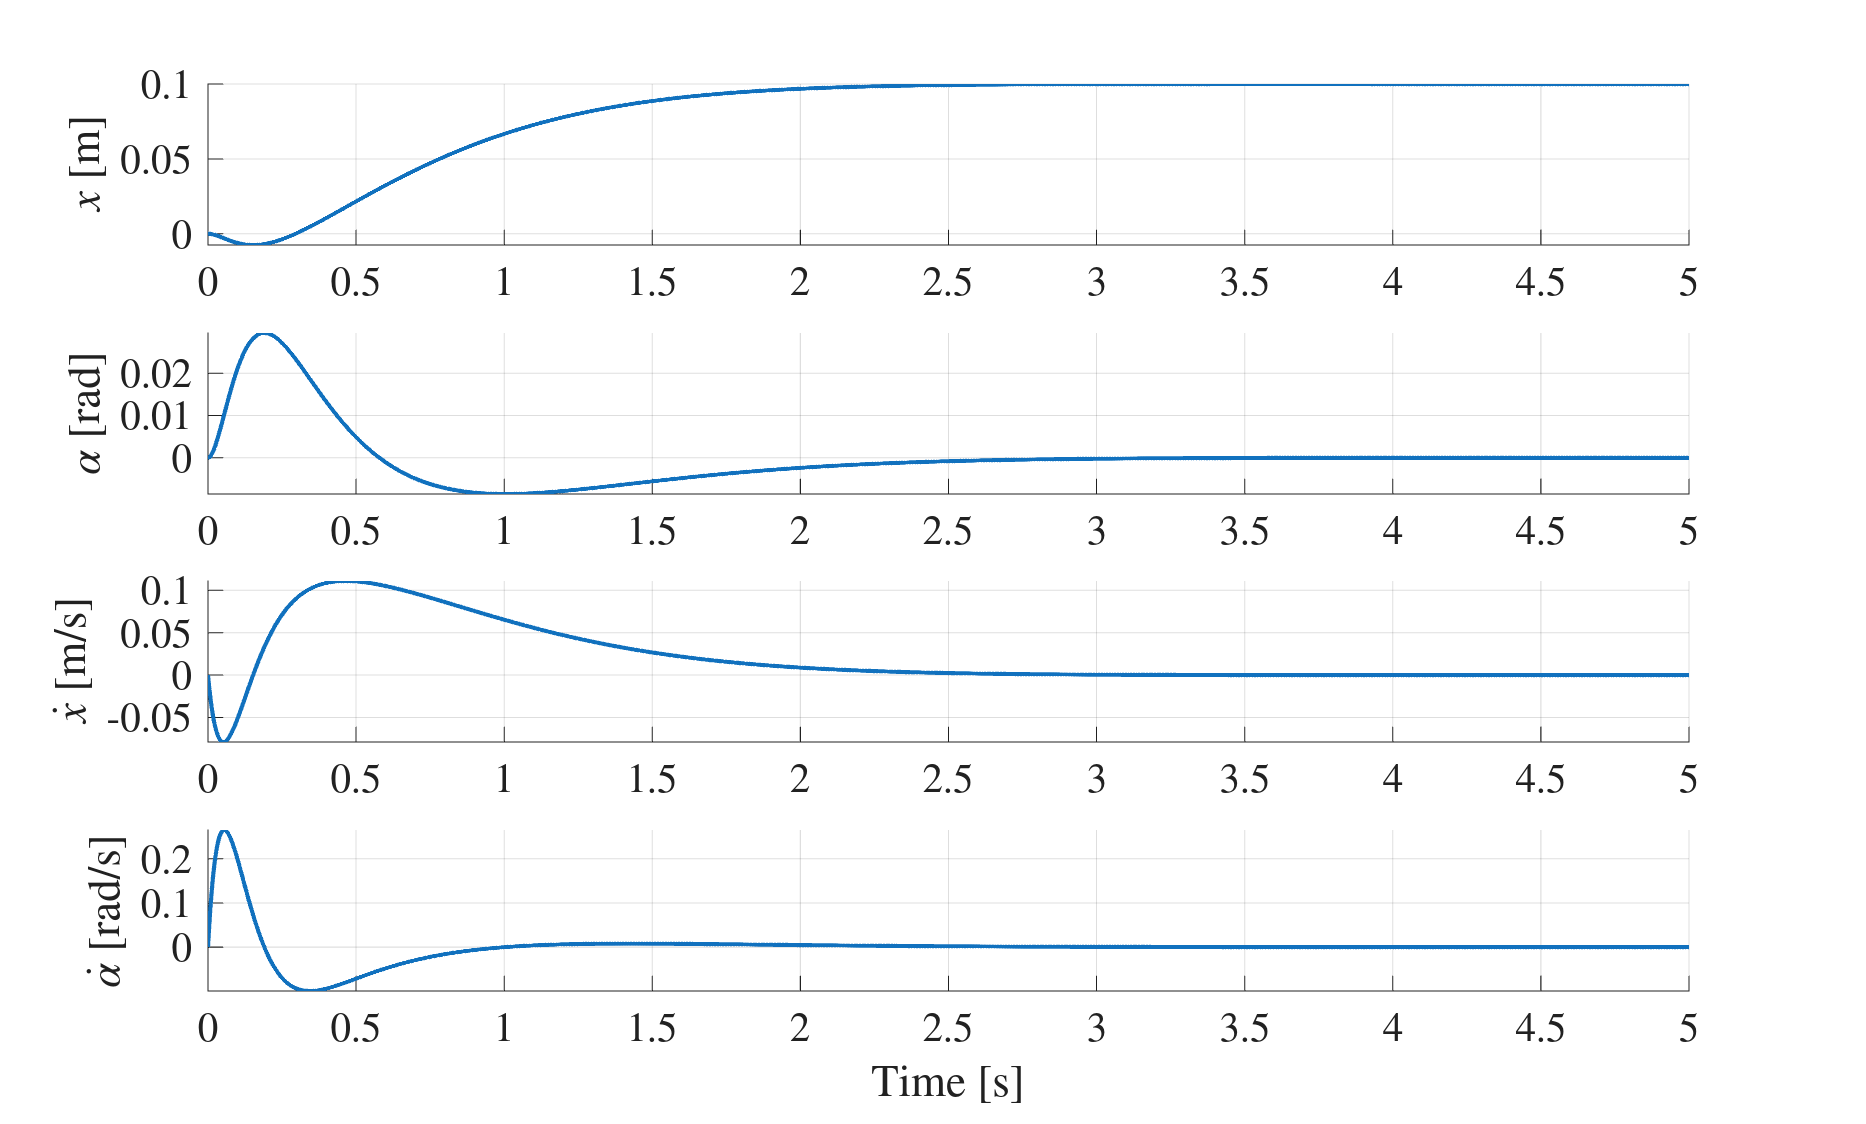
\includegraphics[width=\linewidth]{figures/step_states_4.png}
    \caption{States evolution.}
  \end{subfigure}
  \begin{subfigure}{0.45\textwidth}
    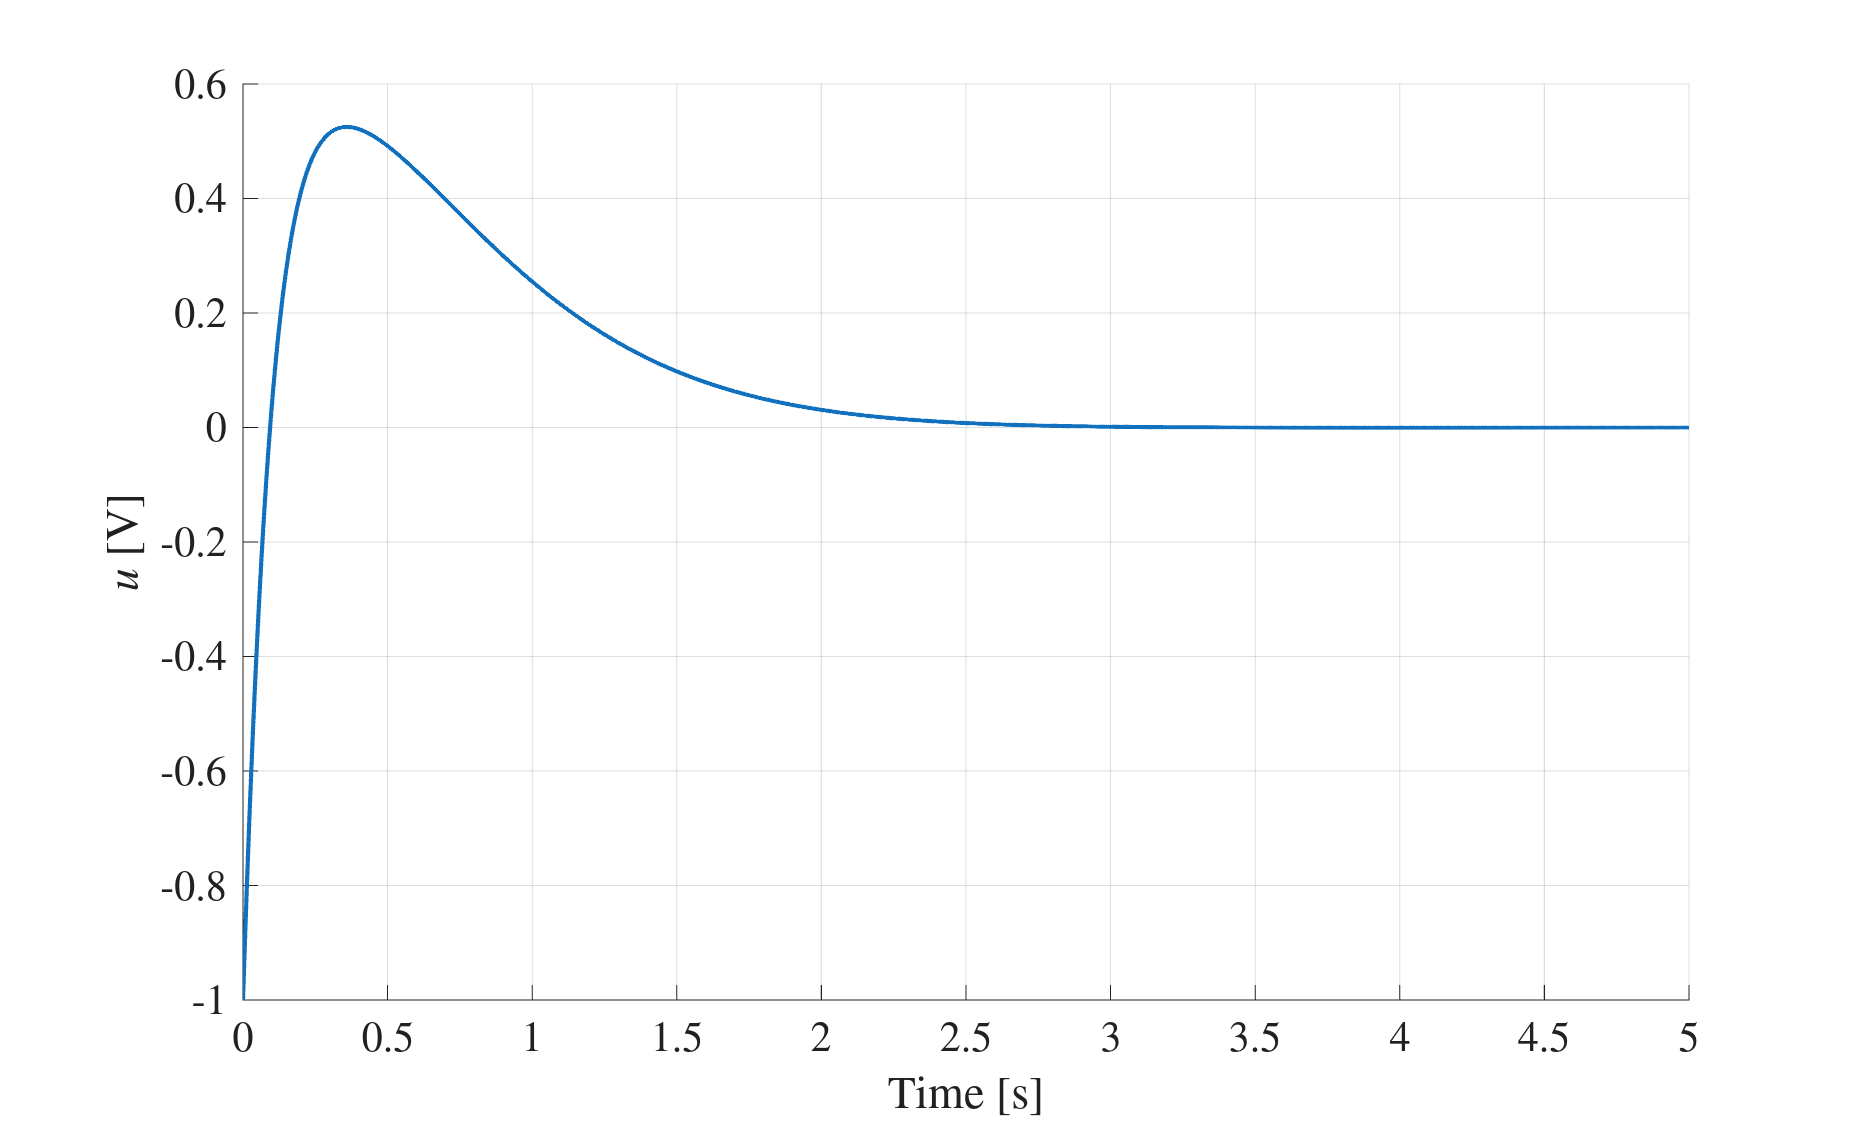
\includegraphics[width=\linewidth]{figures/step_volt_4.png}
    \caption{Control action evolution.}
  \end{subfigure}
  \caption{Response of the system to set-point change for the closed loop system with a controller computed by LQR with $Q_{1,1} = 5, Q_{2,2} = 8, R = 0.05$ and the rest of the values equal to the base values.}
  \label{fig:step_4}
\end{figure} 
\end{enumerate}
\begin{table}[htbp]
\centering
    \begin{tabular}{l|cccc}
        \toprule
          Tuning Step  & $x$ Settling Time & Max $\alpha$ & Time of Max $\alpha$ & Max Absolute Voltage\\
        \midrule
        1. Base & 2.5913  &  0.0178  &  0.1600  &  0.9129 \\
        2. $Q_{1,1} = 5$  &  1.1979  &  0.0618  &  0.1300  &  4.0825 \\
        3. $Q_{2,2} = 8$  &  1.9355  &  0.0520  &  0.1210  &  4.0825 \\
        4. $R = 0.03$  &  1.8226  &  0.0341  &  0.1780  &  1.2910 \\
        5. $R = 0.05$  &  2.1590  &  0.0295  &  0.1900  &  1.0000 \\
        \bottomrule
    \end{tabular}
    \caption{Tuning data for the set-point response of the system.}
    \label{tab:tuning_data}
\end{table}
The values $Q_{3,3}$ and $Q_{4,4}$ are left as zero. Currently, the behaviour of the system satisfies the design requirements. In the next section, a more realistic closed loop model will be presented and the design will be finalized. So, the parameters for the LQR becomes

\begin{equation}
  Q_1 = 
  \begin{bmatrix}
     5 && 0 && 0 && 0 \\
    0 && 8 && 0 && 0 \\
    0 && 0 && 0 && 0 \\
    0 && 0 && 0 && 0 \\
  \end{bmatrix}, \quad
  R_1 = 0.05.
\end{equation}
We chose $R_1 = 0.05$ as the settling time of 2.1590 seconds is for now good enough and will be adjusted in the next sections. More importantly, the angle deviates less and the control action is smaller in magnitude than with $R_1 = 0.03$. 

\section{A More Realistic Closed Loop Model} \label{realistic_closed_loop}

\subsection{Simulink Diagram}

Figure \ref{fig:more_realistic_closed_loop} plots the more realistic closed loop system. Blocks (1), (2), (3), (4) remain the same as in section \ref{closed_loop}. The $C$ matrix in block (1) is no longer the identity matrix, such that the output consists of the measurable states, $x$ and $\alpha$.

\begin{figure}[htbp]
    \centering
    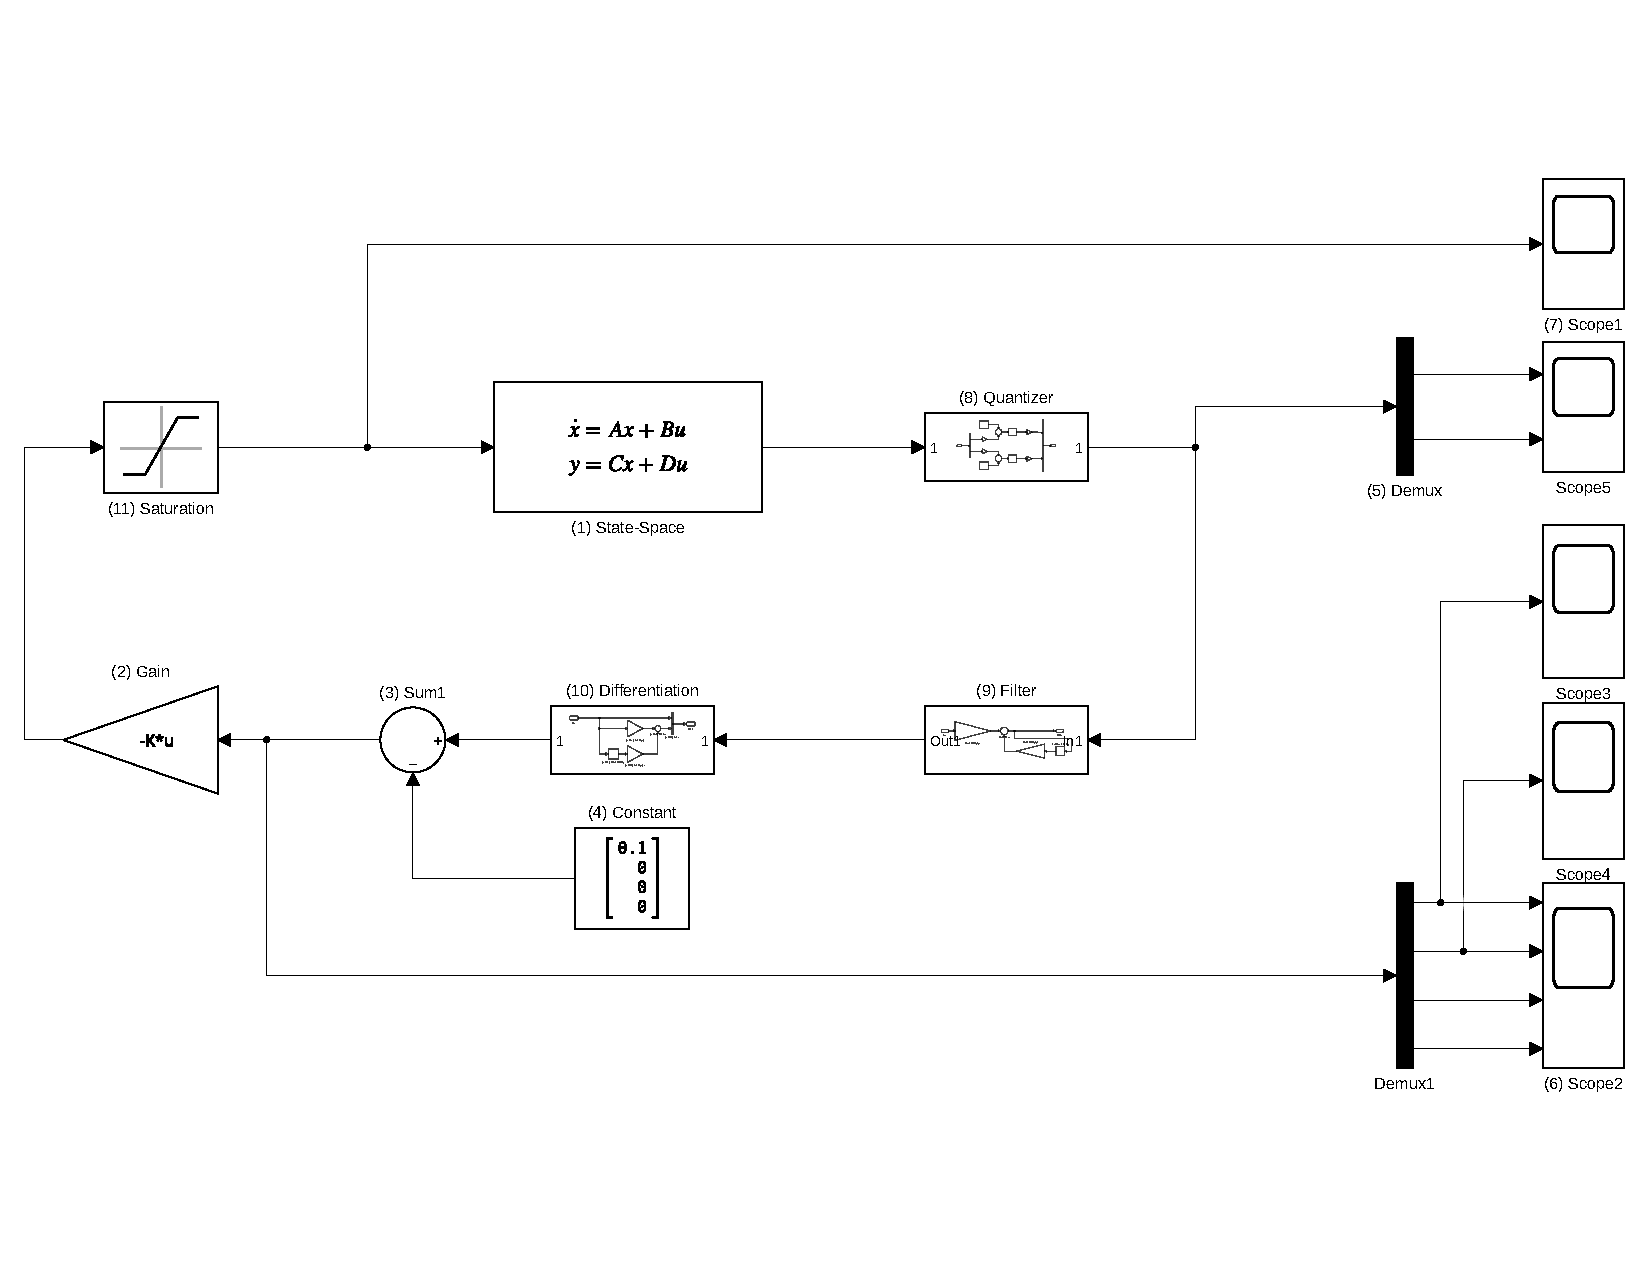
\includegraphics[width=0.8\textwidth]{figures/realistic_closed_loop_system.pdf}
    \caption{The more realistic closed loop simulink diagram.}
    \label{fig:more_realistic_closed_loop}
\end{figure}

The remaining blocks are

\begin{itemize}
  \item \textbf{(8) Quantizer subsystem}: implements the A/D-converter and adds the sensor noise to the measurements. The simulink subsystem is shown in figure \ref{fig:quantizer}. The subsystem first separates the measurements into two separate signals with (8.1) demux block. Each measurement is converted, with (8.2) gain block, to voltage through the respective conversion factors, $F_x$ and $F_\alpha$. The Gaussian random number generators, (8.3) in the simulink diagram, are set to simulate the sensor noise of the measurements. The variation of the noise was estimated by collecting data from the real setup and calculating the variation. Figure \ref{fig:sensor_noise} provides a plot of the collected noise measurements. The simulink noise blocks are both set to zero mean and $10^-9$ variation. Next, the quantizer block (8.4) follows. (8.4) is set to a quantization interval of $\frac{\text{Voltage range}}{2^{\text{resolution bits}}} = \frac{20}{2^{16}} \approx 0.00030518$. Finally, Each signal is returned through the conversion factors to the measurement units with (8.5) and the both signals are combined into a signal vector with the mux block.  
  \item \textbf{(9) Filter subsystem}: implements the low-pass filter of the raw measurements. Figure \ref{fig:filter} shows the simulink diagram of the subsystem. The diagram realises 
  \[ y_n^f = \frac{\omega_c T_s}{1+\omega_cT_s}y_n + \frac{1}{1+\omega_cT_s}y_{n-1}^f.\]
  In the second term, $y_{n-1}^f$ is accomplished through the (9.4) delay block. The two terms are summed with (9.3) and both terms are multiplied with the correct factor through the gain blocks (9.1) and (9.2). The output is forwarded to the next block and also stored in the delay block for the next filter calculation. The delay block is initialised with $\mathbf{0}$.
  \item \textbf{(10) Differentiation subsystem}: calculates the states $\dot{x}$ and $\dot{\alpha}$ using the backward difference equation:
  \[ \dot{y_n} = \frac{y^f_n - y^f_{n-1}}{T_s}.\]
  Figure \ref{fig:differentiation} shows the simulink subsystem diagram. As with the filter subsystem, $y^f_{n-1}$ is obtained with the (10.2) delay block. The mux block (10.5) concatenates all the states into a single vector and the subsystem forwards the result to the control-module. 
  \item \textbf{(11) Saturation}: receives the control action and limits the voltage inputs to the actuator. The saturation limits are set to $-5$ Volts and $+5$ Volts. The signal is forwarded to the state space model in block (1).
\end{itemize}

\begin{figure}[htbp]
    \centering
    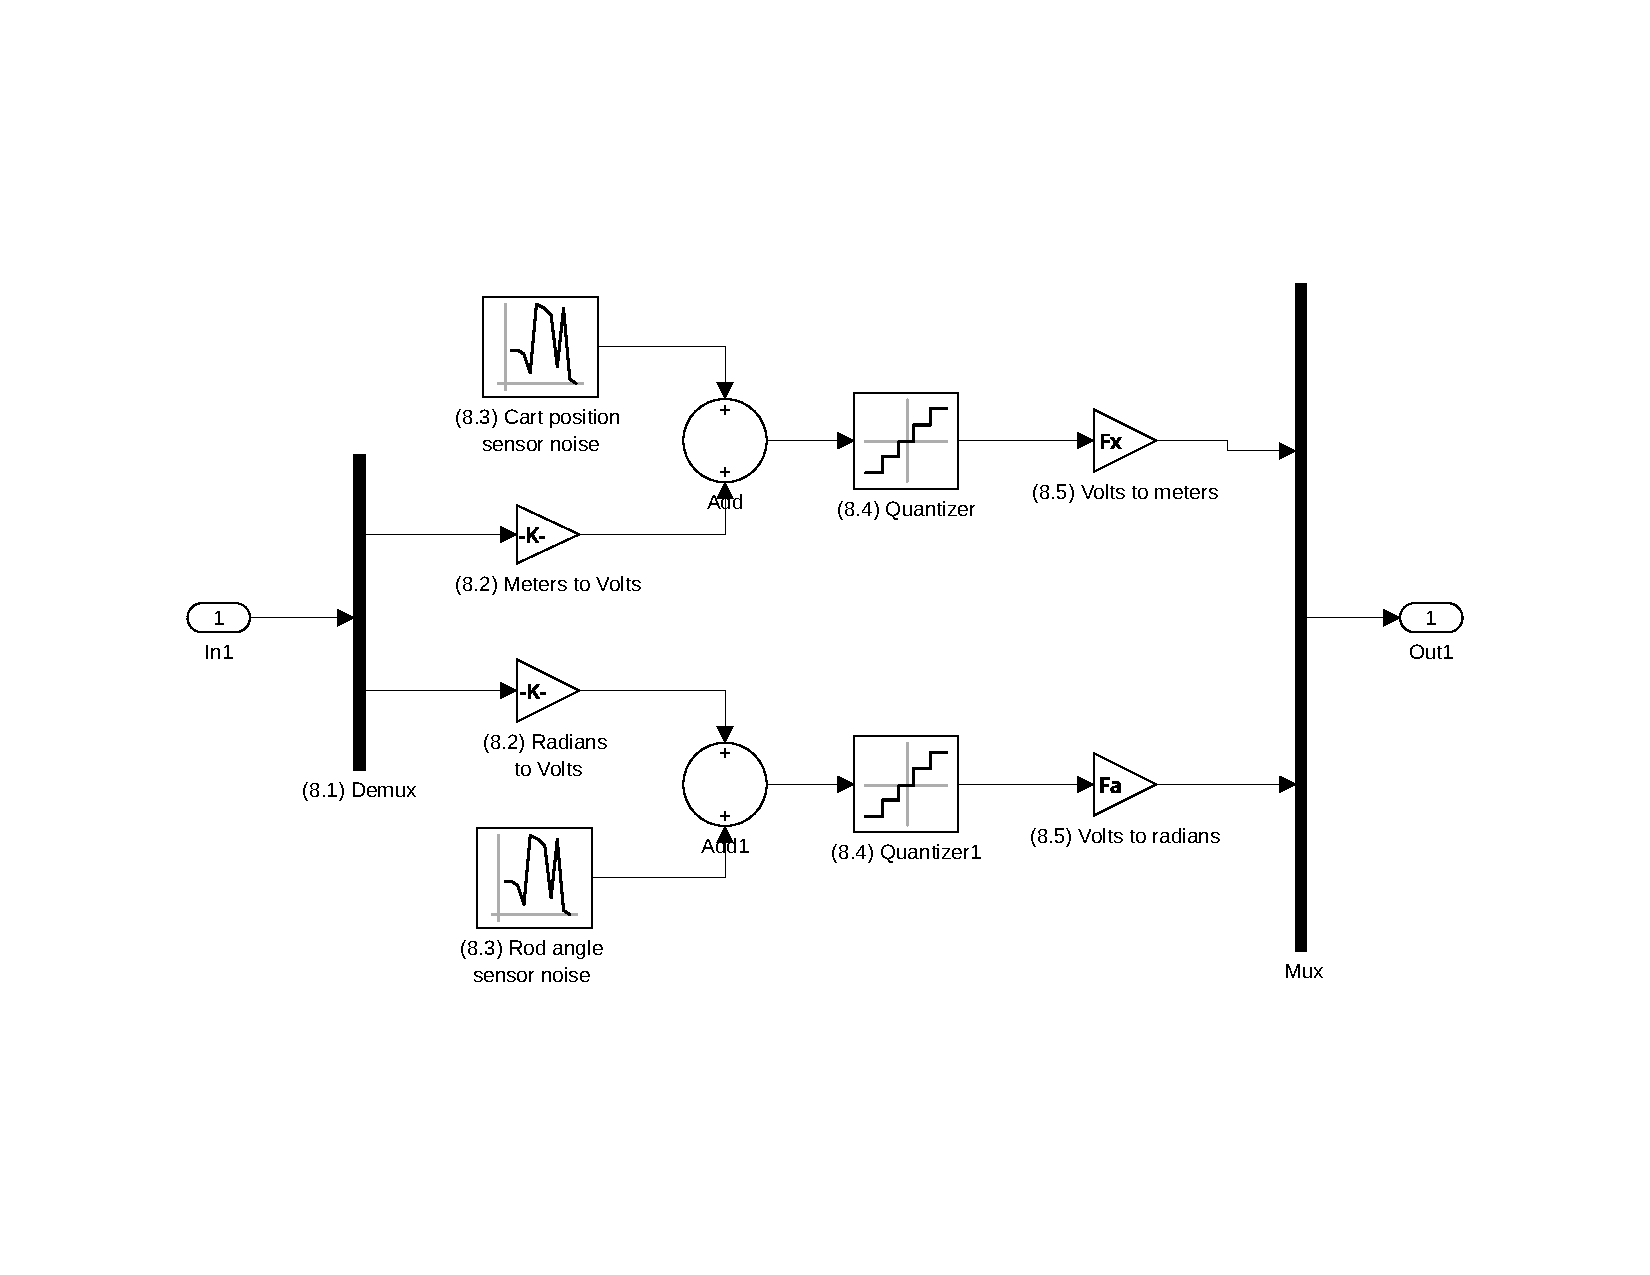
\includegraphics[width=0.8\textwidth]{figures/quantizer.pdf}
    \caption{The quantization subsystem in the more realistic closed loop simulink diagram.}
    \label{fig:quantizer}
\end{figure}

\begin{figure}[htbp]
    \centering
    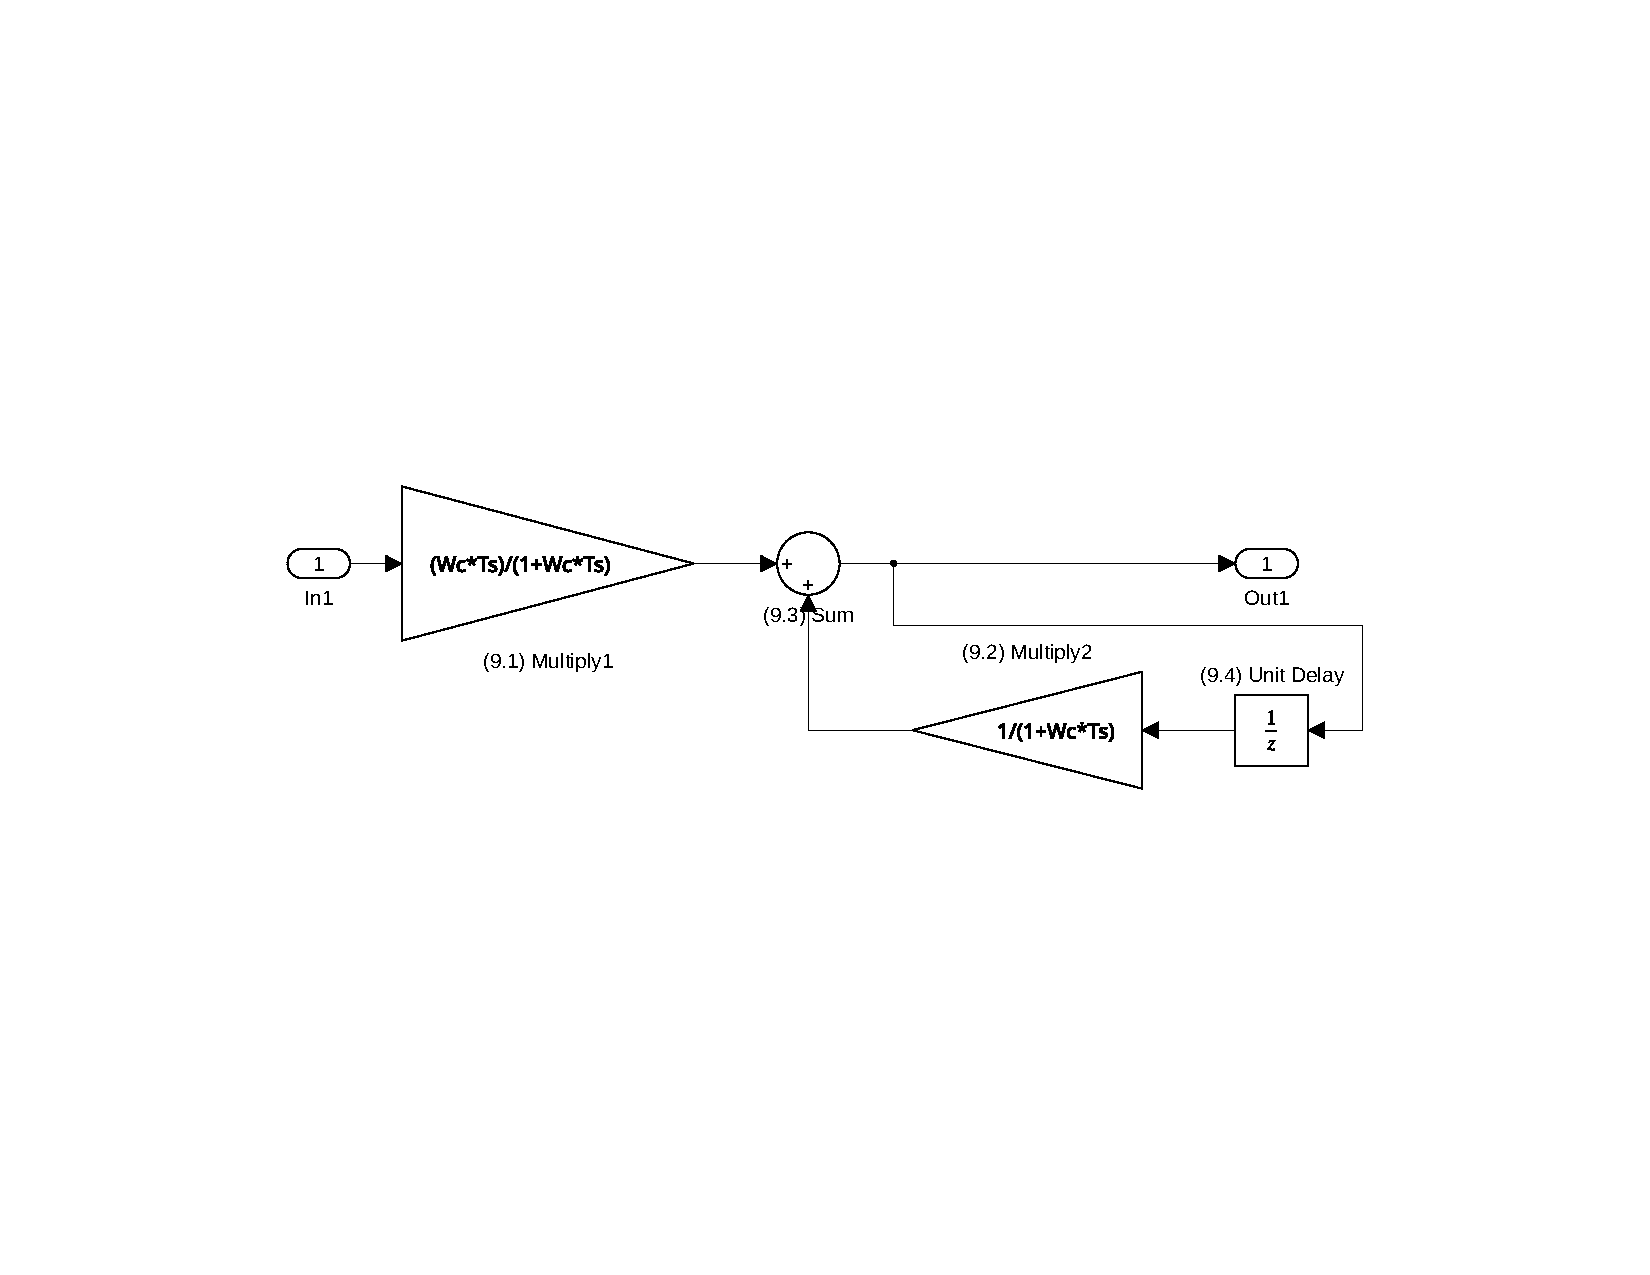
\includegraphics[width=0.8\textwidth]{figures/filter.pdf}
    \caption{The filter subsystem in the more realistic closed loop simulink diagram.}
    \label{fig:filter}
\end{figure}

\begin{figure}[htbp]
    \centering
    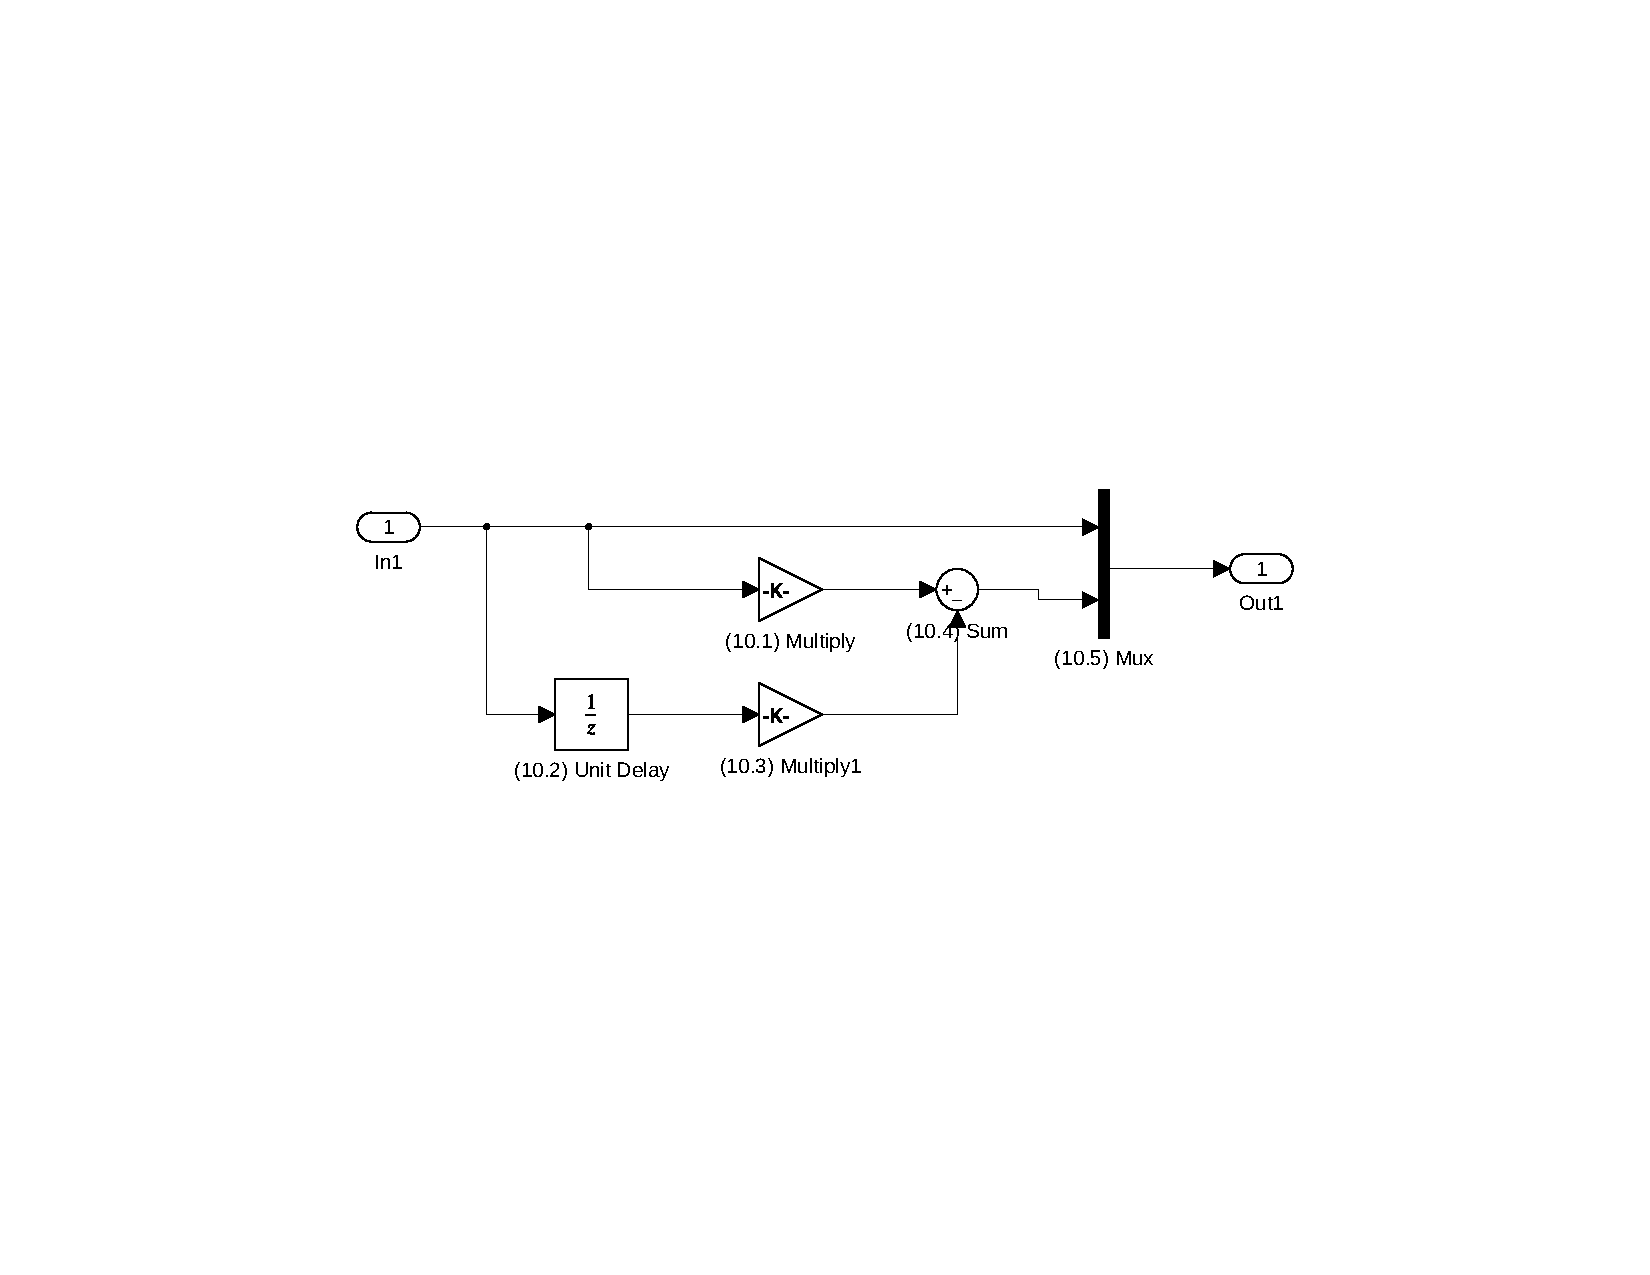
\includegraphics[width=0.8\textwidth]{figures/differentiation.pdf}
    \caption{The differentiation subsystem in the more realistic closed loop simulink diagram.}
    \label{fig:differentiation}
\end{figure}

\begin{figure}[htbp]
  \centering
  \begin{subfigure}{0.45\textwidth}
    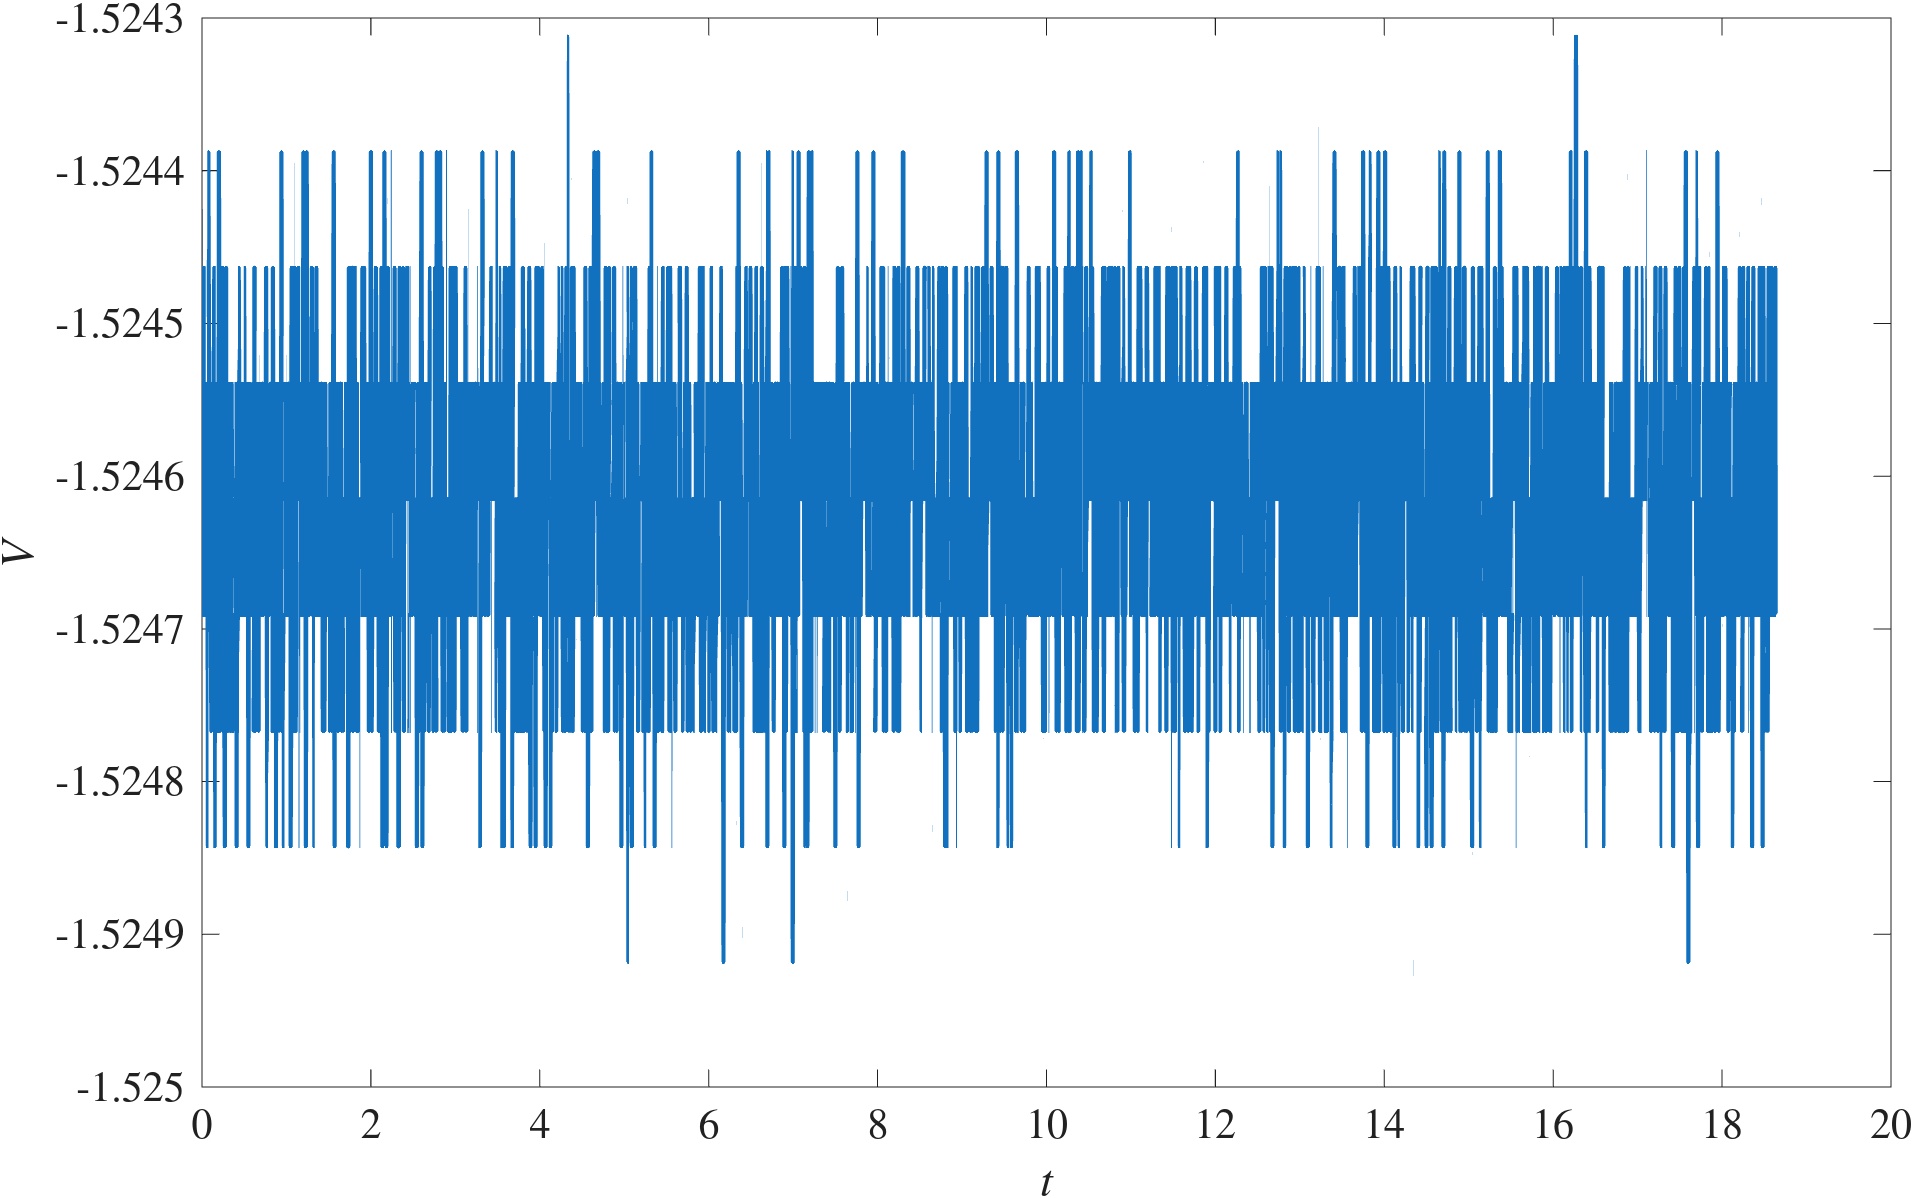
\includegraphics[width=\linewidth]{figures/angle_sensor_data.png}
    \caption{Measurements of the sensor on the rod when the rod is stationary. }
  \end{subfigure}
  \begin{subfigure}{0.45\textwidth}
    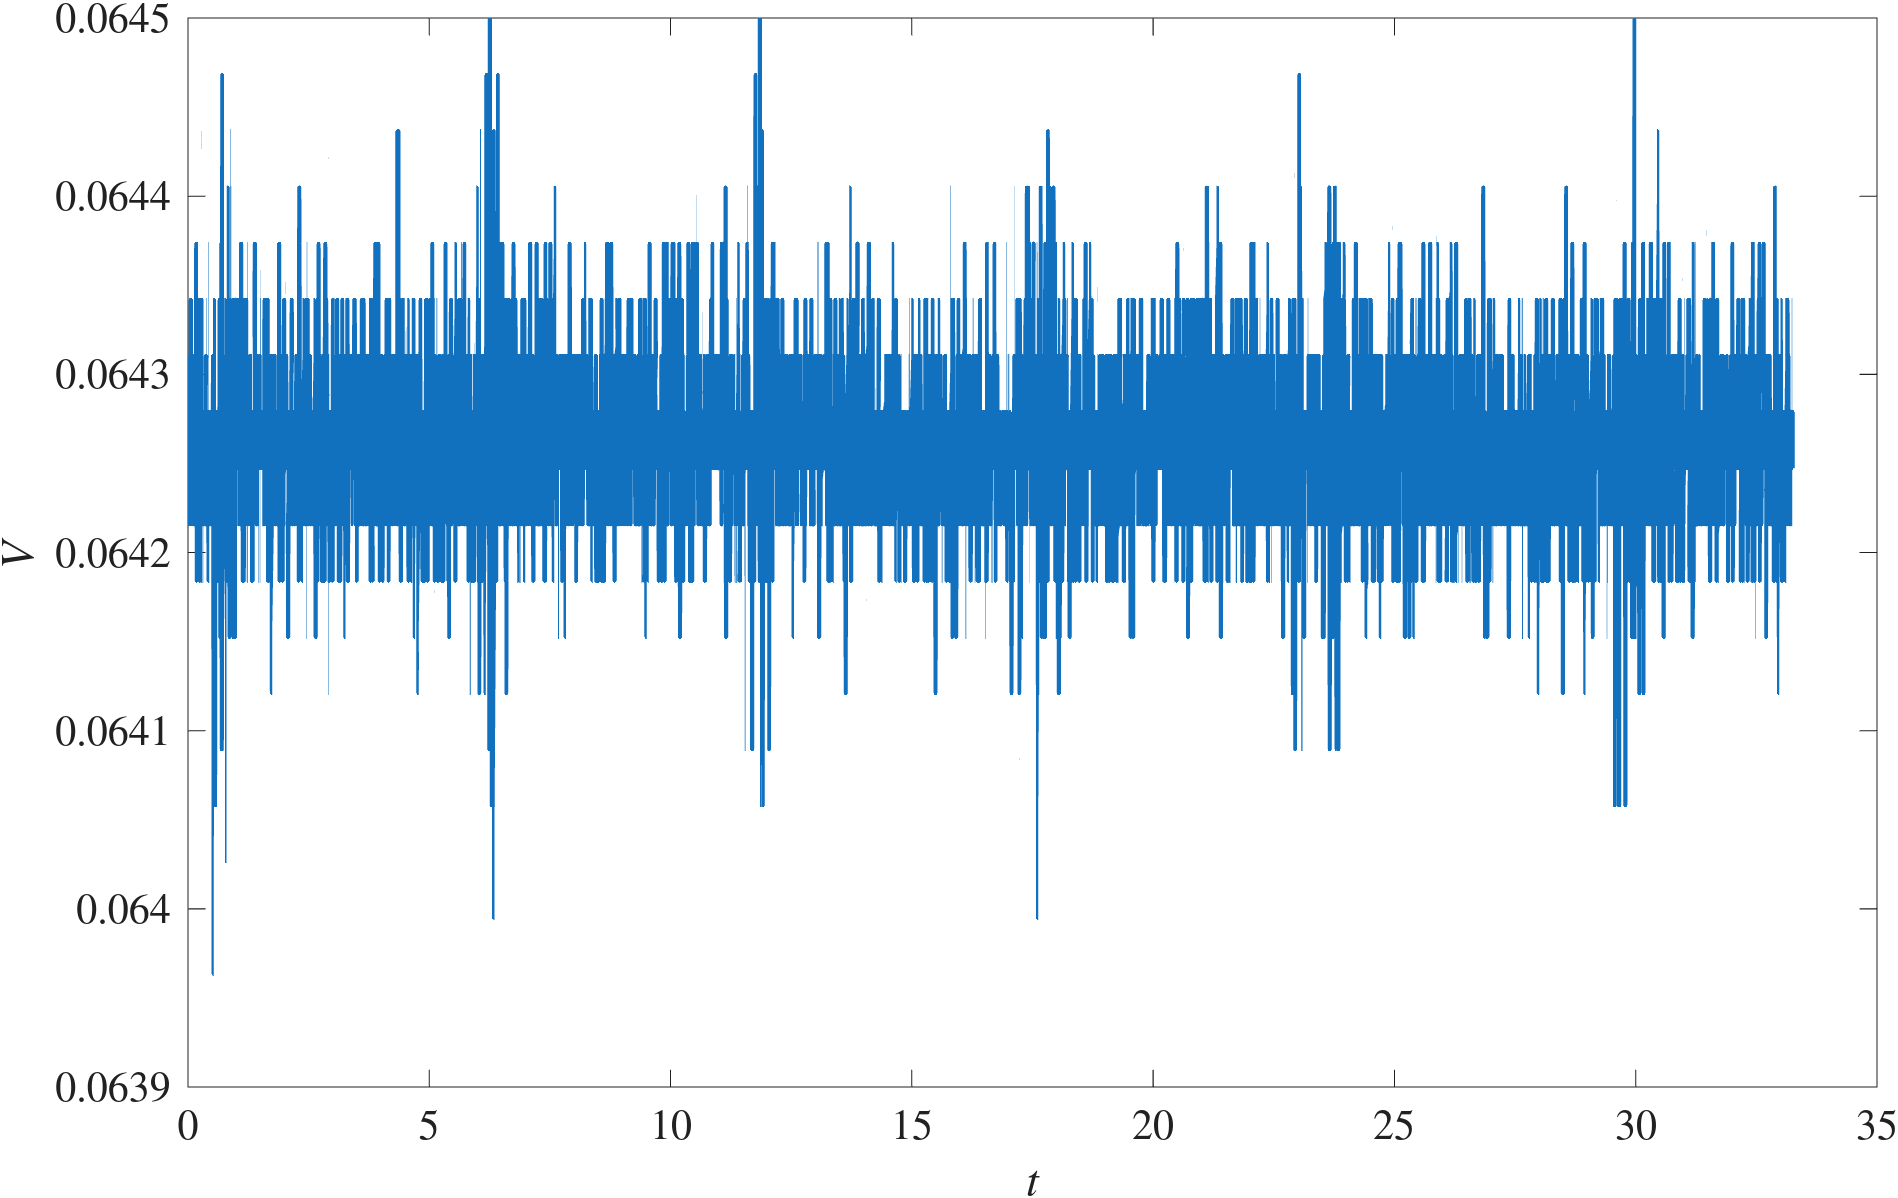
\includegraphics[width=\linewidth]{figures/position_sensor_data.png}
    \caption{Sensor Measurements of the sensor of the cart position when the rod is resting and no voltage is applied.}
  \end{subfigure}
  \caption{Plots the measurements of the sensors when the setup is in rest. The rod is layed down and no voltage is applied. This data is used to calculate the experimental variance of teh sensor noise. These calculations are used to set the random number generators in the simulink diagram of section \ref{realistic_closed_loop}.}
  \label{fig:model_selection}
\end{figure} 

\FloatBarrier
\subsection{Setpoint Change}

Figure \ref{fig:real1} plots the response of the system to a set-point change of 10 cm for the realistic closed loop system with a controller computed by LQR with $Q_1$ and $R_1$ and a cut-off frequency of 2 Hz. Compared to figure \ref{fig:step_4}, the states and the control action evolve differently. The trajectories are more oscillatory and the settling time of $x$ is longer. Most notably, the other states, $\alpha, \dot{\alpha}$ and $\dot{x}$, have increased in value. All of these observations indicate the we need increase $Q_{3,3}$ and $Q_{4,4}$. We expect that increasing $Q_{3,3}$ and $Q_{4,4}$ will repress the oscillations and reduce the peaks of the states $\alpha, \dot{\alpha}$ and $\dot{x}$. The control action will also be reduced in magnitude. The settling time of $x$ will increase as a result. 
 \begin{figure}[htbp]
  \centering
  \begin{subfigure}{0.45\textwidth}
    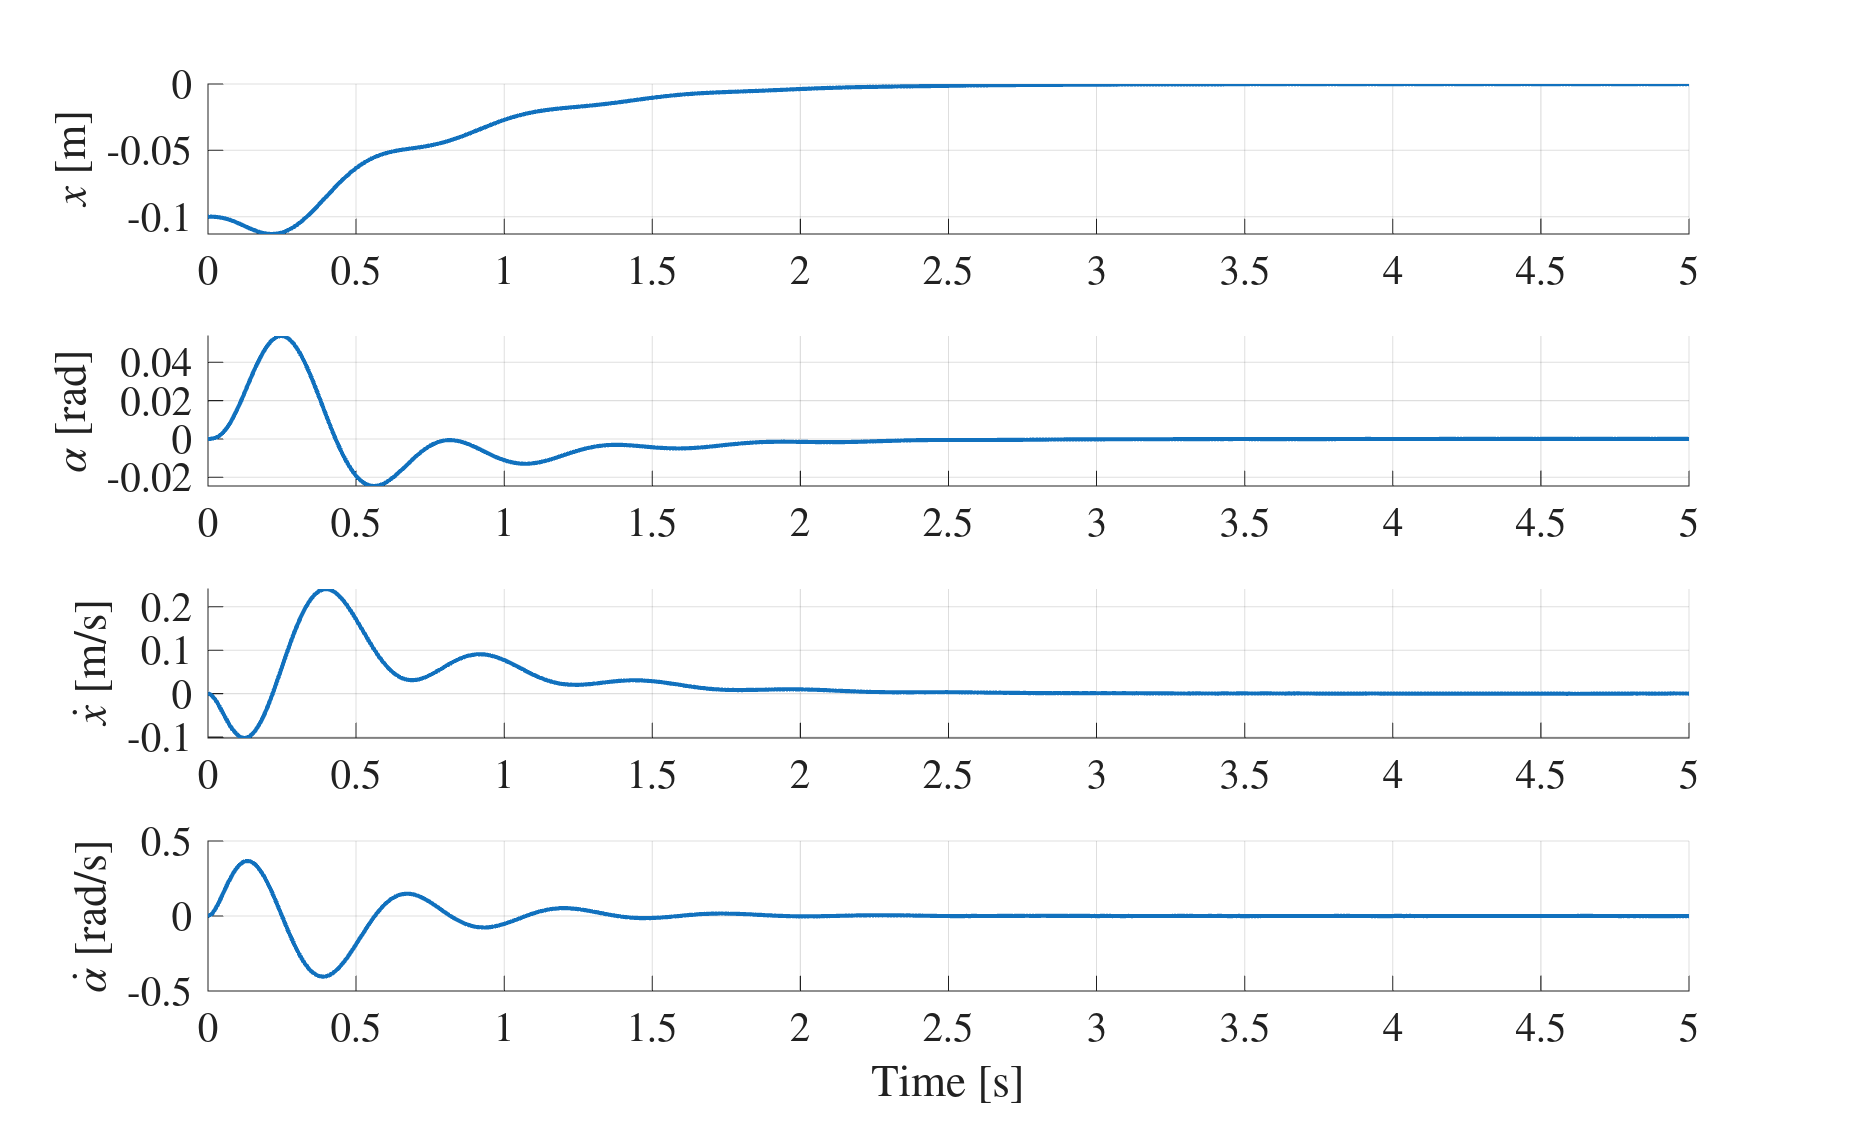
\includegraphics[width=\linewidth]{figures/real_states1.png}
    \caption{States evolution.}
  \end{subfigure}
  \begin{subfigure}{0.45\textwidth}
    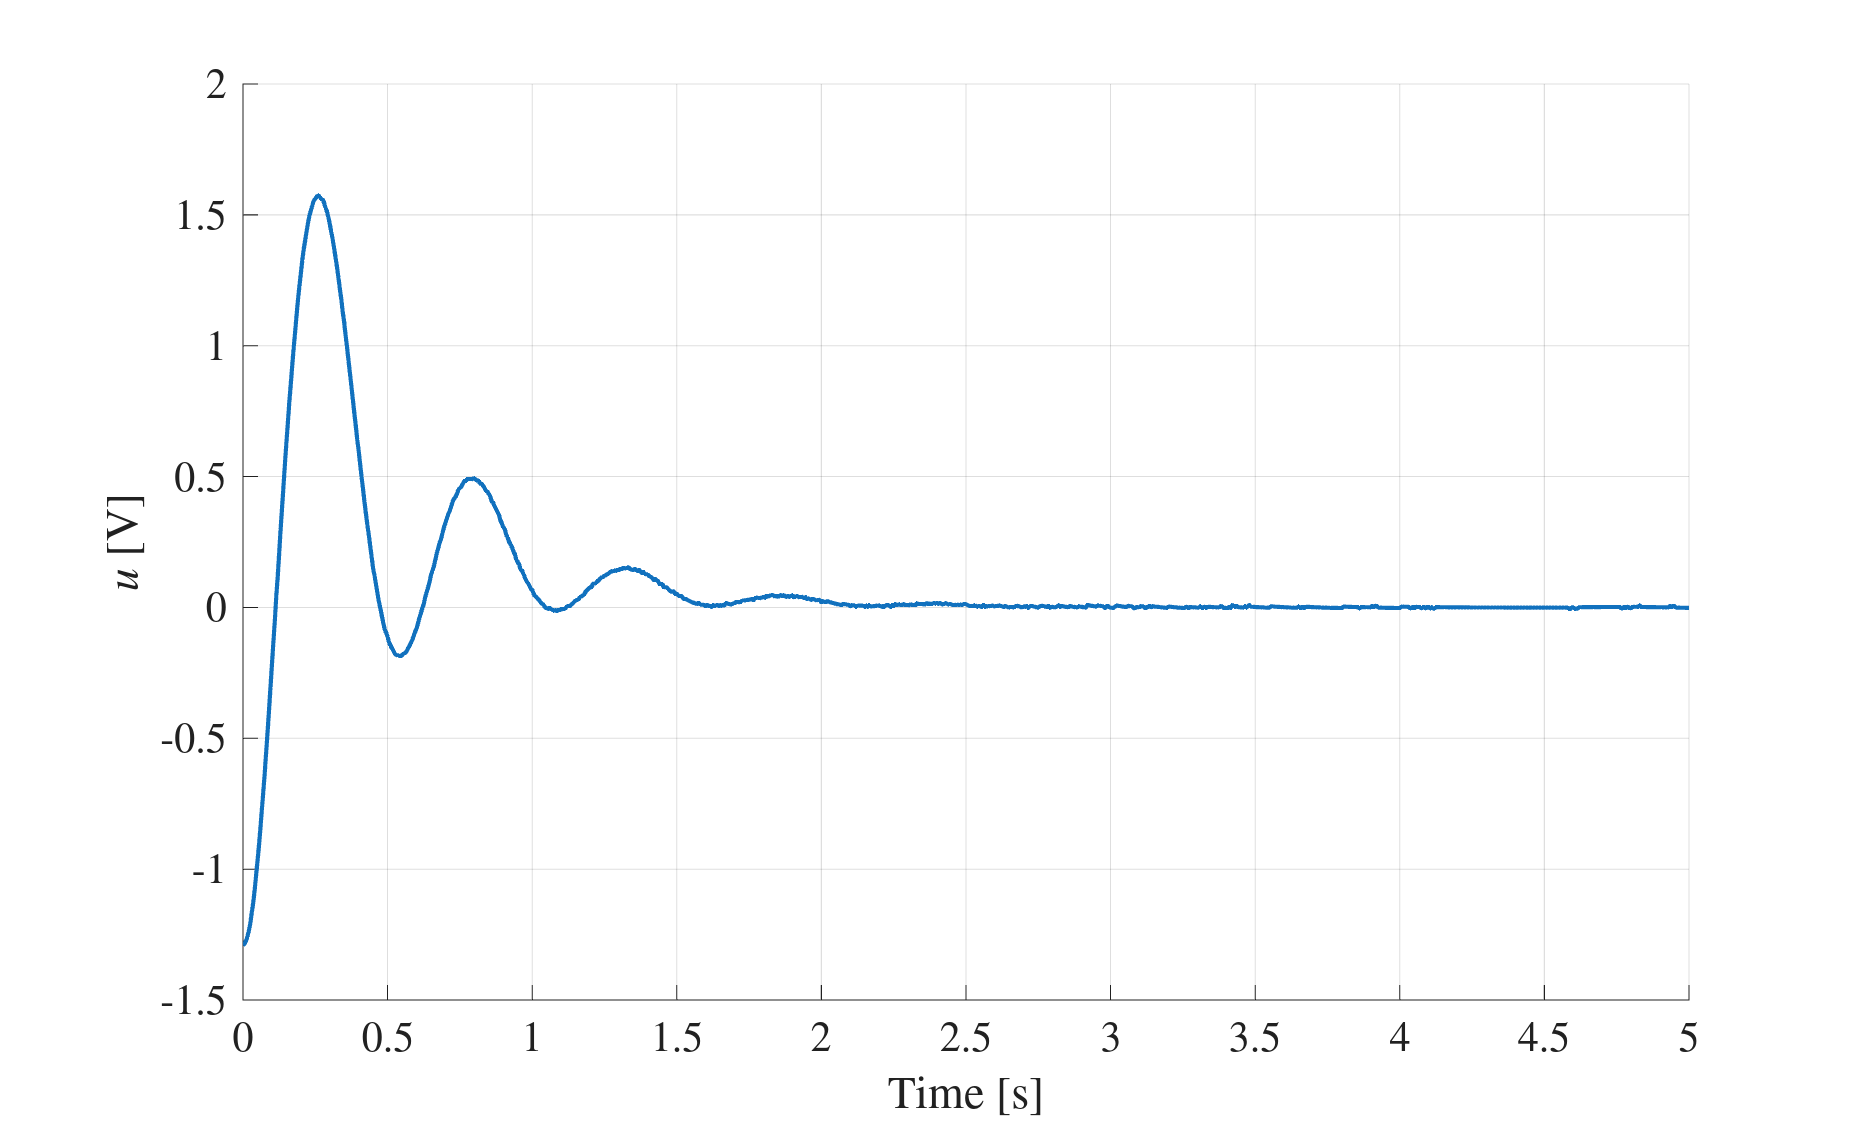
\includegraphics[width=\linewidth]{figures/real_volt1.png}
    \caption{Control action evolution.}
  \end{subfigure}
  \caption{Response of the system to a set-point change of 10 cm for the realistic closed loop system with a controller computed by LQR with $Q_1$ and $R_1$ and a cut-off frequency of 2 Hz. The settling time of $x$ is 2.6164, the maximum angle is 0.0537 radians and the maximum absolute voltage is 1.5744 Volts.}
  \label{fig:real1}
\end{figure} 

\FloatBarrier
In figure \ref{fig:real2}, we plot the evolution of the states and the control action for 

\begin{equation}
  Q_2 = 
  \begin{bmatrix}
     5.0 && 0 && 0 && 0 \\
    0 && 8.0  && 0 && 0 \\
    0 && 0 && 1.0 && 0 \\
    0 && 0 && 0 && 3.0 \\
  \end{bmatrix}, \quad
  R_2 = 0.03.
\end{equation}
Figure \ref{fig:real2} realises the expected behaviour. The states and the control action are less oscillatory and the peaks of the states $\alpha, \dot{\alpha}$ and $\dot{x}$ are reduced. The peak of the control action is also smaller in magnitude. The settling time of $x$ has increased as a result. The settling time of $x$ is now 3.8301 seconds. This could be due to the filter having a large cutoff frequency. A large cutoff frequency can remove the actual system dynamcs, making the controller more slow. If the controller is not fast enough, in the real setup, $Q_{1,1}$ will be increased. The maximum angle has decreased from 0.0537 radians to 0.0152 radians and the maximum absolute voltage has decreased from 1.5744 Volts to 1.2910 Volts. Overall, these are good improvements compared to figure \ref{fig:real1}, but the controller seems to be too slow. 

\begin{figure}[htbp]
  \centering
  \begin{subfigure}{0.45\textwidth}
    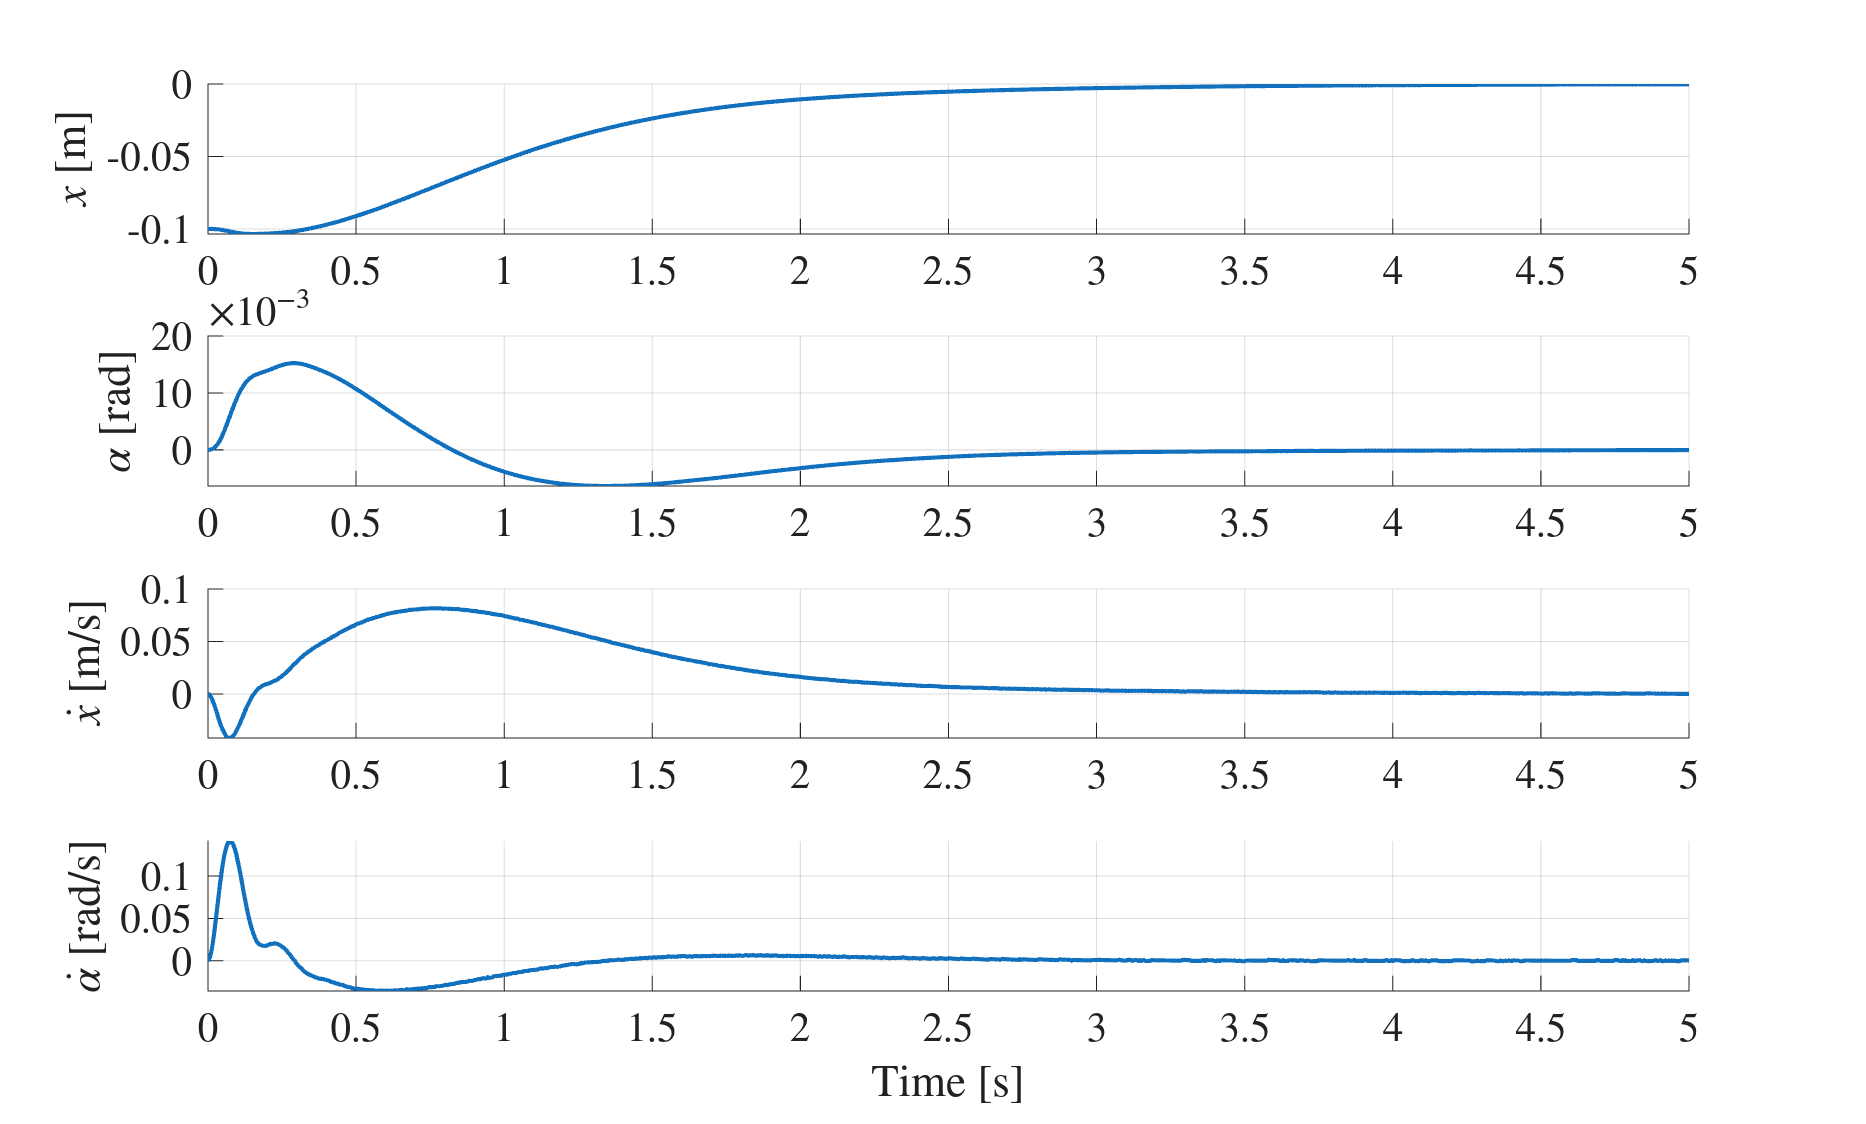
\includegraphics[width=\linewidth]{figures/real_states2.png}
    \caption{States evolution.}
  \end{subfigure}
  \begin{subfigure}{0.45\textwidth}
    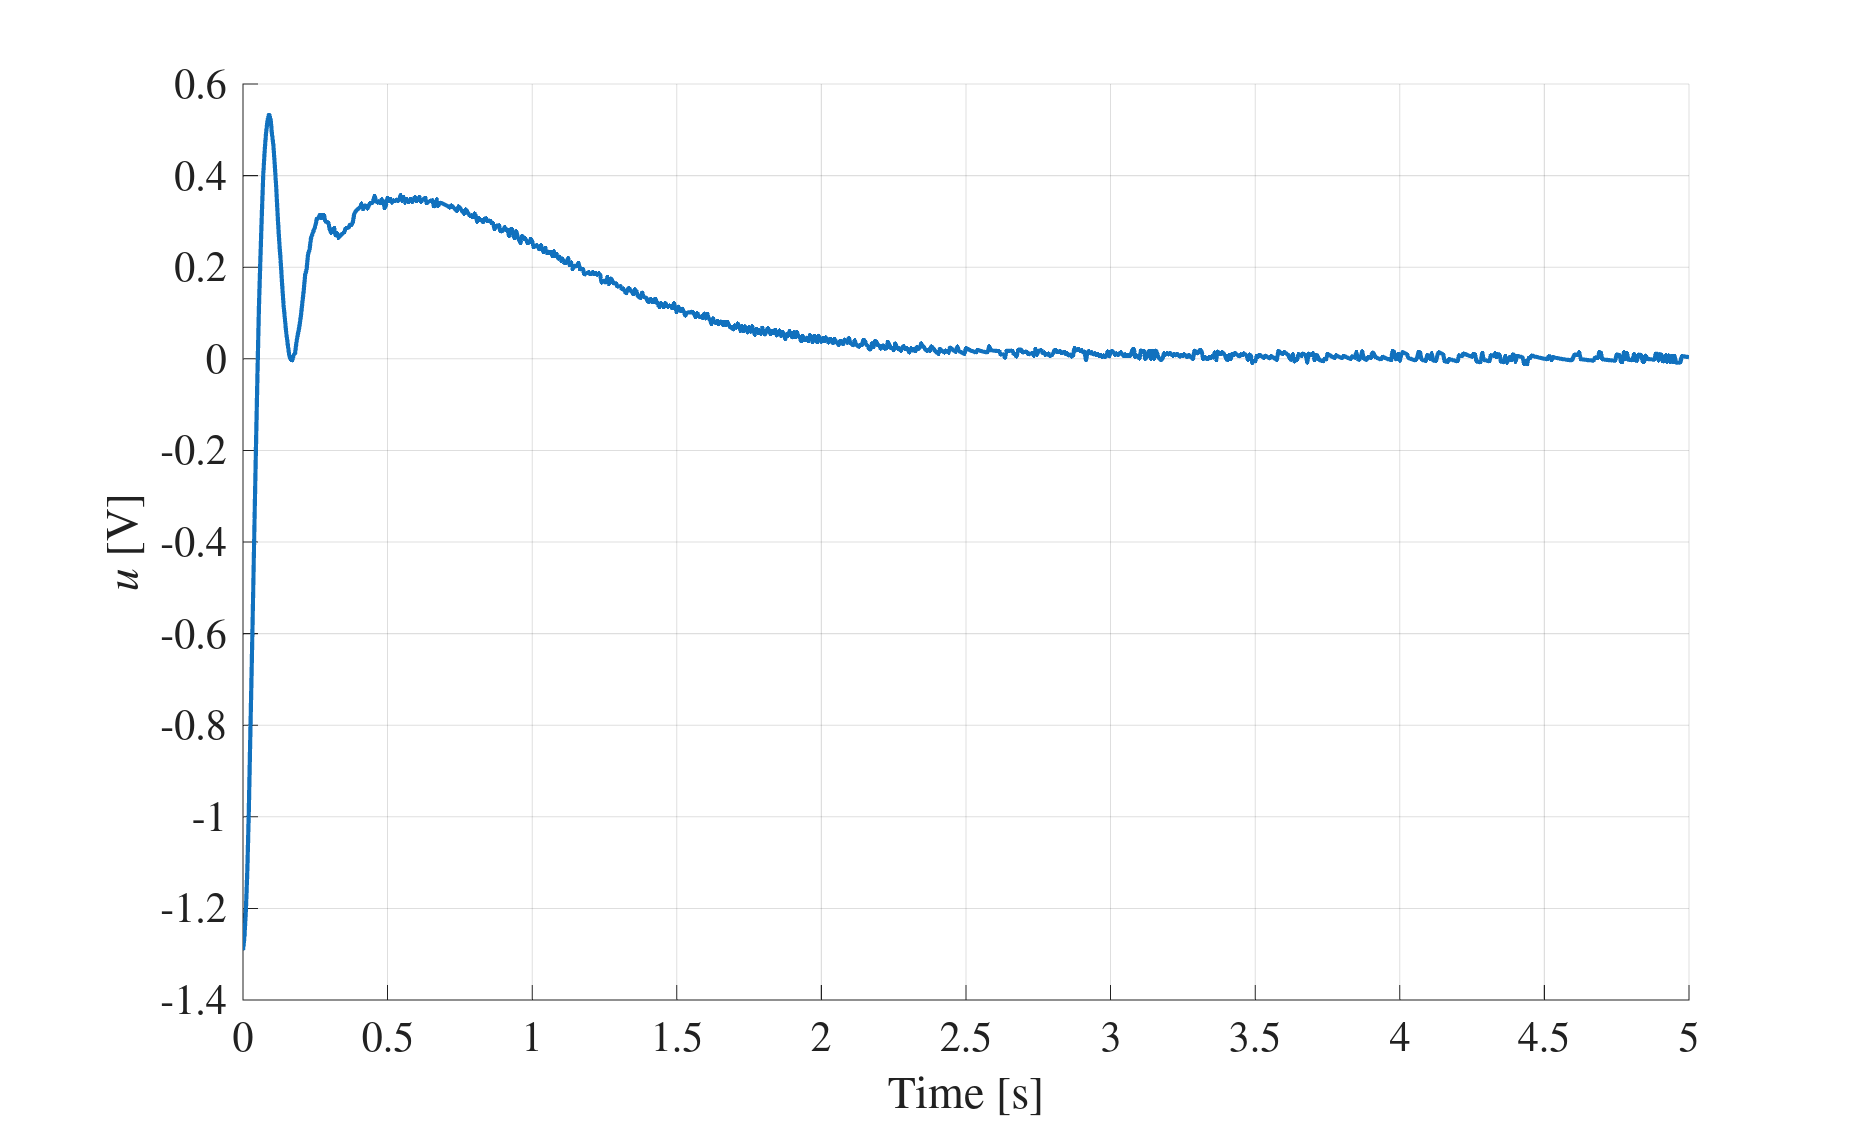
\includegraphics[width=\linewidth]{figures/real_volt2.png}
    \caption{Control action evolution.}
  \end{subfigure}
  \caption{Response of the system to a set-point change of 10 cm for the realistic closed loop system with a controller computed by LQR with $Q_2$ and $R_2$ and a cut-off frequency of 2 Hz. The 5\% threshold settling time of $x$ is 3.8301, the maximum angle is 0.0152 radians and the maximum absolute voltage is 1.2910 Volts.}
  \label{fig:real2}
\end{figure} 


\subsection{Influence of the Cut-Off Frequency}

The filter is placed directly after the sensor measurements. Its role is to remove the noise that orginated from the sensors and smooth out the outgoing signal. If the outgoing signal is not smooth enough, then the finite difference calculation of the states $\dot{x}$ and $\dot{\alpha}$ will be also affected. However, if the cut-off frequency is too low, then the filter will remove the actual system dynamics and the controller will be slow to react. Thus, our goal is to find the ideal cut-off frequency that removes the noise and smooths out $\dot{x}$ and $\dot{\alpha}$, but does not remove the actual system dynamics. \\
\\
We investigate the influence of the cut-off frequency on the behaviour of the system through multiple simulations and comparing them to each other. We would like to confirm the previous intuition and find an optimal cut-off frequency. Figure \ref{fig:real_freq_01}, \ref{fig:real_freq} and \ref{fig:real_freq_50} plot the evolution of the states and the control action of a set-point change of 10 cm for the realistic closed loop system with a controller computed by LQR with $Q_2$ and $R_2$ and cut-off frequencies, $f \in \{0.1, 0.3, 0.5, 1.0, 2.0, 5.0, 10.0, 50.0\}$ Hz. \\
\\
From figure \ref{fig:real_freq}, we notice that for lower frequencies the system behaves with higher frequency and larger amplitude. Compare for $f = 0.3$ Hz to $f = 10$ Hz and notice the states $\alpha, \dot{\alpha}, \dot{x}$ and the control action. For $f = 10.0$ Hz, the system oscillates with a lower frequency and a smaller amplitude. For $f = 0.3$ Hz, the system oscillates with a high frequency and a large amplitude. Basically, the system reacts sluggish for higher cut-off frequencies and reacts more quickly. Physically, when the cart tracks the set-point, it will speed up then slow down and then speed up again. It is as if the cart is being operated by a drunk driver. This analogy is very fitting, since the filter is removing important dynamics of the system, it can be seen as an impaired receptor to the controller. From this point of view, we can also explain the many peaks (high frequency) and large amplitude. Only when the dynamics of the system are large enough will the controller be able to act upon it. However, once these dynamics are large, the controller will send a large control action to compensate for its delayed response. This in turn will momentarily stabilize the system, where again the controller will have to wait until the dynamics are sufficiently large enough to act upon. This explanation is supported by the evolution of the states in figure \ref{fig:real_freq}. For $f = 0.3$ the blue curve on the figure, we can see how the peaks and dips of $\alpha$ align in time with the peaks and dips of the control action. And the evolution $\alpha$ and $\dot{\alpha}$ is out of phase with $\dot{x}$.\\
\\
This behaviour is taken to its extreme in figure \ref{fig:real_freq_01} for $f = 0.1$ Hz. Once the system detects the velocity of $\alpha$, it is already too late. The controller will compensate with a control action that is too large for the actuator. The actuator will then saturate and the system will be unstable. \\
\\
However, when the cut-off frequency is too high, we also observe high frequency oscillations, but with smaller amplitude. This is observed in figure \ref{fig:real_freq_50} for $f = 50$ Hz. As the cut-off frequency is too big, sensor noise is not adequately filtered and reaches the controller. The noise affects finite-difference calculations non-smooth trajectories. This is clearly visible by the trajectory of $\dot{x}$ and $\dot{\alpha}$. This in turn affects the controller performance. The system is overly responsive\\



\begin{figure}[htbp]
  \centering
  \begin{subfigure}{0.45\textwidth}
    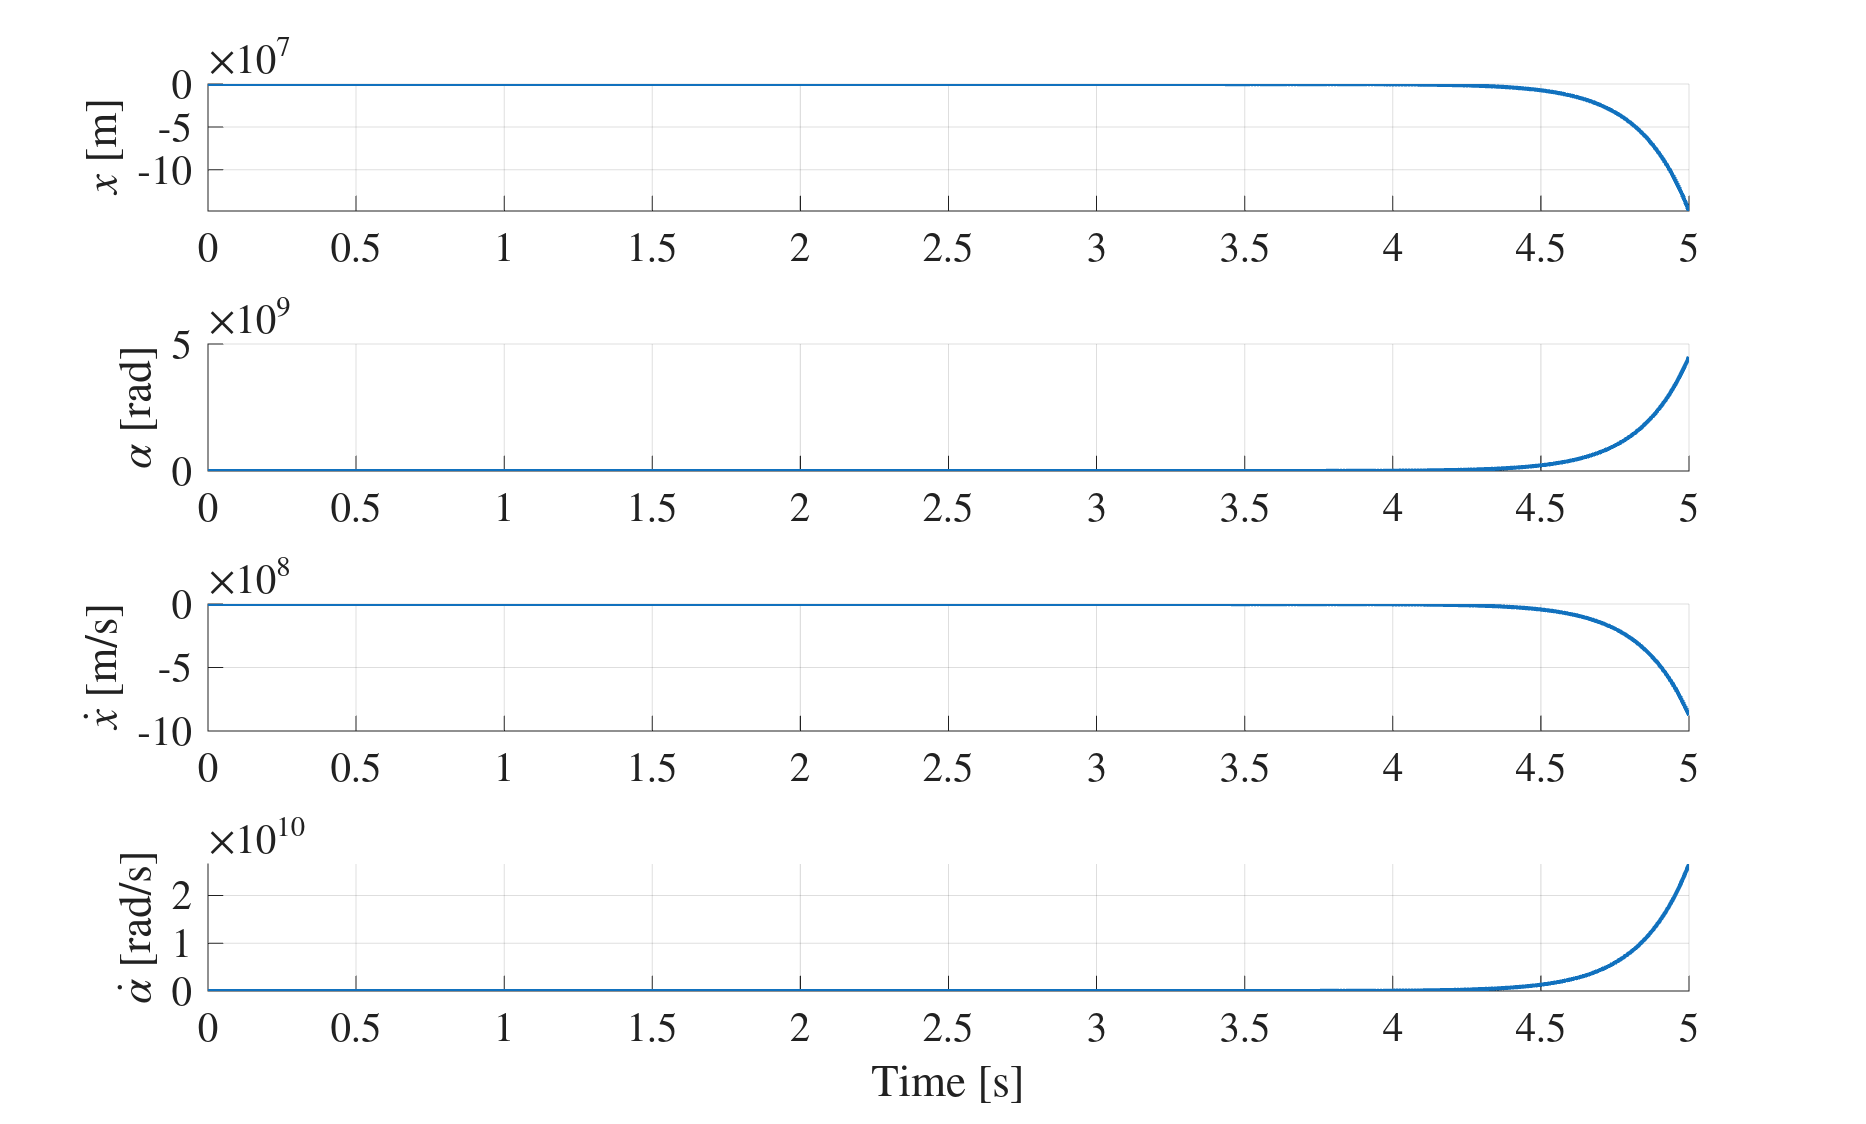
\includegraphics[width=\linewidth]{figures/real_freq_states_01.png}
    \caption{States evolution.}
  \end{subfigure}
  \begin{subfigure}{0.45\textwidth}
    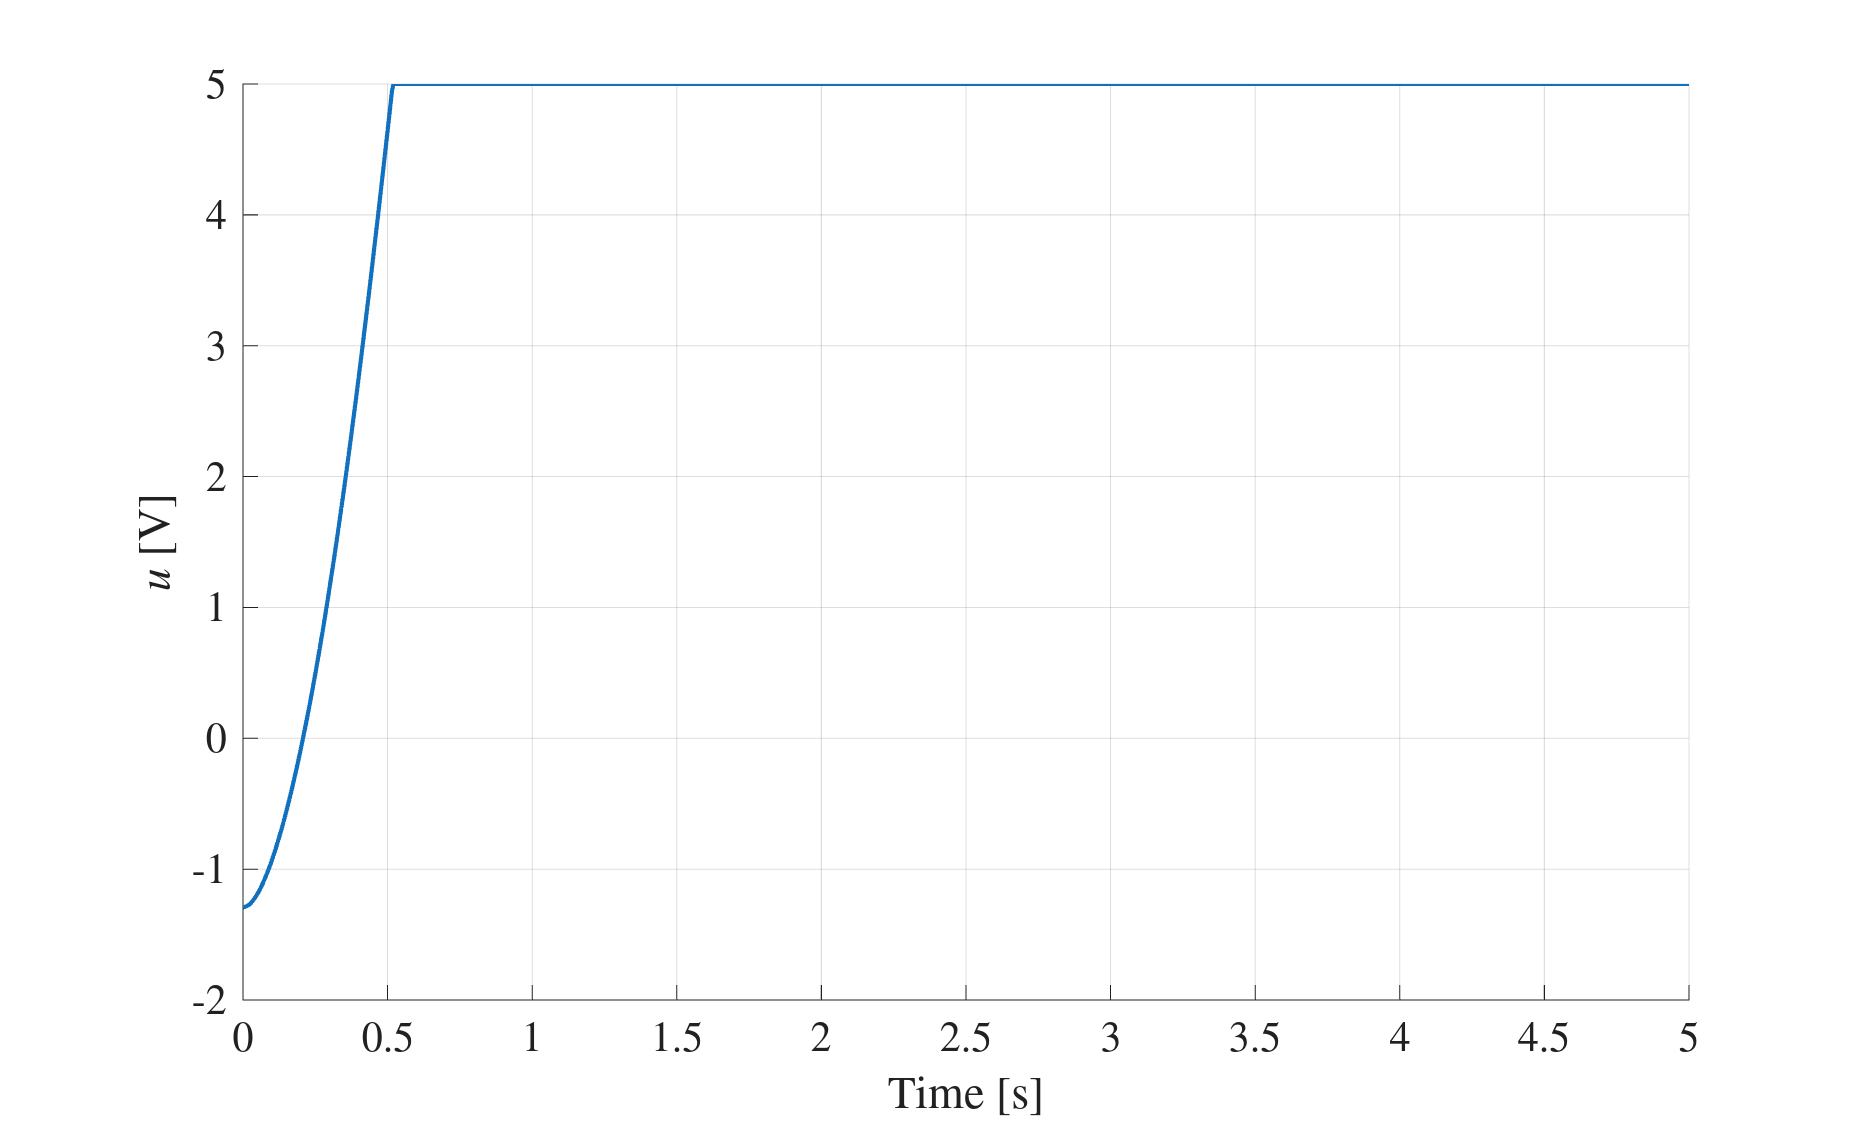
\includegraphics[width=\linewidth]{figures/real_freq_volt_01.png}
    \caption{Control action evolution.}
  \end{subfigure}
  \caption{Response of the system to a set-point change of 10 cm for the realistic closed loop system with a controller computed by LQR with $Q_2$ and $R_2$ and a cut-off frequency of 0.1 Hz.}
  \label{fig:real_freq_01}
\end{figure} 

\begin{figure}[htbp]
  \centering
  \begin{subfigure}{0.45\textwidth}
    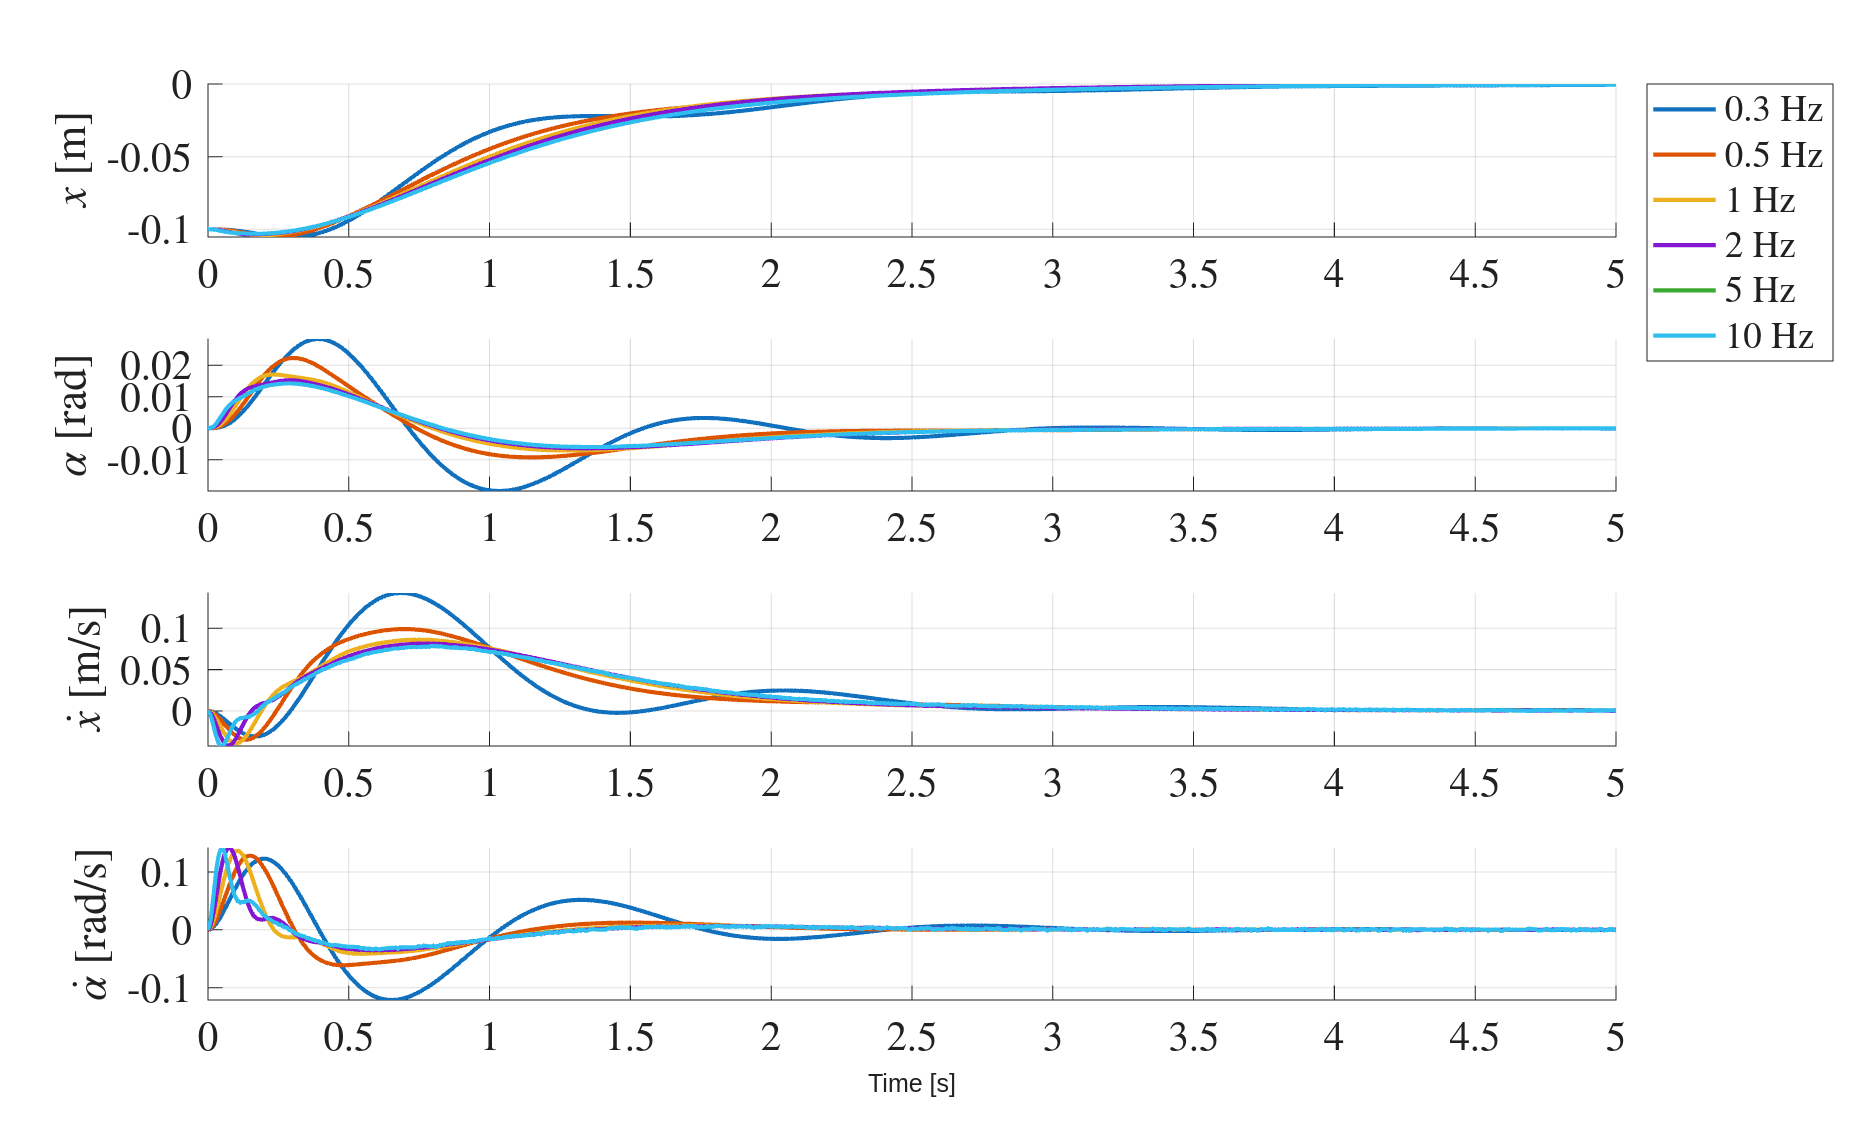
\includegraphics[width=\linewidth]{figures/real_freq_states.png}
    \caption{States evolution.}
  \end{subfigure}
  \begin{subfigure}{0.45\textwidth}
    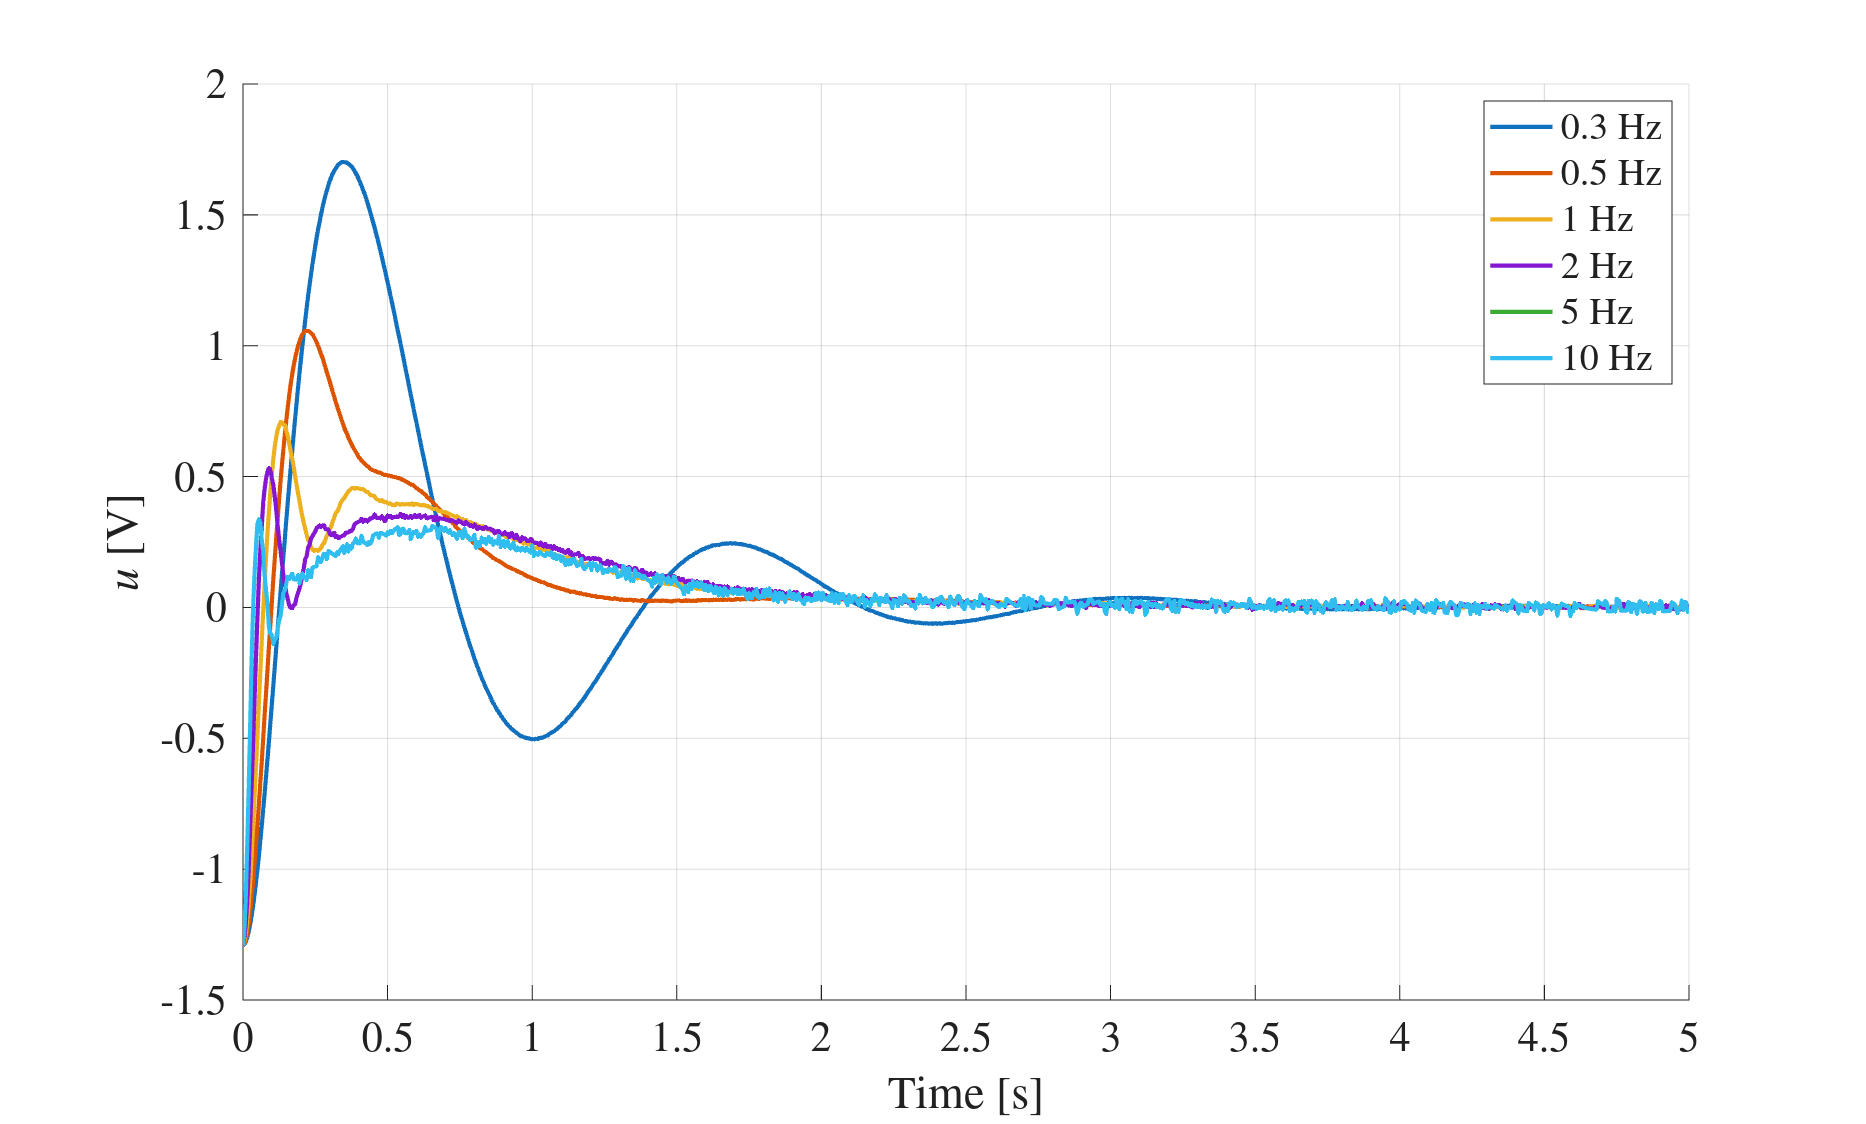
\includegraphics[width=\linewidth]{figures/real_freq_volt.png}
    \caption{Control action evolution.}
  \end{subfigure}
  \caption{Response of the system to a set-point change of 10 cm for the realistic closed loop system with a controller computed by LQR with $Q_2$ and $R_2$ and cut-off frequencies, $f \in \{0.3, 0.5, 1.0, 2.0, 5.0, 10.0\}$.}
  \label{fig:real_freq}
\end{figure} 

\begin{figure}[htbp]
  \centering
  \begin{subfigure}{0.45\textwidth}
    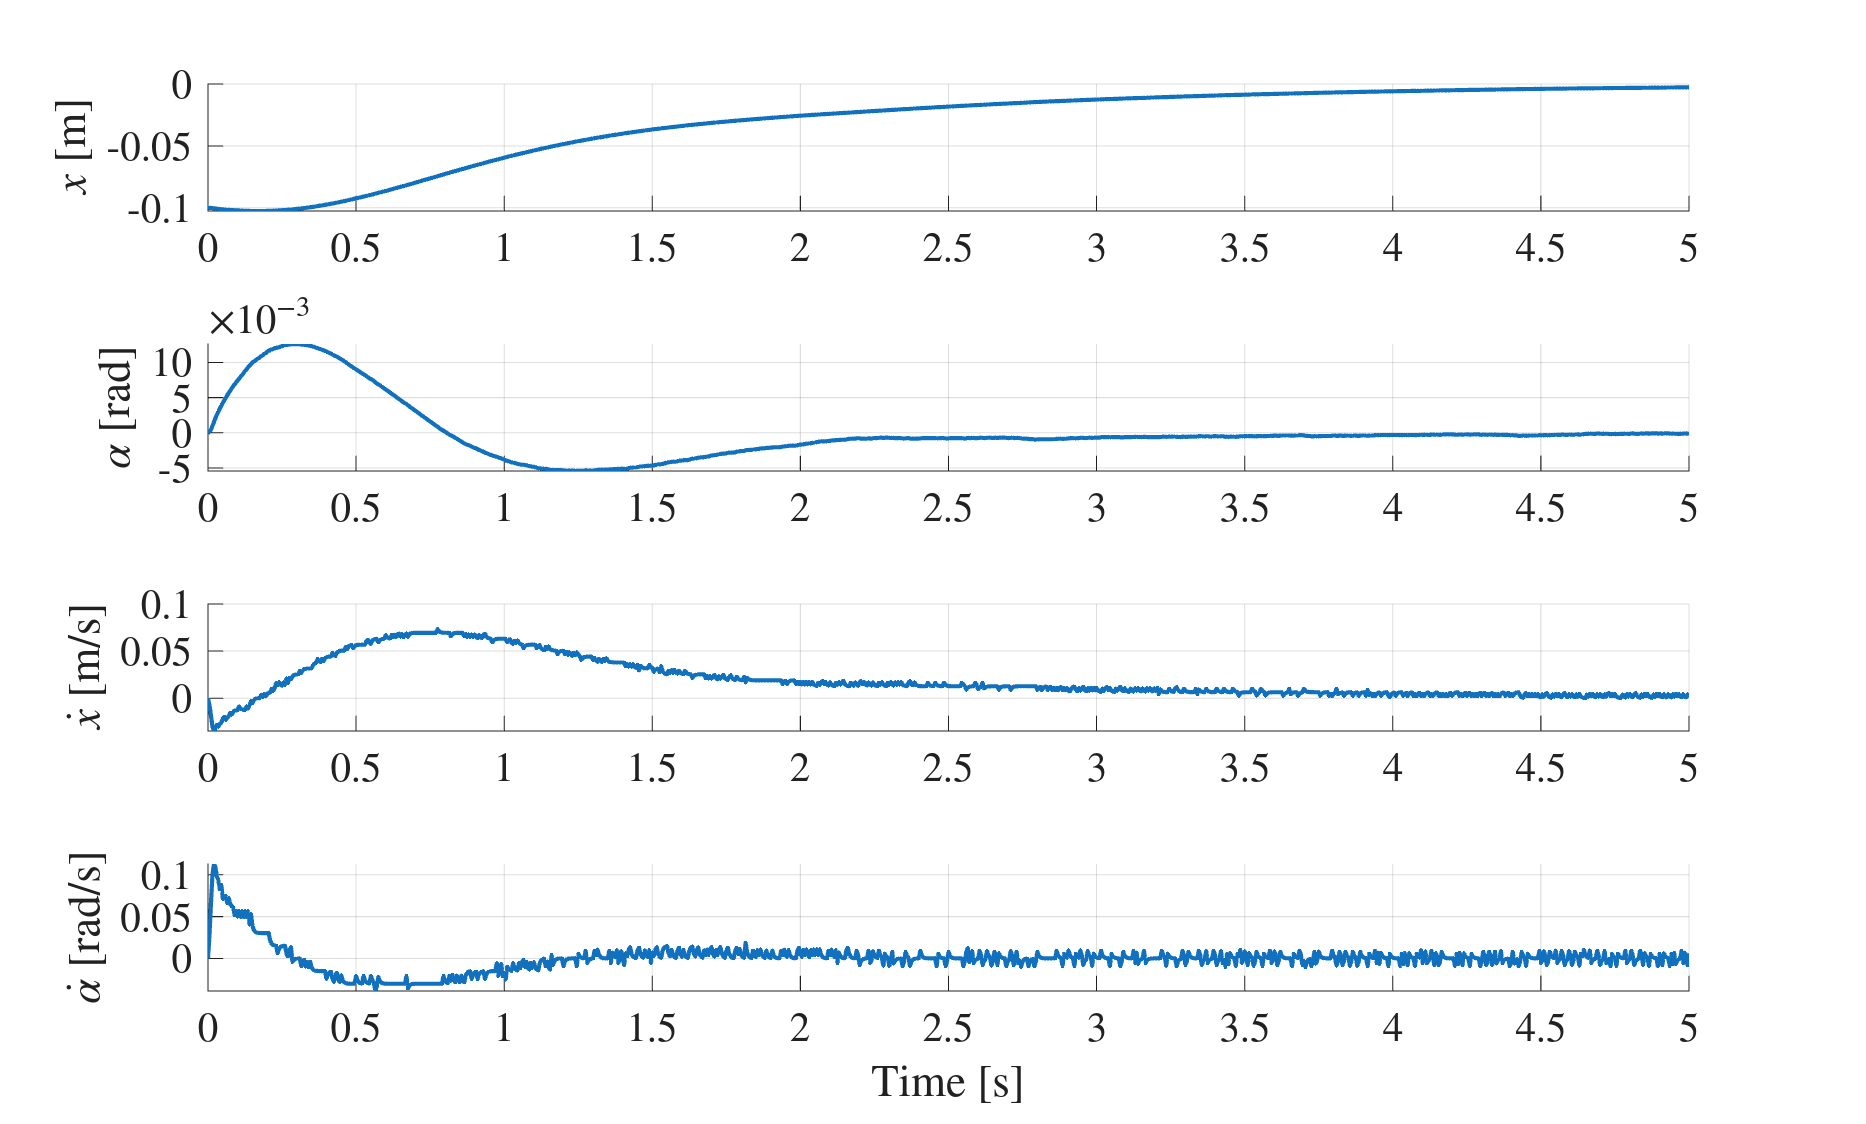
\includegraphics[width=\linewidth]{figures/real_freq_states_50.png}
    \caption{States evolution.}
  \end{subfigure}
  \begin{subfigure}{0.45\textwidth}
    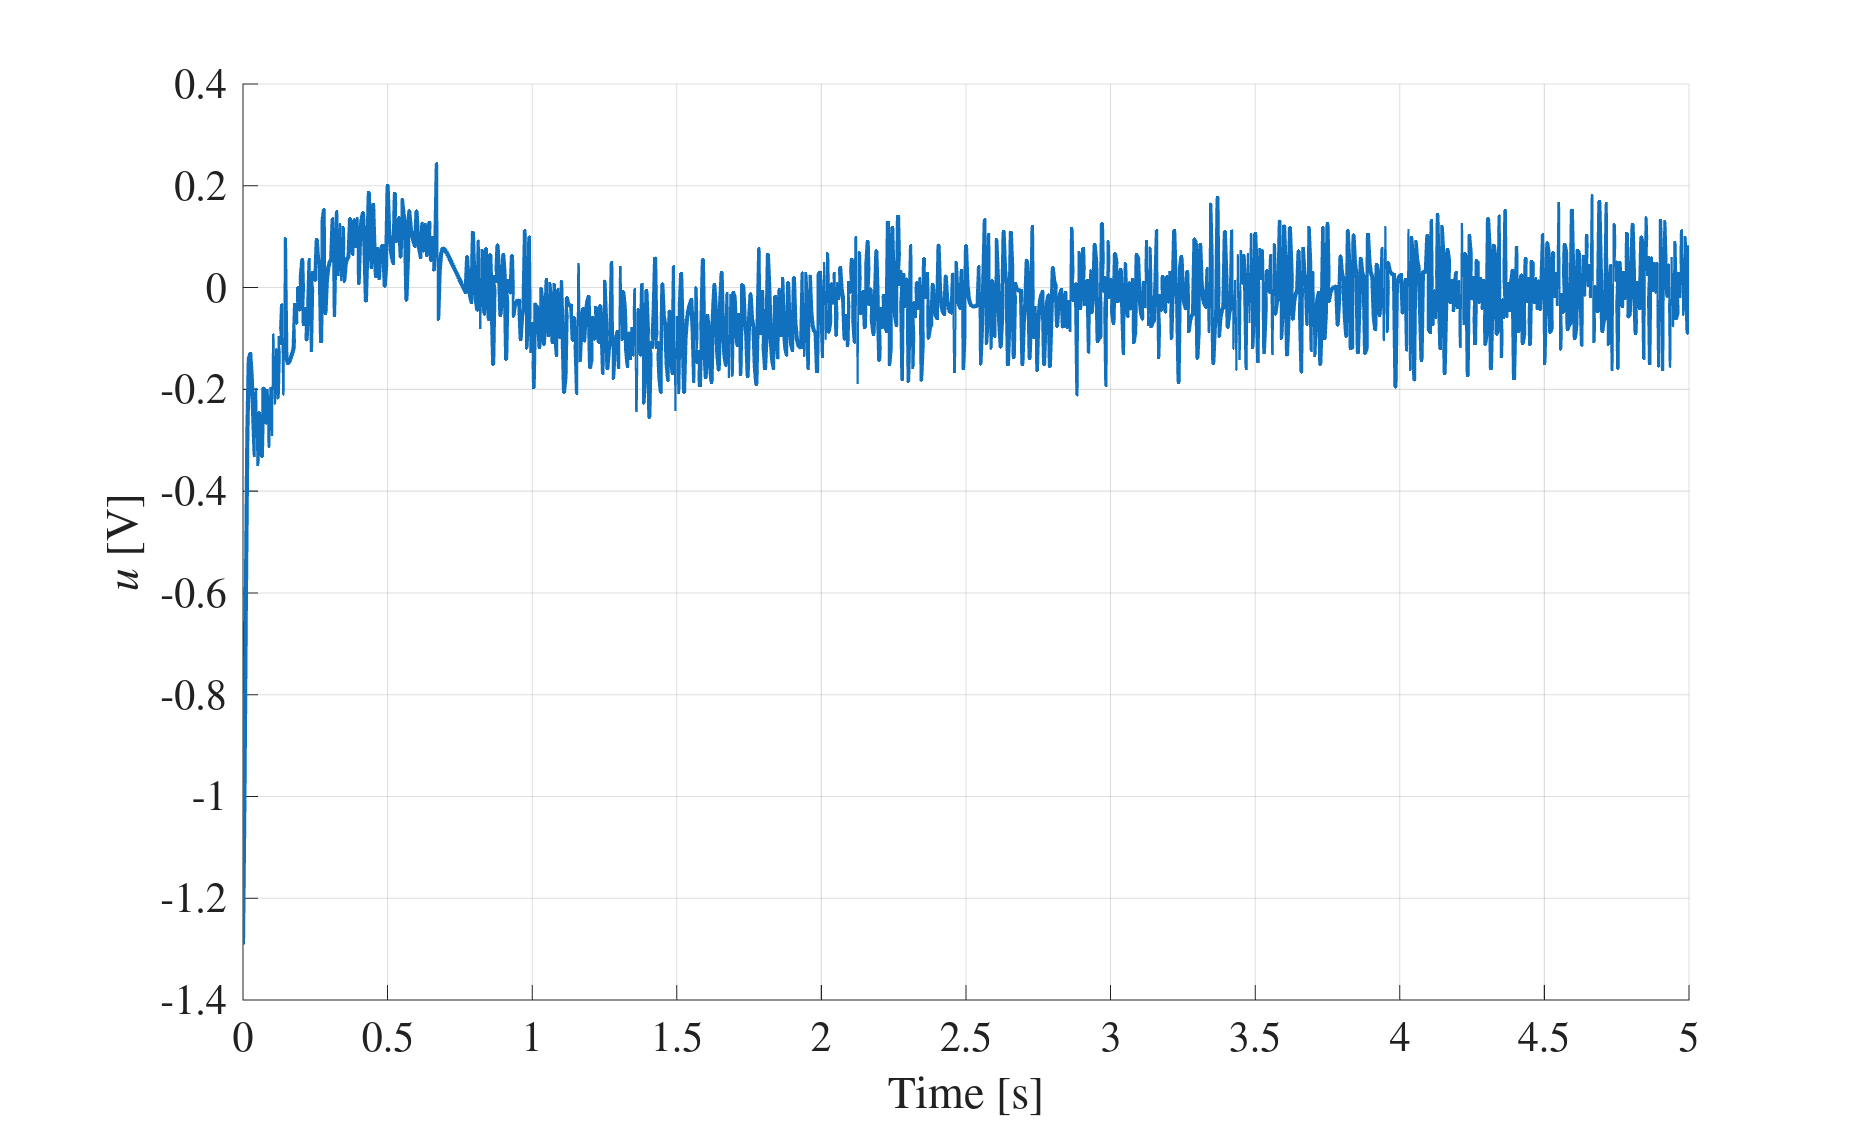
\includegraphics[width=\linewidth]{figures/real_freq_volt_50.png}
    \caption{Control action evolution.}
  \end{subfigure}
  \caption{Response of the system to a set-point change of 10 cm for the realistic closed loop system with a controller computed by LQR with $Q_2$ and $R_2$ and a cut-off frequency of 50 Hz.}
  \label{fig:real_freq_50}
\end{figure} 

\FloatBarrier

\section{Proof of the Pudding} \label{labo}

\subsection{Simulink Diagram}

Figure \ref{fig:template} provides the simulink diagram that is used to control the setup in real time. The filter, differentiation, set-point, and control action blocks are the same as in section \ref{realistic_closed_loop}. The Analog output block sends the control action to the DC motor connected to the cart. The analag input block outputs the measurements of the sensors on the setup and computes the conversion from volts to the measurement units. In comparison to the diagram in section \ref{realistic_closed_loop}, two blocks are not present: The state-space block and the A/D converter block. The reason is that the previous diagrams were meant for simulation. The quantization already happens in the sensors and the steady-state block is the linear representation of the inverted pendulum system. The diagram in figure \ref{fig:template} is closed by the actual nonlinear system evolving in front of our eyes. And it is quantified and digitalized through the sensors present on the setup. Consequently, the diagram is a closed loop and the controller performs an LQR negative state-feedback control law.

\begin{figure}[htbp]
    \centering
    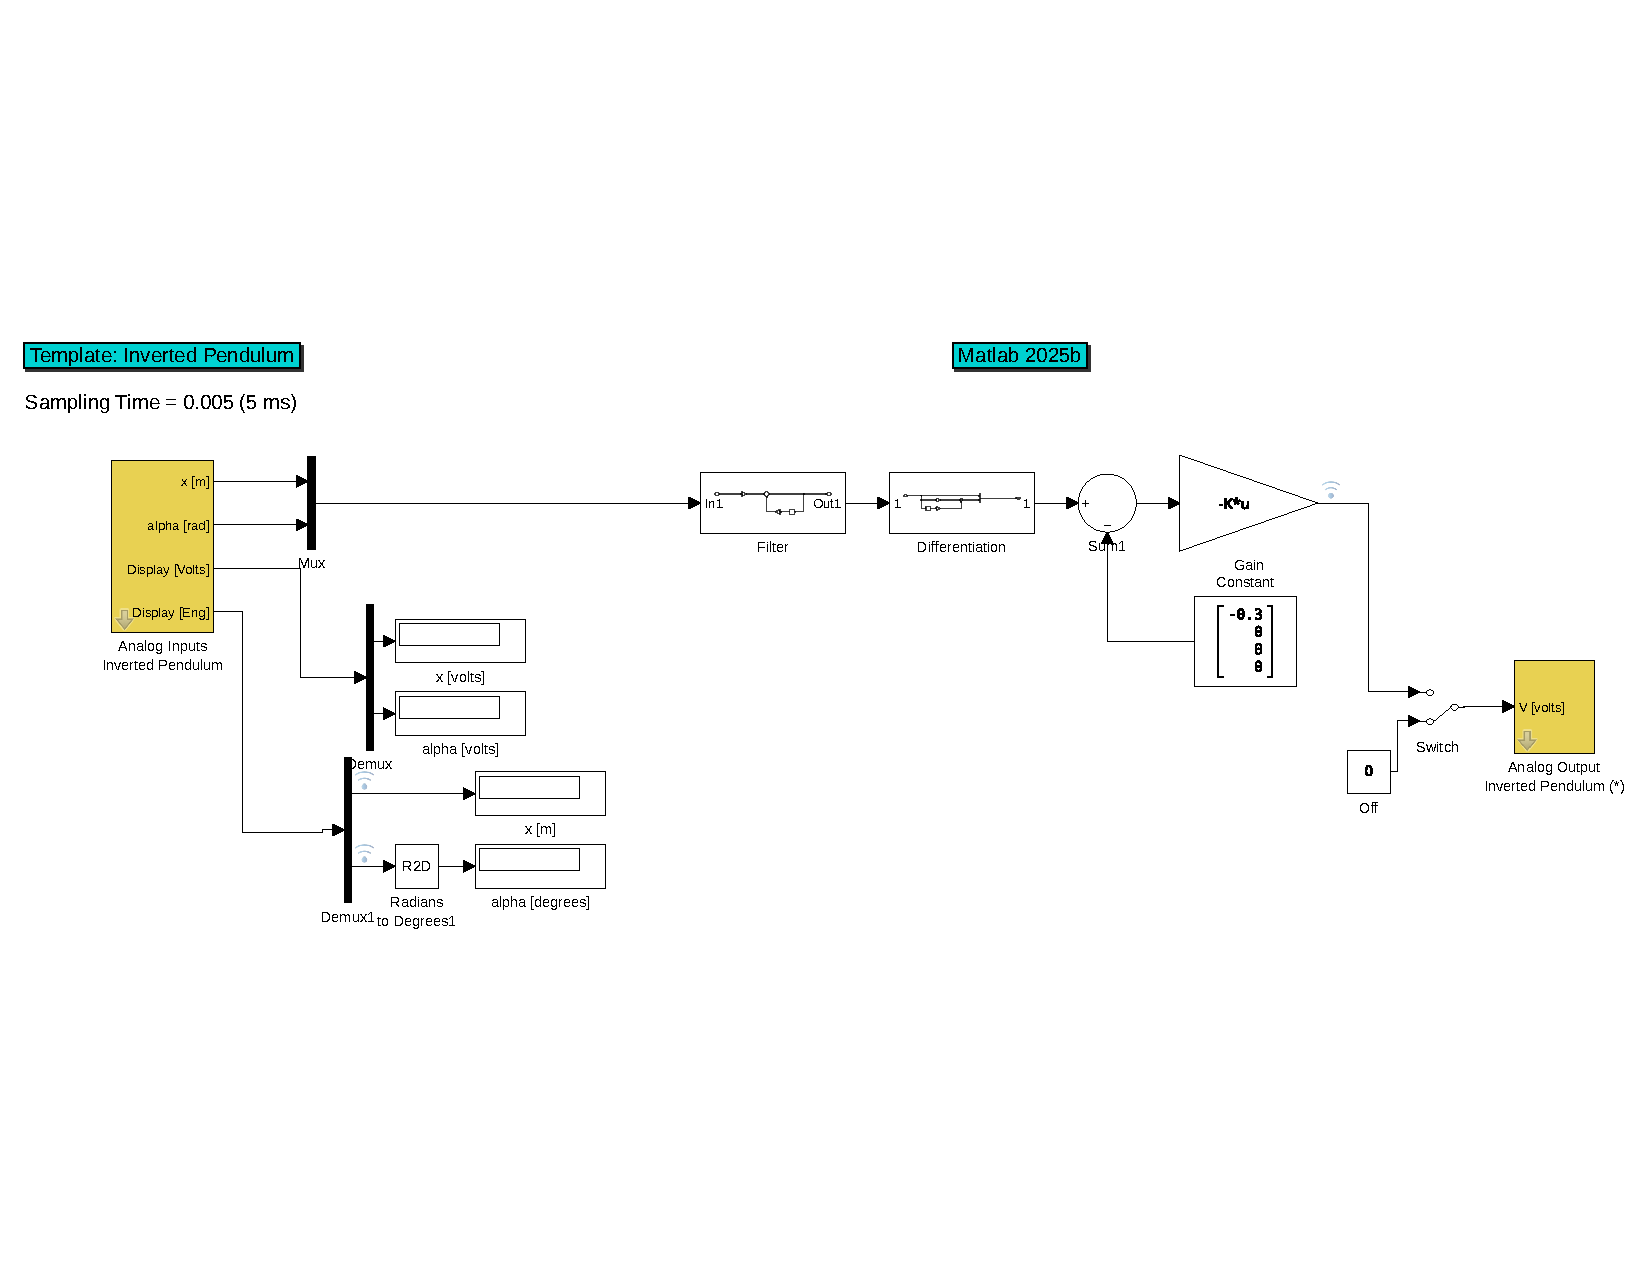
\includegraphics[width=0.8\textwidth]{figures/template_inverted_pendulum_2025b.pdf}
    \caption{Simulink diagram used in the real setup.}
    \label{fig:template}
\end{figure}

\subsection{Setpoint Tracking}





\subsection{Disturbance Rejection}
\subsection{Cut-Off Frequency}

\section{Conclusion}

lol
\end{document}









chat
Add comment         
\begin{figure}[htbp]
    \centering
    \includegraphics[width=0.7\textwidth]{figures/impulse_iir.png}
    \caption{Impulse response of the original IIR system}
    \label{fig:iir}
\end{figure}

\begin{figure}[htbp]
  \centering
  \begin{subfigure}{0.45\textwidth}
    \includegraphics[width=\linewidth]{figures/aic_exp1.png}
  \end{subfigure}
  \begin{subfigure}{0.45\textwidth}
    \includegraphics[width=\linewidth]{figures/aic_exp2.png}
  \end{subfigure}
  \caption{The normalized cost functions for estimation data, validation data and AIC-criterion
for $\sigma_{\hat{y}}$ = 0.5 (left) and $\sigma_{\hat{y}}$ = 0.05 (right). The data are generated by an IIR system with
additional output noise. The identified models are FIR models of increasing order.}
  \label{fig:model_selection}
\end{figure} 

\begin{table}[htbp]
\centering
    \begin{tabular}{lc}
        \toprule
            & \textbf{Type for $(0,0)$} \\
        \midrule
          $V < -\frac{2}{A_1}19$   &  Stable Node \\
          $-\frac{2}{A_1}19 < V < \frac{2}{A_1}$ & Stable spiral \\
          $V = \frac{2}{A_1}$ & Center \\
          $\frac{2}{A1} < V < \frac{2}{A_1}21$ & Unstable spiral \\
          $\frac{2}{A_1}21 < V$ & Unstable node \\
        \bottomrule
    \end{tabular}
    \caption{Linear classification of the equilibrium point $(0,0)$.}
    \label{tab:lin_class}
\end{table}